\documentclass[a4paper,14pt,oneside,openany]{memoir}

%%% Задаем поля, отступы и межстрочный интервал %%%

\usepackage[left=30mm, right=15mm, top=20mm, bottom=20mm]{geometry} % Пакет geometry с аргументами для определения полей
\pagestyle{plain} % Убираем стандарные для данного класса верхние колонтитулы с заголовком текущей главы, оставляем только номер страницы снизу по центру
\parindent=1.25cm % Абзацный отступ 1.25 см, приблизительно равно пяти знакам, как по ГОСТ
\usepackage{indentfirst} % Добавляем отступ к первому абзацу
%\linespread{1.3} % Межстрочный интервал (наиболее близко к вордовскому полуторному) - тут вместо этого используется команда OnehalfSpacing*

%%% Задаем языковые параметры и шрифт %%%

\usepackage[english, russian]{babel}                % Настройки для русского языка как основного в тексте
\babelfont{rm}{Times New Roman}                     % TMR в качестве базового roman-щрифта

%%% Задаем стиль заголовков и подзаголовков в тексте %%%

\setsecnumdepth{subsection} % Номера разделов считать до третьего уровня включительно, т.е. нумеруются только главы, секции, подсекции
\renewcommand*{\chapterheadstart}{} % Переопределяем команду, задающую отступ над заголовком, чтобы отступа не было
\renewcommand*{\printchaptername}{} % Переопределяем команду, печатающую слово "Глава", чтобы оно не печалось
%\renewcommand*{\printchapternum}{} % То же самое для номера главы - тут не надо, номер главы оставляем
\renewcommand*{\chapnumfont}{\normalfont\bfseries} % Меняем стиль шрифта для номера главы: нормальный размер, полужирный
\renewcommand*{\afterchapternum}{\hspace{1em}} % Меняем разделитель между номером главы и названием
\renewcommand*{\printchaptertitle}{\normalfont\bfseries\centering\MakeUppercase} % Меняем стиль написания для заголовка главы: нормальный размер, полужирный, центрированный, заглавными буквами
\setbeforesecskip{20pt} % Задаем отступ перед заголовком секции
\setaftersecskip{20pt} % Ставим такой же отступ после заголовка секции
\setsecheadstyle{\raggedright\normalfont\bfseries} % Меняем стиль написания для заголовка секции: выравнивание по правому краю без переносов, нормальный размер, полужирный
\setbeforesubsecskip{20pt} % Задаем отступ перед заголовком подсекции
\setaftersubsecskip{20pt} % Ставим такой же отступ после заголовка подсекции
\setsubsecheadstyle{\raggedright\normalfont\bfseries}  % Меняем стиль написания для заголовка подсекции: выравнивание по правому краю без переносов, нормальный размер, полужирный

%%% Задаем параметры оглавления %%%

\addto\captionsrussian{\renewcommand\contentsname{Содержание}} % Меняем слово "Оглавление" на "Содержание"
\setrmarg{2.55em plus1fil} % Запрещаем переносы слов в оглавлении
%\setlength{\cftbeforechapterskip}{0pt} % Эта команда убирает интервал между заголовками глав - тут не надо, так красивее смотрится
\renewcommand{\aftertoctitle}{\afterchaptertitle \vspace{-\cftbeforechapterskip}} % Делаем отступ между словом "Содержание" и первой строкой таким же, как у заголовков глав
%\renewcommand*{\chapternumberline}[1]{} % Делаем так, чтобы номер главы не печатался - тут не надо
\renewcommand*{\cftchapternumwidth}{1.5em} % Ставим подходящий по размеру разделитель между номером главы и самим заголовком
\renewcommand*{\cftchapterfont}{\normalfont\MakeUppercase} % Названия глав обычным шрифтом заглавными буквами
\renewcommand*{\cftchapterpagefont}{\normalfont} % Номера страниц обычным шрифтом
\renewcommand*{\cftchapterdotsep}{\cftdotsep} % Делаем точки до номера страницы после названий глав
\renewcommand*{\cftdotsep}{1} % Задаем расстояние между точками
\renewcommand*{\cftchapterleader}{\cftdotfill{\cftchapterdotsep}} % Делаем точки стандартной формы (по умолчанию они "жирные")
\maxtocdepth{subsection} % В оглавление попадают только разделы первыхтрех уровней: главы, секции и подсекции

%%% Выравнивание и переносы %%%

%% http://tex.stackexchange.com/questions/241343/what-is-the-meaning-of-fussy-sloppy-emergencystretch-tolerance-hbadness
%% http://www.latex-community.org/forum/viewtopic.php?p=70342#p70342
\tolerance 1414
\hbadness 1414
\emergencystretch 1.5em                             % В случае проблем регулировать в первую очередь
\hfuzz 0.3pt
\vfuzz \hfuzz
%\dbottom
%\sloppy                                            % Избавляемся от переполнений
\clubpenalty=10000                                  % Запрещаем разрыв страницы после первой строки абзаца
\widowpenalty=10000                                 % Запрещаем разрыв страницы после последней строки абзаца
\brokenpenalty=4991       
\write18{python -m pip install pygments}                          % Ограничение на разрыв страницы, если строка заканчивается переносом
\usepackage[utf8]{inputenc}
\usepackage[T1,T2A]{fontenc}
\usepackage[russian]{babel}
\usepackage{fvextra}
\usepackage{minted}
\fvset{breakanywhere=true}
\makeatletter
\renewenvironment{listing}[1][htbp]
  {\float@setevery{listing}%
   \@float{listing}[#1]}
  {\end@float}
\makeatother

%%% Объясняем компилятору, какие буквы русского алфавита можно использовать в перечислениях (подрисунках и нумерованных списках) %%%
%%% По ГОСТ нельзя использовать буквы ё, з, й, о, ч, ь, ы, ъ %%%
%%% Здесь также переопределены заглавные буквы, хотя в принципе они в документе не используются %%%

\makeatletter
    \def\russian@Alph#1{\ifcase#1\or
       А\or Б\or В\or Г\or Д\or Е\or Ж\or
       И\or К\or Л\or М\or Н\or
       П\or Р\or С\or Т\or У\or Ф\or Х\or
       Ц\or Ш\or Щ\or Э\or Ю\or Я\else\xpg@ill@value{#1}{russian@Alph}\fi}
    \def\russian@alph#1{\ifcase#1\or
       а\or б\or в\or г\or д\or е\or ж\or
       и\or к\or л\or м\or н\or
       п\or р\or с\or т\or у\or ф\or х\or
       ц\or ш\or щ\or э\or ю\or я\else\xpg@ill@value{#1}{russian@alph}\fi}
\makeatother

%%% Задаем параметры оформления рисунков и таблиц %%%
\newcommand{\captiontextt}[1]{%
	\par
	{\centering\small % <-- Группируем и выравнивание, и размер шрифта
		\advance\leftskip-1em\advance\rightskip-1em
		\noindent\makebox[\textwidth]{#1}\par
	} % <-- Закрываем группу
}

\usepackage{graphicx, caption, subcaption} % Подгружаем пакеты для работы с графикой и настройки подписей
\graphicspath{{images/}} % Определяем папку с рисунками
\captionsetup[figure]{font=small, width=\textwidth, name=Рисунок, justification=centering} % Задаем параметры подписей к рисункам: маленький шрифт (в данном случае 12pt), ширина равна ширине текста, полнотекстовая надпись "Рисунок", выравнивание по центру
\captionsetup[subfigure]{font=small} % Индексы подрисунков а), б) и так далее тоже шрифтом 12pt (по умолчанию делает еще меньше)
\captionsetup[table]{singlelinecheck=false,font=small,width=\textwidth,justification=justified} % Задаем параметры подписей к таблицам: запрещаем переносы, маленький шрифт (в данном случае 12pt), ширина равна ширине текста, выравнивание по ширине
\captiondelim{ --- } % Разделителем между номером рисунка/таблицы и текстом в подписи является длинное тире
\setkeys{Gin}{width=\textwidth} % По умолчанию размер всех добавляемых рисунков будет подгоняться под ширину текста
\renewcommand{\thesubfigure}{\asbuk{subfigure}} % Нумерация подрисунков строчными буквами кириллицы
%\setlength{\abovecaptionskip}{0pt} % Отбивка над подписью - тут не меняем
%\setlength{\belowcaptionskip}{0pt} % Отбивка под подписью - тут не меняем
\usepackage[section]{placeins} % Объекты типа float (рисунки/таблицы) не вылезают за границы секциии, в которой они объявлены

%%% Задаем параметры ссылок и гиперссылок %%% 

\usepackage{hyperref}                               % Подгружаем нужный пакет
\hypersetup{
    colorlinks=true,                                % Все ссылки и гиперссылки цветные
    linktoc=all,                                    % В оглавлении ссылки подключатся для всех отображаемых уровней
    linktocpage=true,                               % Ссылка - только номер страницы, а не весь заголовок (так выглядит аккуратнее)
    linkcolor=red,                                  % Цвет ссылок и гиперссылок - красный
    citecolor=red                                   % Цвет цитировний - красный
}

%%% Настраиваем отображение списков %%%

\usepackage{enumitem}                               % Подгружаем пакет для гибкой настройки списков
\renewcommand*{\labelitemi}{\normalfont{--}}        % В ненумерованных списках для пунктов используем короткое тире
\makeatletter
    \AddEnumerateCounter{\asbuk}{\russian@alph}     % Объясняем пакету enumitem, как использовать asbuk
\makeatother
\renewcommand{\labelenumii}{\asbuk{enumii})}        % Кириллица для второго уровня нумерации
\renewcommand{\labelenumiii}{\arabic{enumiii})}     % Арабские цифры для третьего уровня нумерации
\setlist{noitemsep, leftmargin=*}                   % Убираем интервалы между пунками одного уровня в списке
\setlist[1]{labelindent=\parindent}                 % Отступ у пунктов списка равен абзацному отступу
\setlist[2]{leftmargin=\parindent}                  % Плюс еще один такой же отступ для следующего уровня
\setlist[3]{leftmargin=\parindent}                  % И еще один для третьего уровня

%%% Счетчики для нумерации объектов %%%

\counterwithout{figure}{chapter}                    % Сквозная нумерация рисунков по документу
\counterwithout{equation}{chapter}                  % Сквозная нумерация математических выражений по документу
\counterwithout{table}{chapter}                     % Сквозная нумерация таблиц по документу

%%% Реализация библиографии пакетами biblatex и biblatex-gost с использованием движка biber %%%

\usepackage{csquotes} % Пакет для оформления сложных блоков цитирования (biblatex рекомендует его подключать)
\usepackage[%
backend=biber,                                      % Движок
bibencoding=utf8,                                   % Кодировка bib-файла
sorting=none,                                       % Настройка сортировки списка литературы
style=gost-numeric,                                 % Стиль цитирования и библиографии по ГОСТ
language=auto,                                      % Язык для каждой библиографической записи задается отдельно
autolang=other,                                     % Поддержка многоязычной библиографии
sortcites=true,                                     % Если в квадратных скобках несколько ссылок, то отображаться будут отсортированно
movenames=false,                                    % Не перемещать имена, они всегда в начале библиографической записи
maxnames=5,                                         % Максимальное отображаемое число авторов
minnames=3,                                         % До скольки сокращать число авторов, если их больше максимума
doi=false,                                          % Не отображать ссылки на DOI
isbn=false,                                         % Не показывать ISBN, ISSN, ISRN
]{biblatex}[2016/09/17]
\DeclareDelimFormat{bibinitdelim}{}                 % Убираем пробел между инициалами (Иванов И.И. вместо Иванов И. И.)
\addbibresource{biba.bib}                           % Определяем файл с библиографией

%%% Скрипт, который автоматически подбирает язык (и, следовательно, формат) для каждой библиографической записи %%%
%%% Если в названии работы есть кириллица - меняем значение поля langid на russian %%%
%%% Все оставшиеся пустые места в поле langid заменяем на english %%%

\DeclareSourcemap{
  \maps[datatype=bibtex]{
    \map{
        \step[fieldsource=title, match=\regexp{^\P{Cyrillic}*\p{Cyrillic}.*}, final]
        \step[fieldset=langid, fieldvalue={russian}]
    }
    \map{
        \step[fieldset=langid, fieldvalue={english}]
    }
  }
}

%%% Прочие пакеты для расширения функционала %%%

\usepackage{longtable,ltcaption}                    % Длинные таблицы
\usepackage{multirow,makecell}                      % Улучшенное форматирование таблиц
\usepackage{booktabs}                               % Еще один пакет для красивых таблиц
\usepackage{soulutf8}                               % Поддержка переносоустойчивых подчёркиваний и зачёркиваний
\usepackage{icomma}                                 % Запятая в десятичных дробях
\usepackage{hyphenat}                               % Для красивых переносов
\usepackage{textcomp}                               % Поддержка "сложных" печатных символов типа значков иены, копирайта и т.д.
\usepackage[version=4]{mhchem}                      % Красивые химические уравнения
\usepackage{amsmath}                                % Усовершенствование отображения математических выражений 

%%% Вставляем по очереди все содержательные части документа %%%

\begin{document}

\thispagestyle{empty}

\begin{center}
    МИНИСТЕРСТВО НАУКИ И ВЫСШЕГО ОБРАЗОВАНИЯ \\ РОССИЙСКОЙ ФЕДЕРАЦИИ

    \vspace{20pt}

    Федеральное государственное автономное \\ образовательное учреждение высшего образования \\
    "<Национальный исследовательский университет ИТМО"> \\
    (Университет ИТМО)

    \vspace{20pt}

    Факультет систем управления и робототехники 
\end{center}

\vfill

\begin{center}
    ОТЧЕТ \\  
    по производственной (научно-исследовательской) практике: 
    \vspace{20pt}
    
    \uppercase{Математическое моделирование динамики биологических нейронов}
    \vspace{20pt}
    
    

    \vspace{20pt}
    
   

\end{center}

\vfill

    \noindent Студент: \\
    \textit{Группа № R3338 \hfill А.А. Нечаева}
    \vspace{20pt}

    \noindent Руководитель практики: \\
    \textit{ассистент факультета СУиР, к. ф.-м. н. \hfill Д.М. Семенов}

\vfill

\begin{center}
    Санкт-Петербург 2025
\end{center}                                     % Титульник

\newpage % Переходим на новую страницу
\setcounter{page}{2} % Начинаем считать номера страниц со второй
\OnehalfSpacing* % Задаем полуторный интервал текста (в титульнике одинарный, поэтому команда стоит после него)

\tableofcontents*                                   % Автособираемое оглавление

\chapter{Цели и задачи работы}
\label{ch:chap1}

\section{Цель работы}

Выполнить математическое моделирование динамики отдельных нейронов и сети из двух нейронов.


\section{Задачи}

1. Выбрать модель биологического нейрона для выполнения математического моделирования.

2. Изучить параметры модели и их связь с электрическими процессами в биологических нейронах.

3. Провести численное моделирование выбранной модели при различных значениях параметров.

4. Построить сети из двух связанных нейронов.

5. Провести моделирования при различных значениях силы связи.




\endinput                                     % Первая глава
\chapter{Математическая модель биологического нейрона}
\label{ch:chap2}

\section{Модель Ижикевича}
Нейронная модель Ижикевича описывает изменение электрического потенциала в мембране нейрона в зависимости от тока, протекающего через ионные каналы мембраны. Изменения электрического потенциала представлены следующими дифференциальными уравнениями

\begin{equation}
	\begin{cases}
		 \frac{dv}{dt} = 0.04v^2+5v+140-u+I,\\
		\frac{du}{dt} = a(bv-u),
	\end{cases}
\end{equation}
вспомогательный сброс

\begin{equation}
    \text{если } v \geq 30 \, \, mV , \text{ то } \begin{cases}
        v \leftarrow c\\
        u \leftarrow u+d,
    \end{cases}
\end{equation}

где $v$ -- мембранный потенциал нейрона, $u$ -- вспомогательная переменная, которая восстанавливает мембранный потенциал: отвечает за активацию ионных токов $K^+$ и инактивацию ионных токов $Na^+$ и обеспечивает отрицательную обратную связь с $v$ \cite{dhamo2021efficient}.

Спайк (или потенциал действия) -- это кратковременное (~1-2 мс) резкое увеличение мембранного потенциала нейрона $(v)$, которое возникает при достижении порогового значения и служит для передачи информации между нейронами. В модели Ижикевича спайки формализованы через пороговый сброс переменных $v$ и $u$. 


\section{Параметры модели}


Параметр $a$ отвечает за временнной масштаб переменной восстановления $u$. Чем меньше значение $a$, тем медленнее восстановление. Значение по умолчанию  $a=0.02$ \cite{dhamo2021efficient}.

Параметр $b$ характеризует чувствительность переменной восстановления $u$ к подпороговым колебаниям мембранного потенциала $v$. При увеличении значения параметра $b$ возрастает и сила связи $v$ и $u$, что приводит к возможным подпороговым колебаниям и низкопороговой динамике спайков. Значение по умолчанию $b = 0.2$ \cite{dhamo2021efficient}.

Параметр $c$ соответствует значению сброса мембранного потенциала $v$ после скачка, вызванного быстрыми высокопороговыми проводимостями $K^+$. Значение по умолчанию $c=-65$ мВ \cite{dhamo2021efficient}.

Параметр $d$ характеризует сброс переменной восстановления $u$ после скачка, вызванный медленными высокопороговыми проводимостями $Na^+$ и $K^+$. Значение по умолчанию $d=2$ \cite{dhamo2021efficient}. 

С помощью вариации параметров $a$, $b$, $c$, $d$ можно добиться моделирования различных типов нейронов.



\section{Виды нейронов}

Рассмотрим модели нейронов, которые можно получить при определенных значениях параметров.

\subsection{Регулярно-спайковые (Regular spiking)}

Воссоздают динамику стандартных возбуждающихся нейронов, например, пирамидных нейронов коры. Параметры модели Ижикевича в данном случае: $a=0.02$, $b=0.2$, $c = -65$, $d = 8$. Возможные начальные условия: $v_0 = -65$, $u_0 = b \cdot v_0 = -13$, значение тока $I \in [5; 15]$ нА. При постоянном стимуле генерируют регулярные спайки с постепенным увеличением интервала между спайками.

\subsection{Быстро-спайковые (Fast spiking)}

Моделируют быстрые ГАМК-ергические интернейроны, например, корзинчатые клетки. Параметры модели Ижикевича: $a=0.1$, $b=0.2$, $c = -65$, $d = 2$. Начальные условия: $v_0 = -70$, $u_0 = b \cdot v_0 = -14$, ток $I \in [10; 20]$ нА. В данном случае формируются высокочастотные спайки, причем увеличения интервала между спайками на происходит.


\subsection{Низкопороговые спайковые (Low-threshold spiking)}

Моделируют низкопороговые интернейроны, например, соматостатин-положительные. Параметры модели Ижикевича: $a=0.02$, $b=0.25$, $c = -65$, $d = 2$. Начальные условия: $v_0 = -70$, $u_0 = b \cdot v_0 = -17.5$, ток $I \in [5; 10]$ нА. С точки зрения динамики характерна высокая частота спайков в начале и быстрое увеличение интервала между спайками с ростом времени.


\subsection{Резонансные (Resonator)}

Симулируют нейроны с резонансными свойствами, например, таламические релейные нейроны. Параметры модели Ижикевича: $a=0.1$, $b=0.26$, $c = -65$, $d = 2$. Начальные условия: $v_0 = -65$, $u_0 = b \cdot v_0 = -16.9$, ток $I \in [5; 15]$ нА. Генерация спайков только на определенных частотах стимула.


\subsection{Внутренне разрывные (Intrinsically bursting)}
Нейроны с аутохтонными всплесками, например, в таламусе. Параметры модели Ижикевича: $a=0.02$, $b=0.2$, $c = -55$, $d = 4$. Начальные условия: $v_0 = -60$, $u_0 = b \cdot v_0 = -12$, ток $I \in [5; 15]$. Вначале высокочастотный участок спайков, затем формируются автоматические пачки спайков даже без стимула.


\subsection{Чаттерные (Chattering)}
Описываемая динамика близка быстроразряжающимся кортикальным нейронам, находящимся в зрительной коре и других областях неокортекса. Параметры модели Ижикевича: $a=0.02$, $b=0.2$, $c = -50$, $d = 2$. Начальные условия: $v_0 = -65$, $u_0 = b \cdot v_0 = -13$, ток $I \in [5; 10]$. Характерно формирование высокочастотных пачек спаек.





\endinput 
\chapter{Моделирование}
\label{ch:chap3}


\section{Визуализация}

\begin{figure}[h]
\center{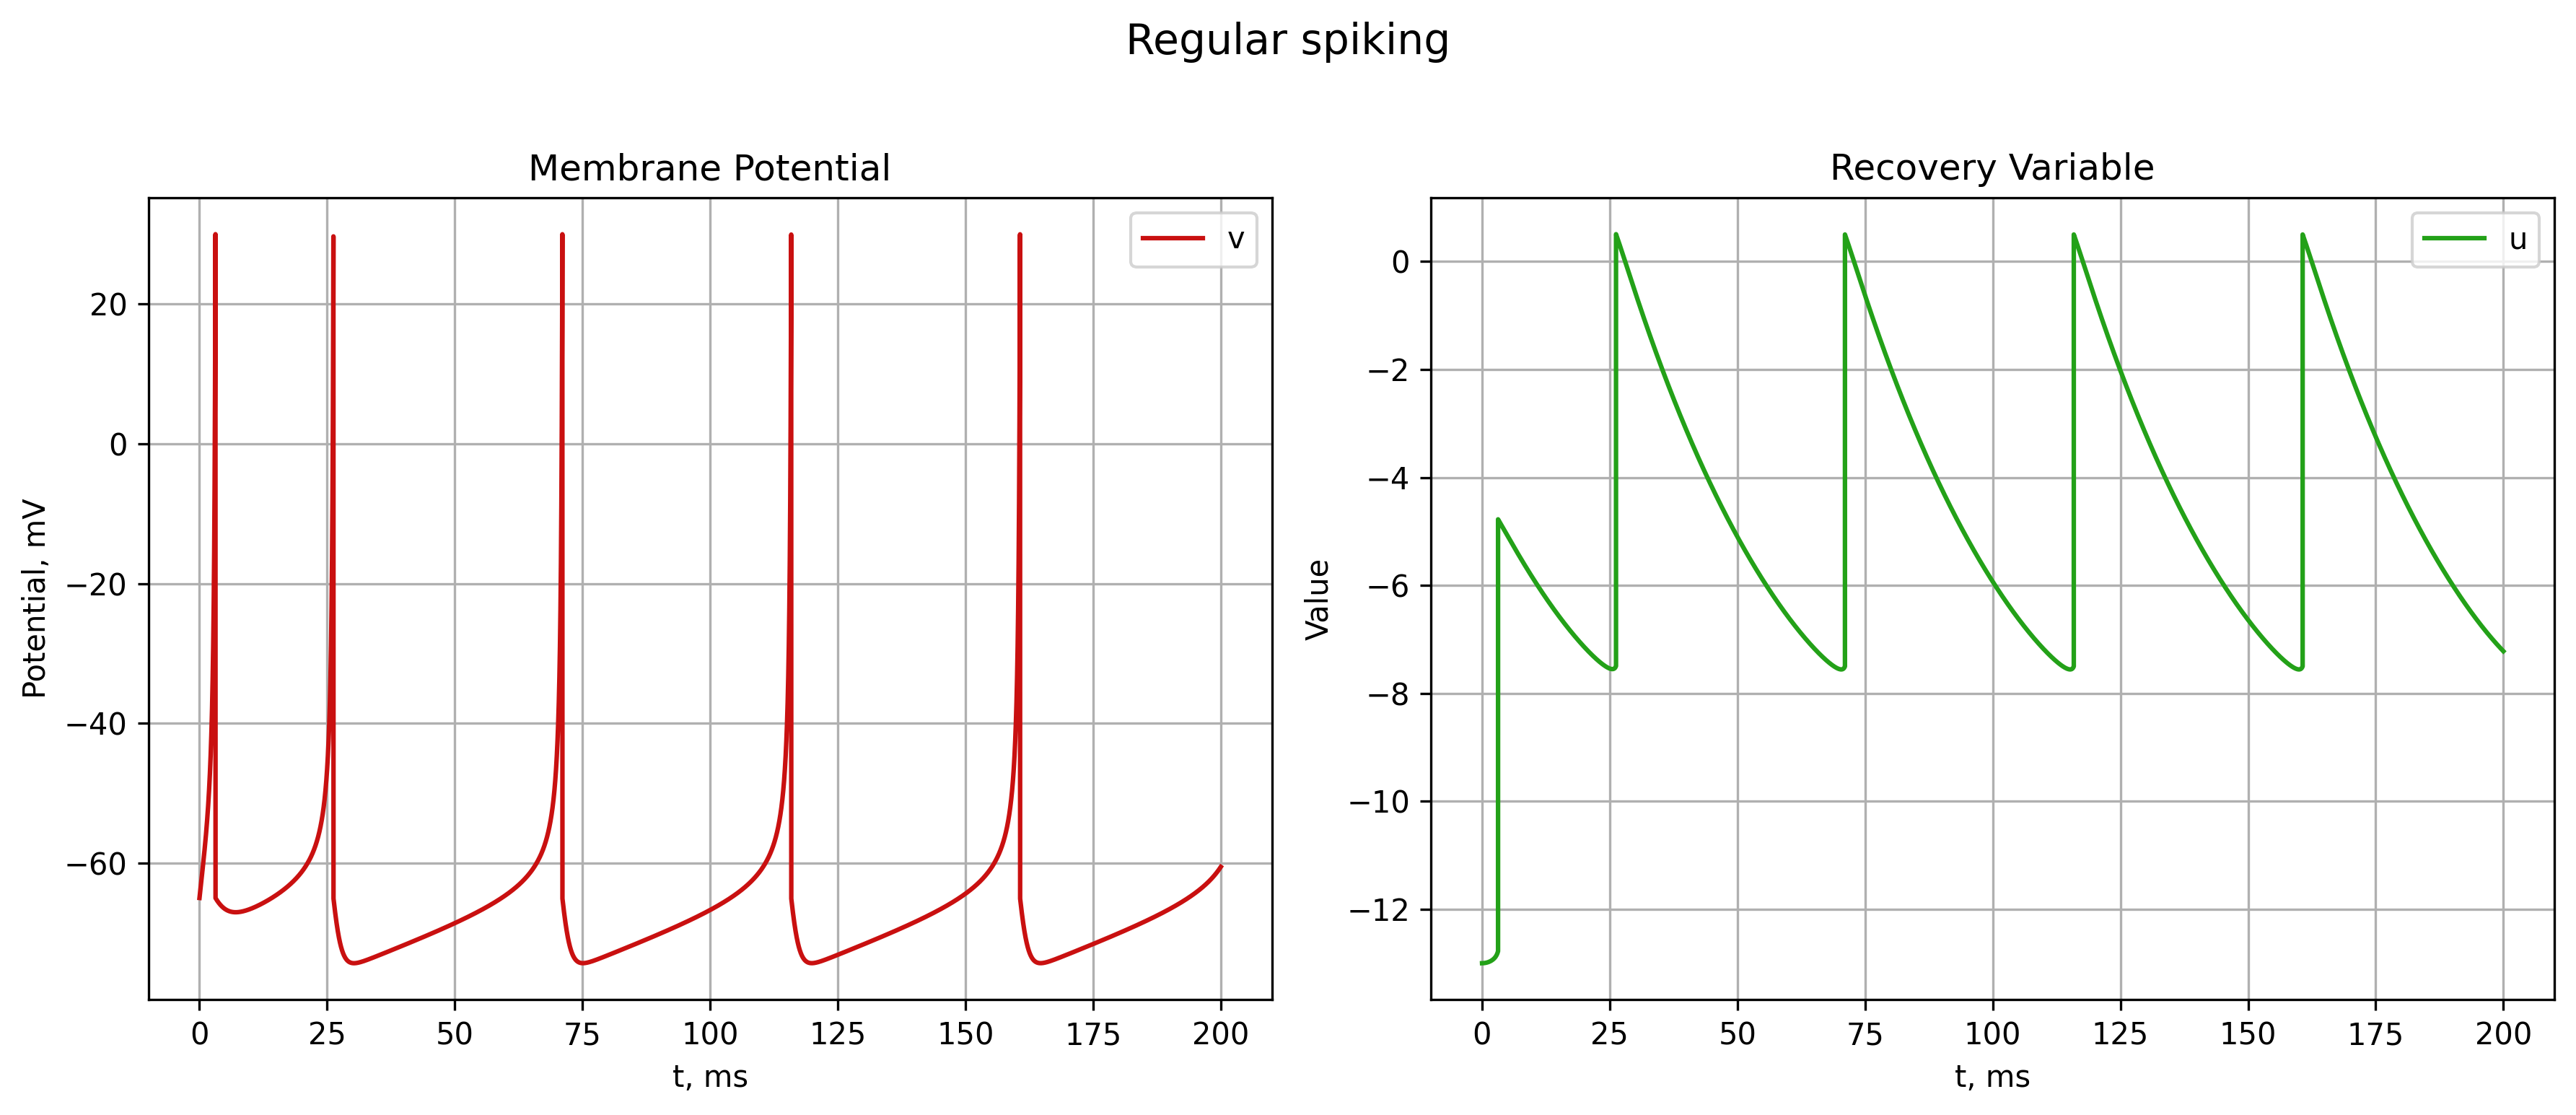
\includegraphics[width=1\linewidth]{pic/regular_spiking.png}}
\caption{Визуализация регулярно-спайкового нейрона при $I=10$ нА.}
\label{1_rs}
\end{figure}

\begin{figure}[h]
	\center{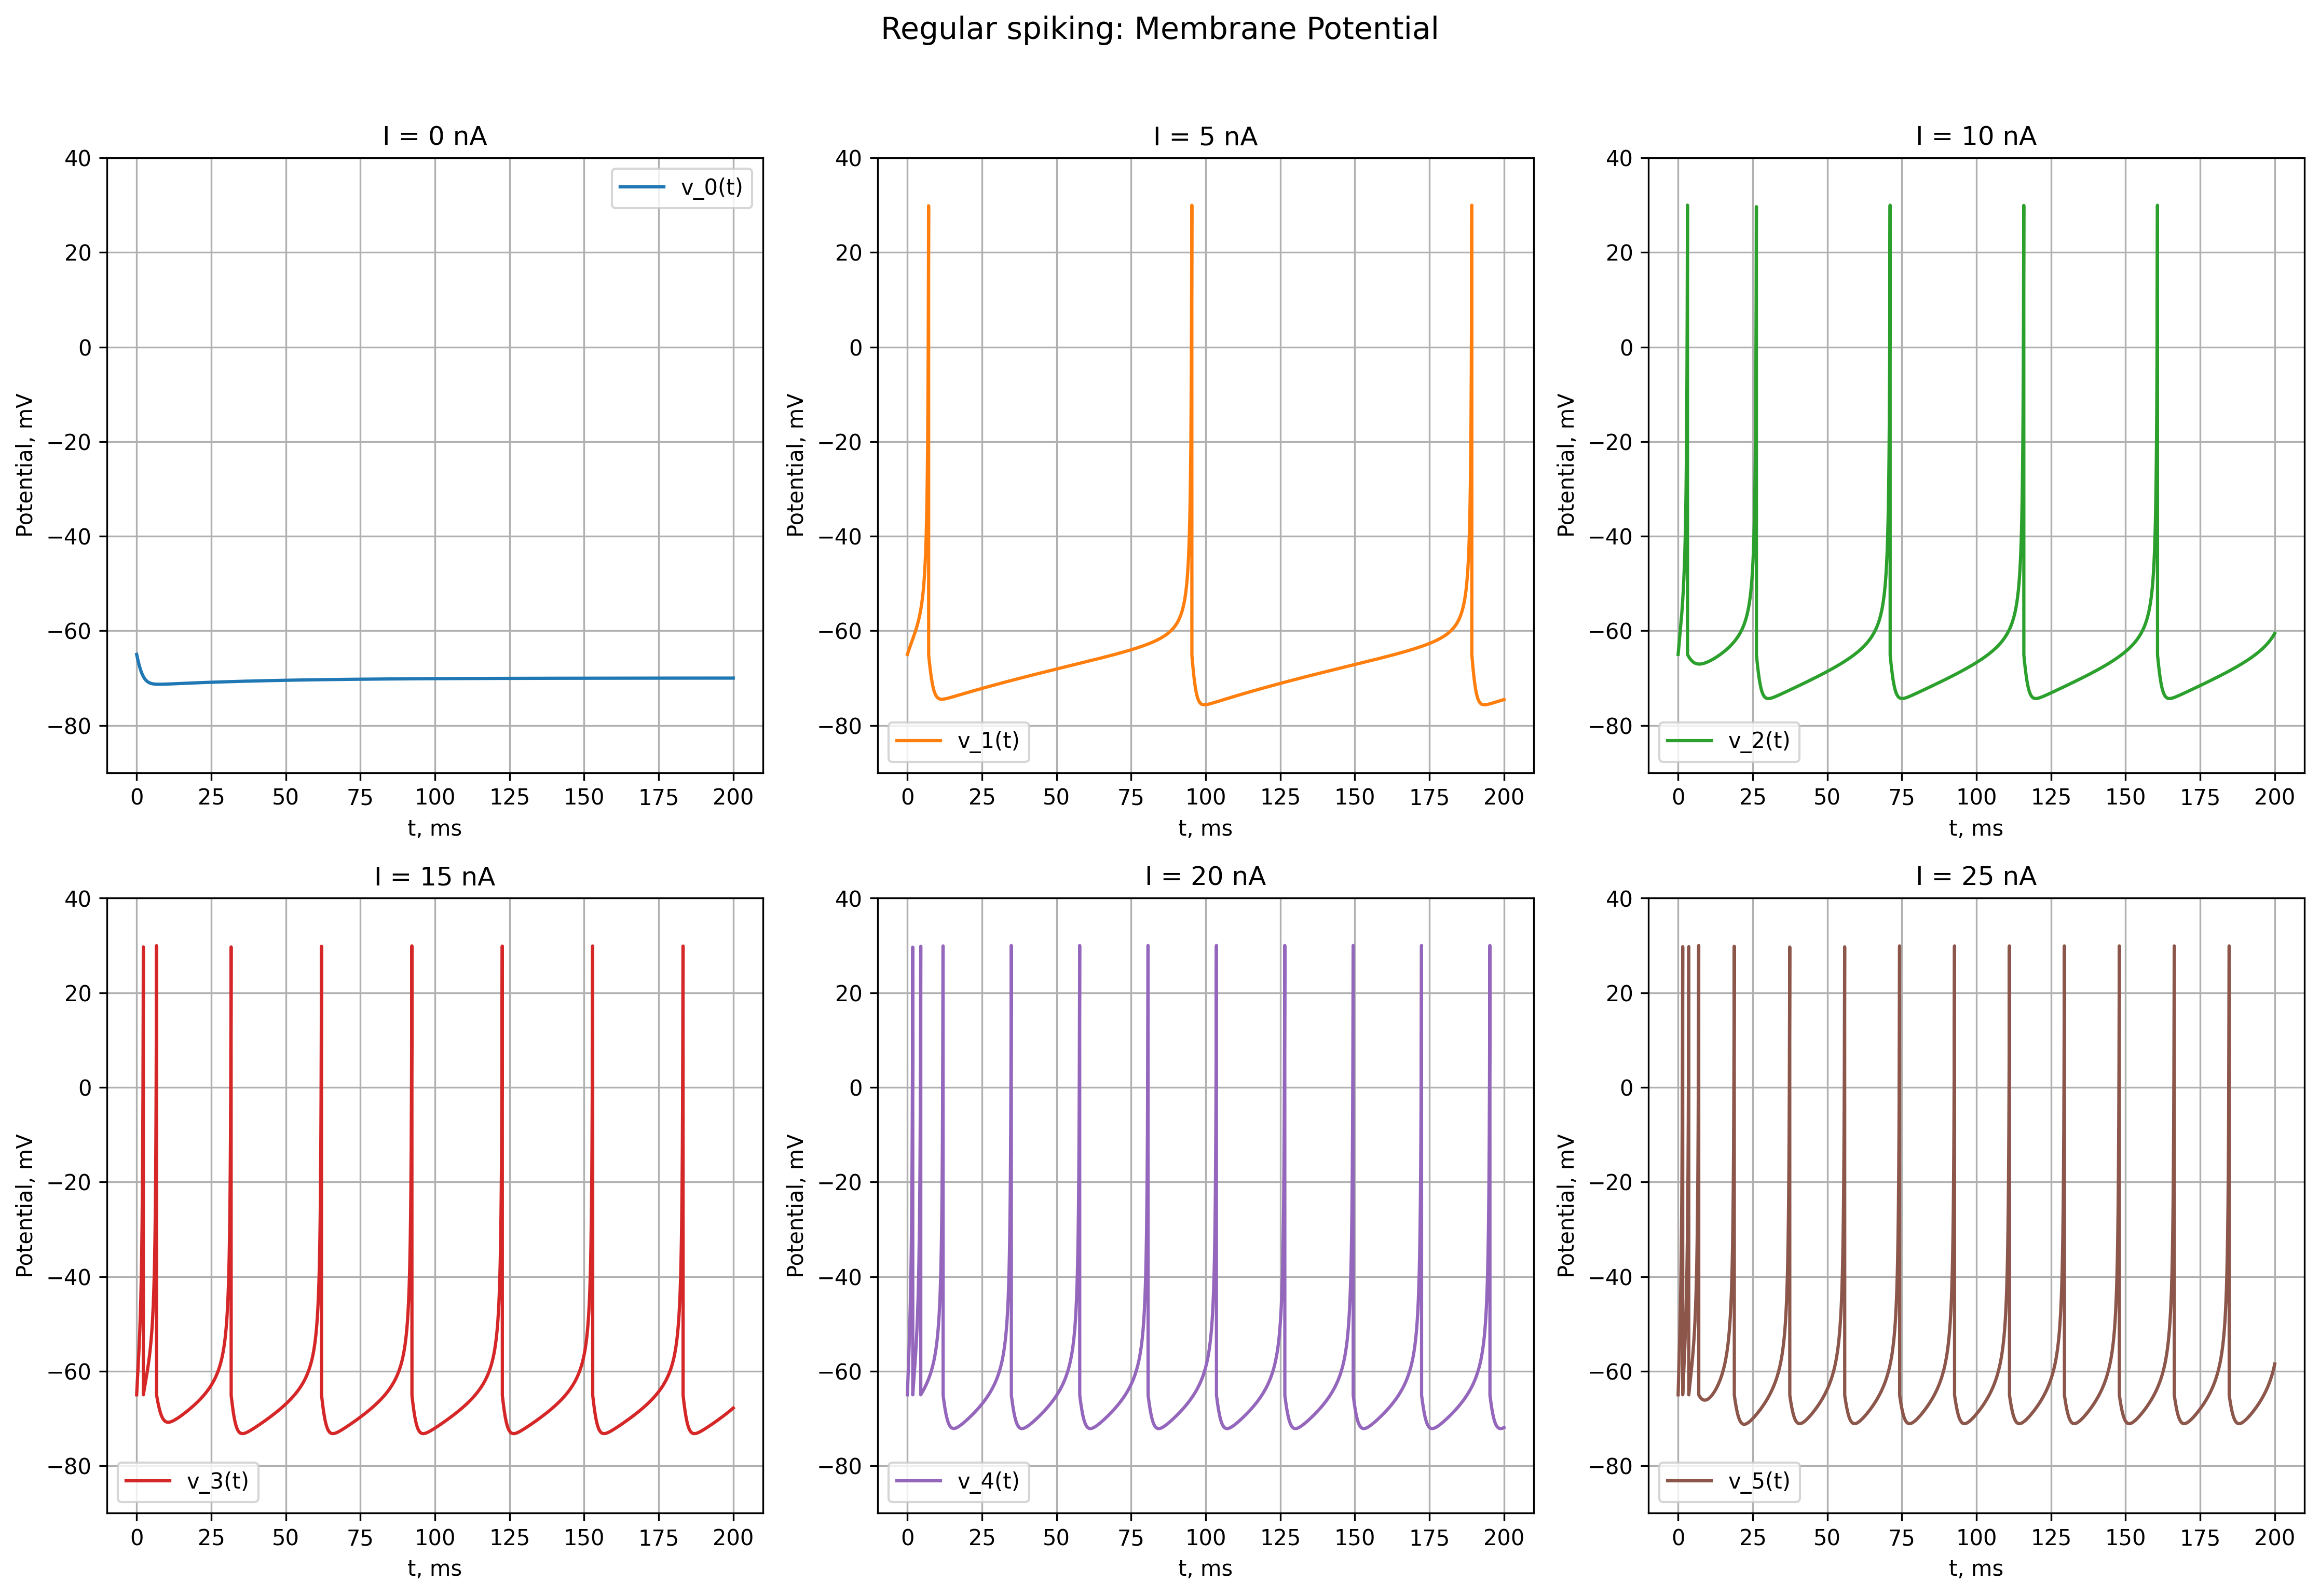
\includegraphics[width=1\linewidth]{pic/rs_different_I_potentials.png}}
	\caption{Визуализация $v(t)$ регулярно-спайкового нейрона для разных значений $I$.}
	\label{rs_different_I_potentials}
\end{figure}

\begin{figure}[h]
	\center{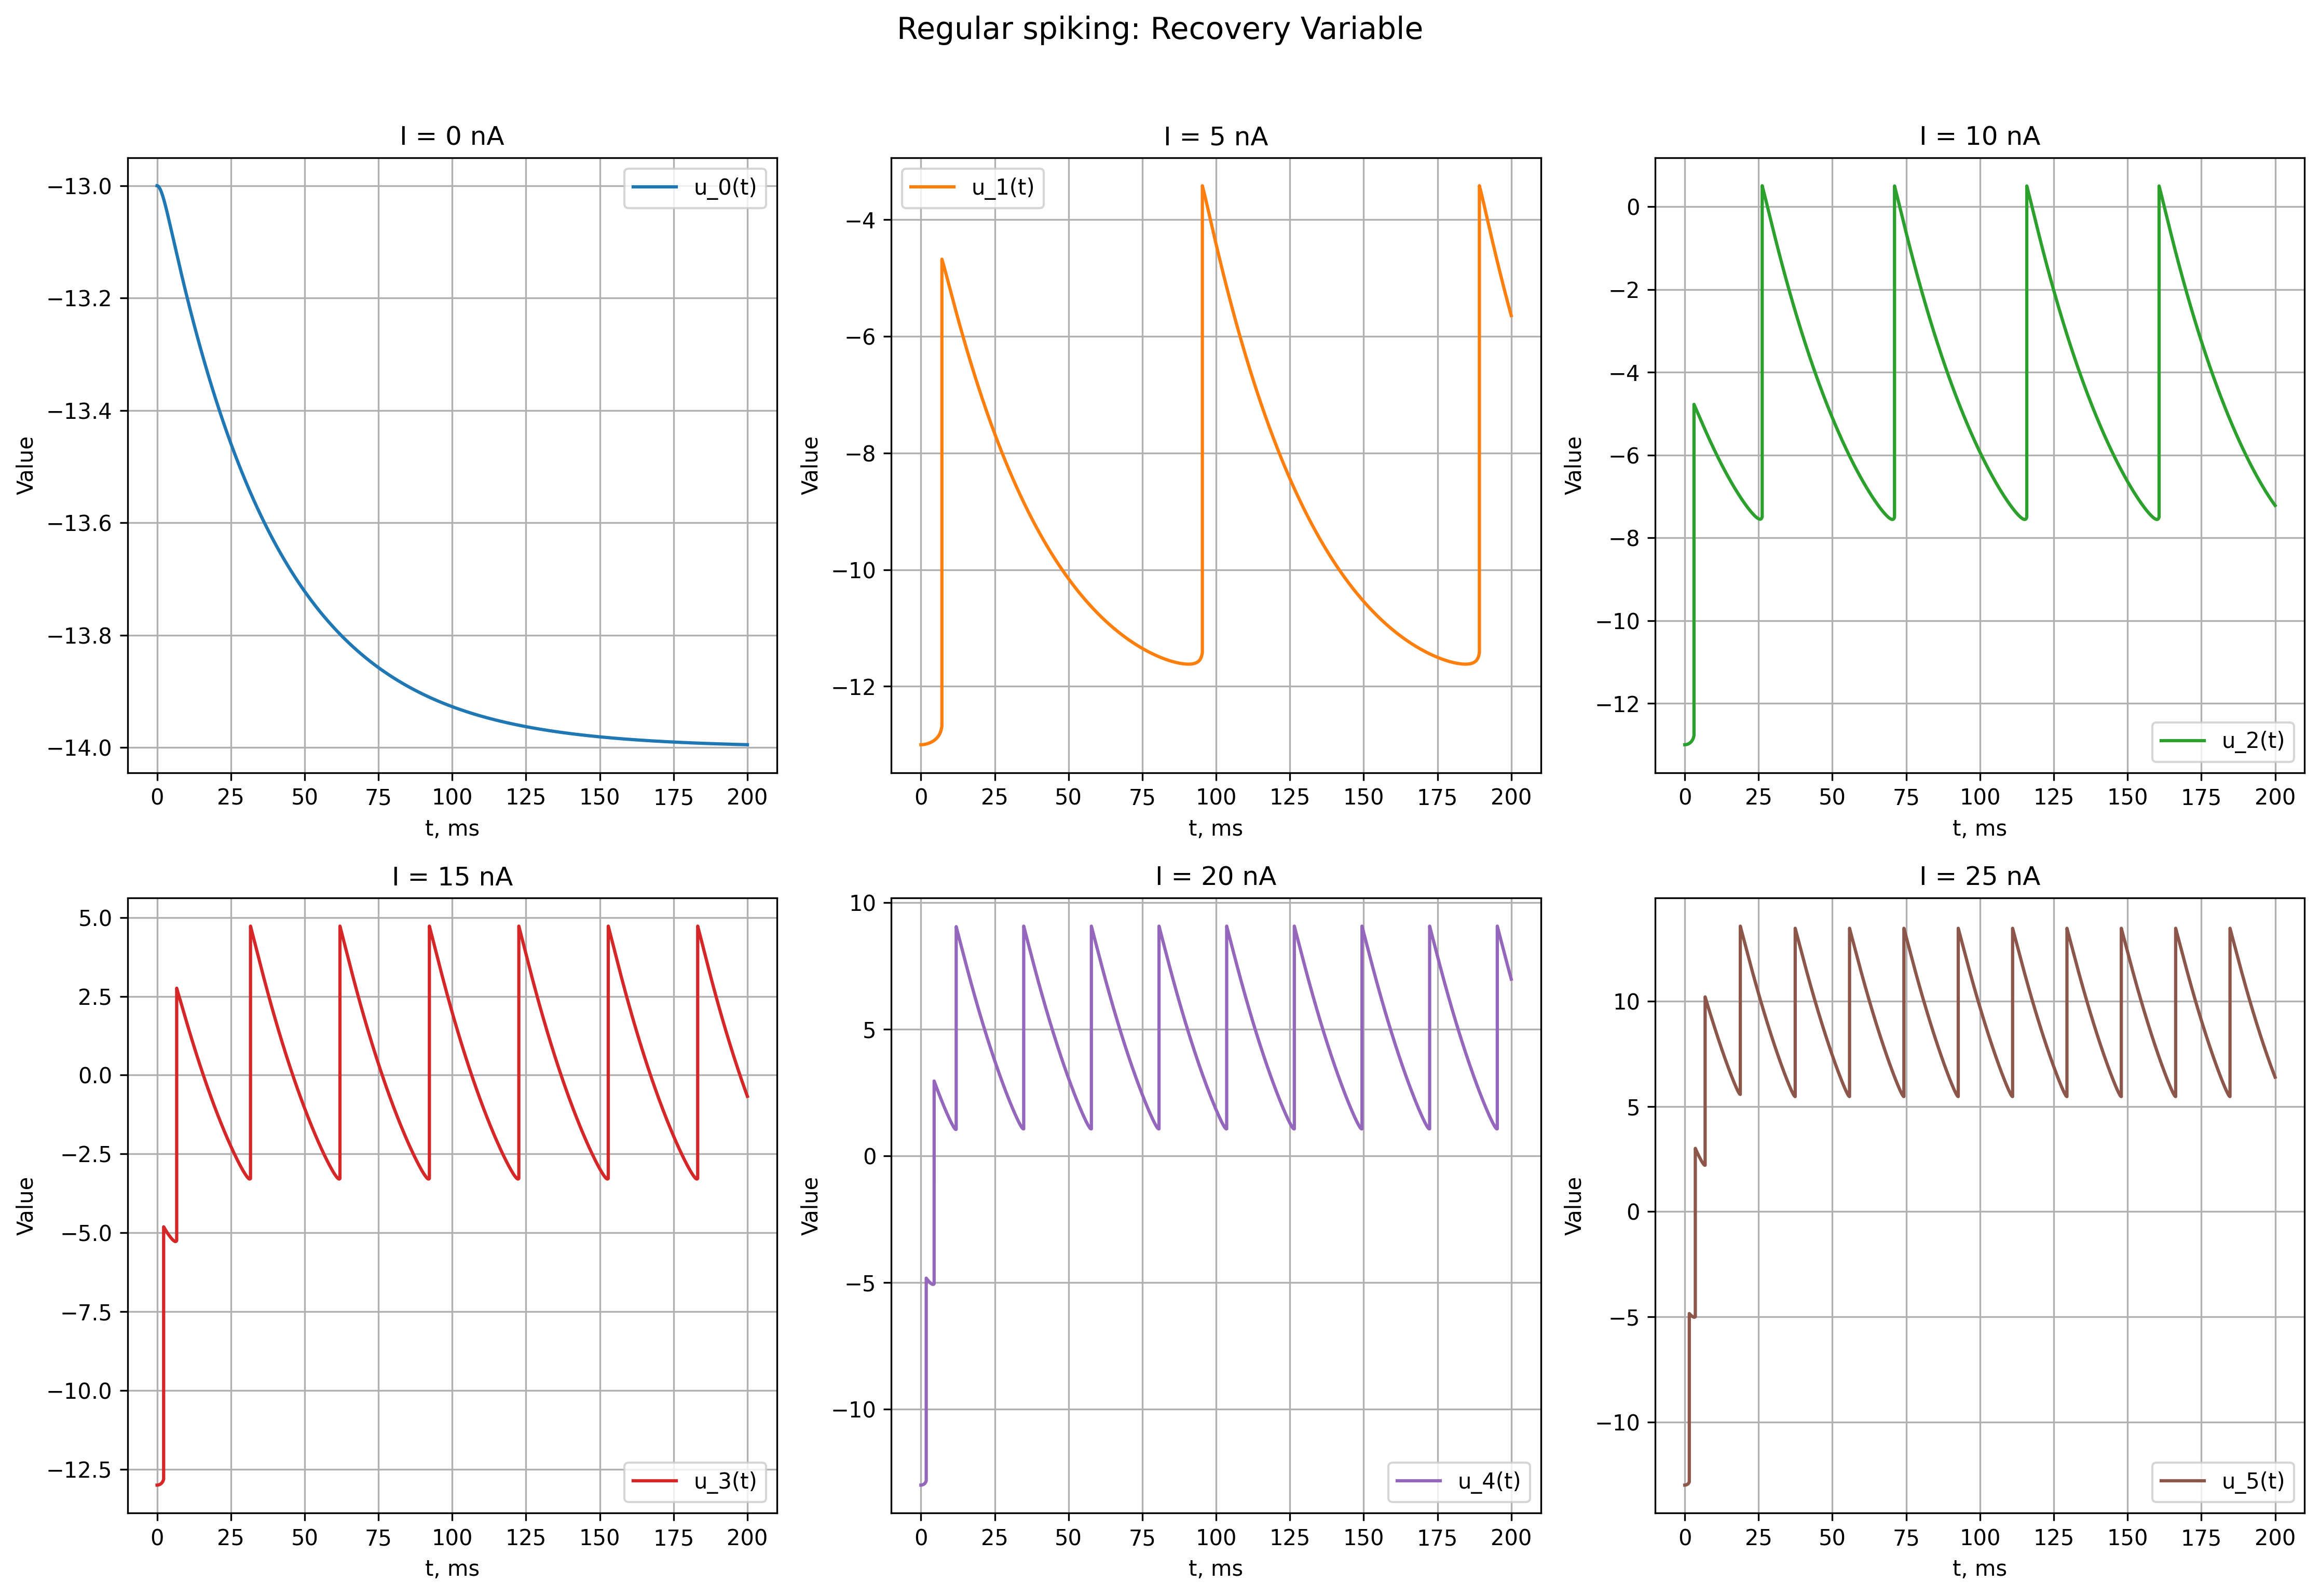
\includegraphics[width=1\linewidth]{pic/rs_different_I_recovery.png}}
	\caption{Визуализация $u(t)$ регулярно-спайкового нейрона для разных значений $I$.}
	\label{rs_different_I_recovery}
\end{figure}

\begin{figure}[h]
\center{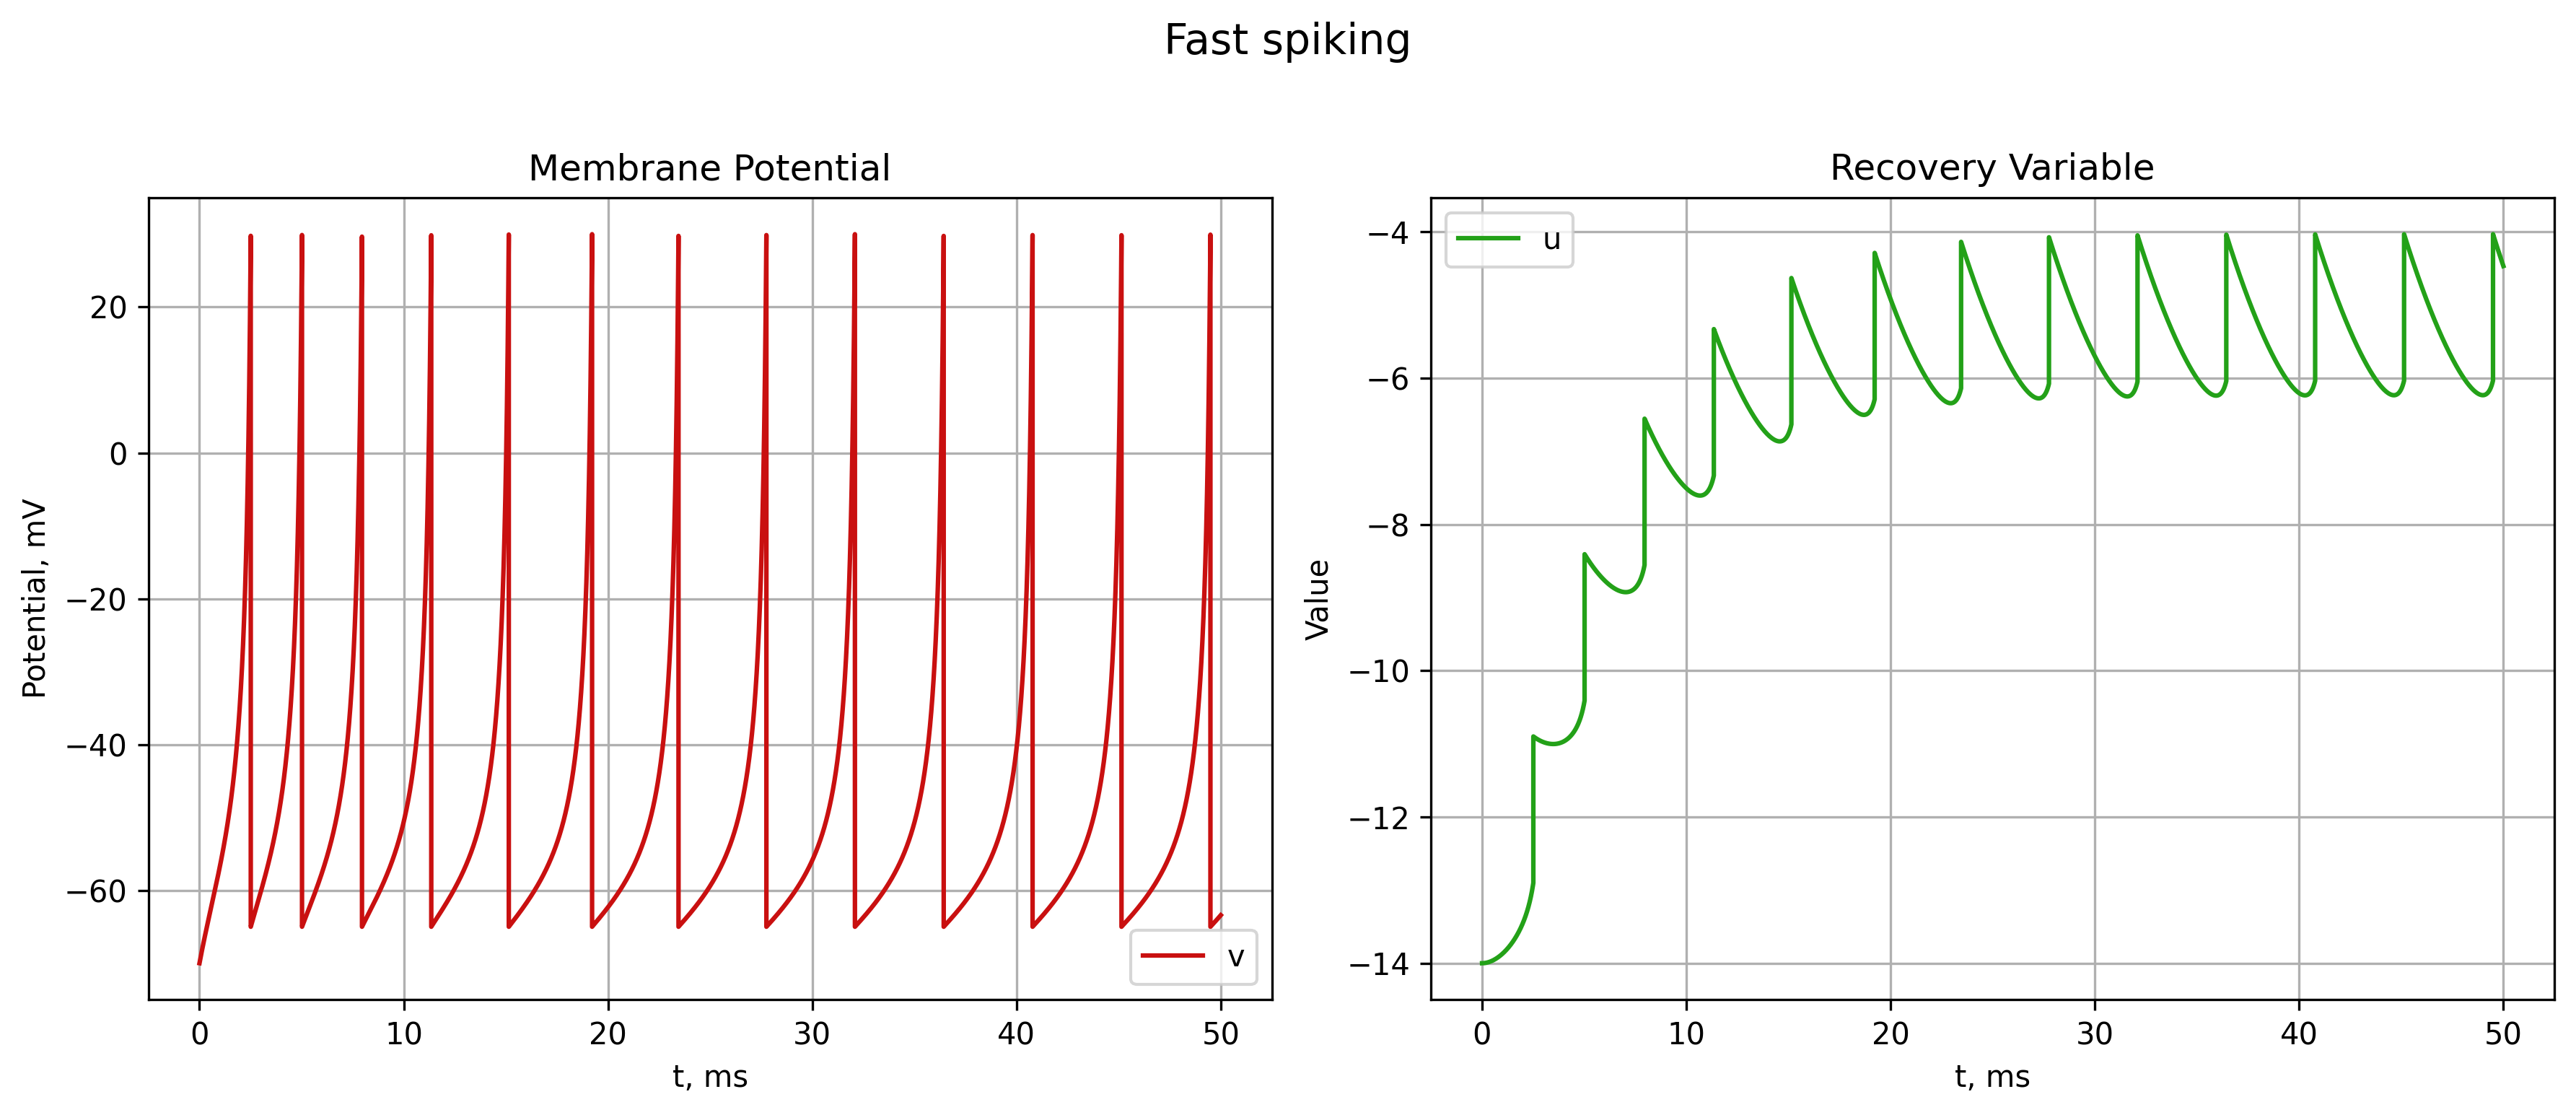
\includegraphics[width=1\linewidth]{pic/fast_spiking.png}}
\caption{Визуализация быстро-спайкового нейрона при $I=15$ нА.}
\label{1_fs}
\end{figure}

\begin{figure}[h]
	\center{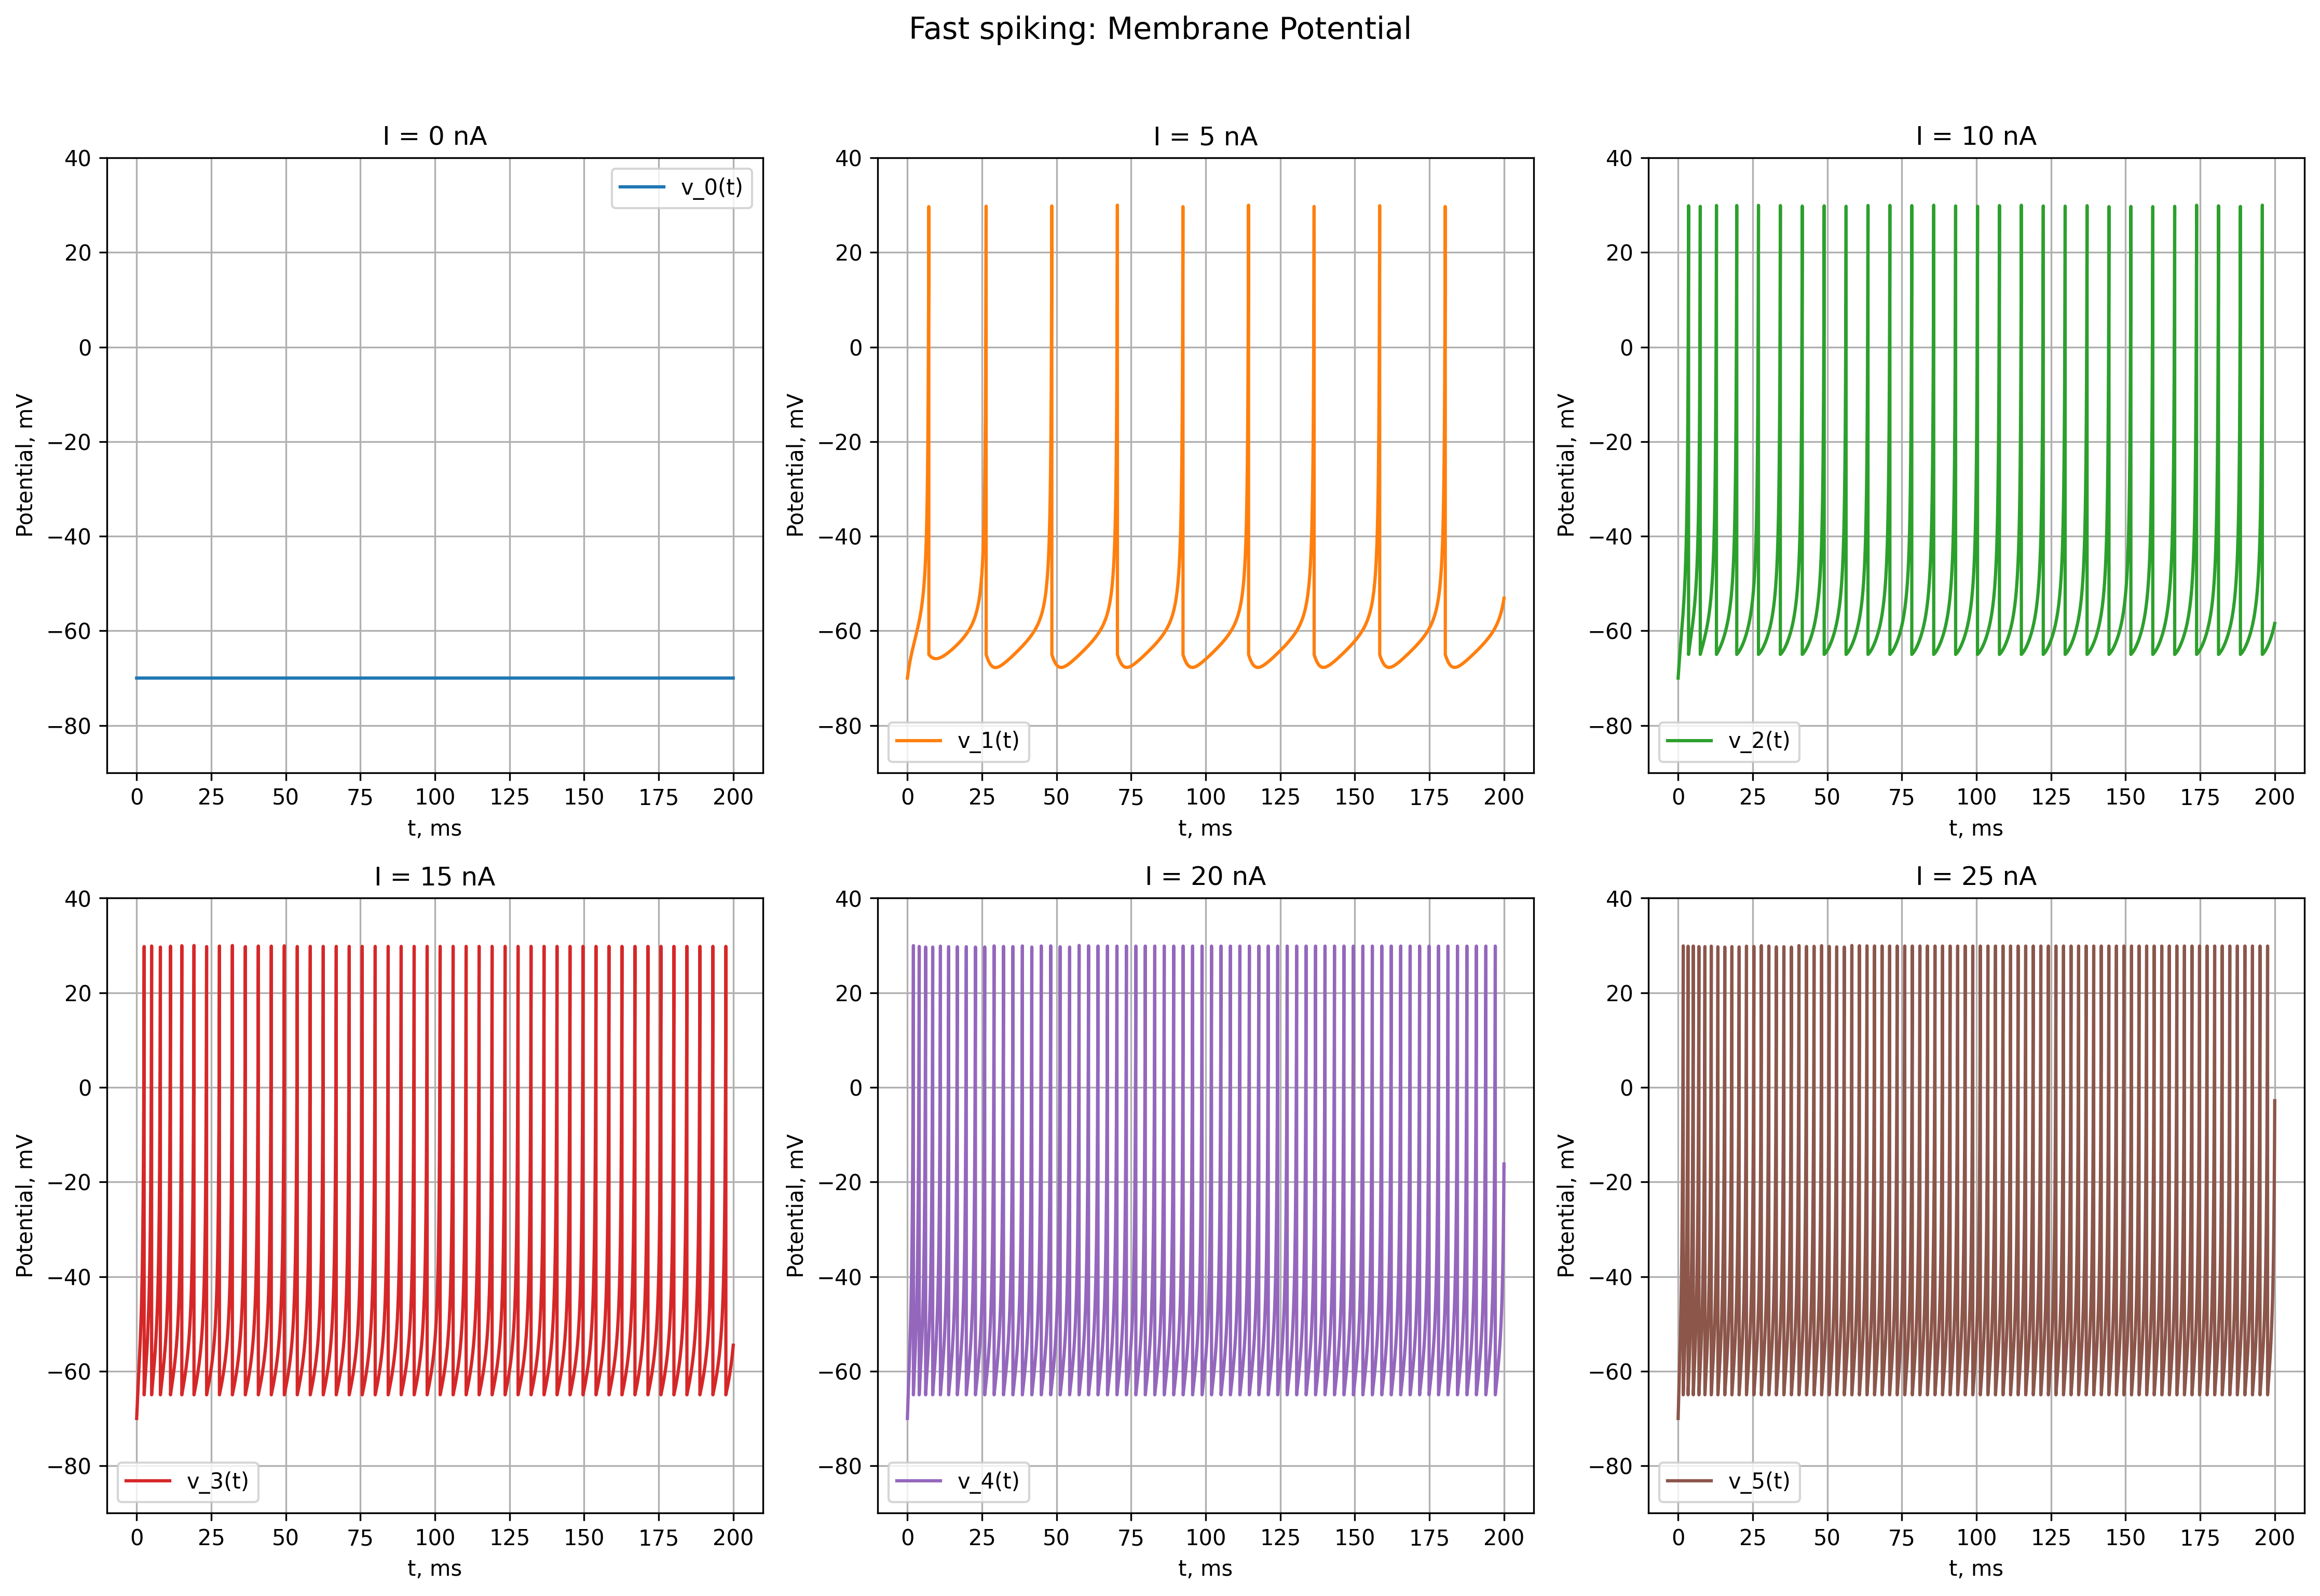
\includegraphics[width=1\linewidth]{pic/fs_different_I_potentials.png}}
	\caption{Визуализация $v(t)$ быстро-спайкового нейрона для разных значений $I$.}
	\label{fs_different_I_potentials}
\end{figure}

\begin{figure}[h]
	\center{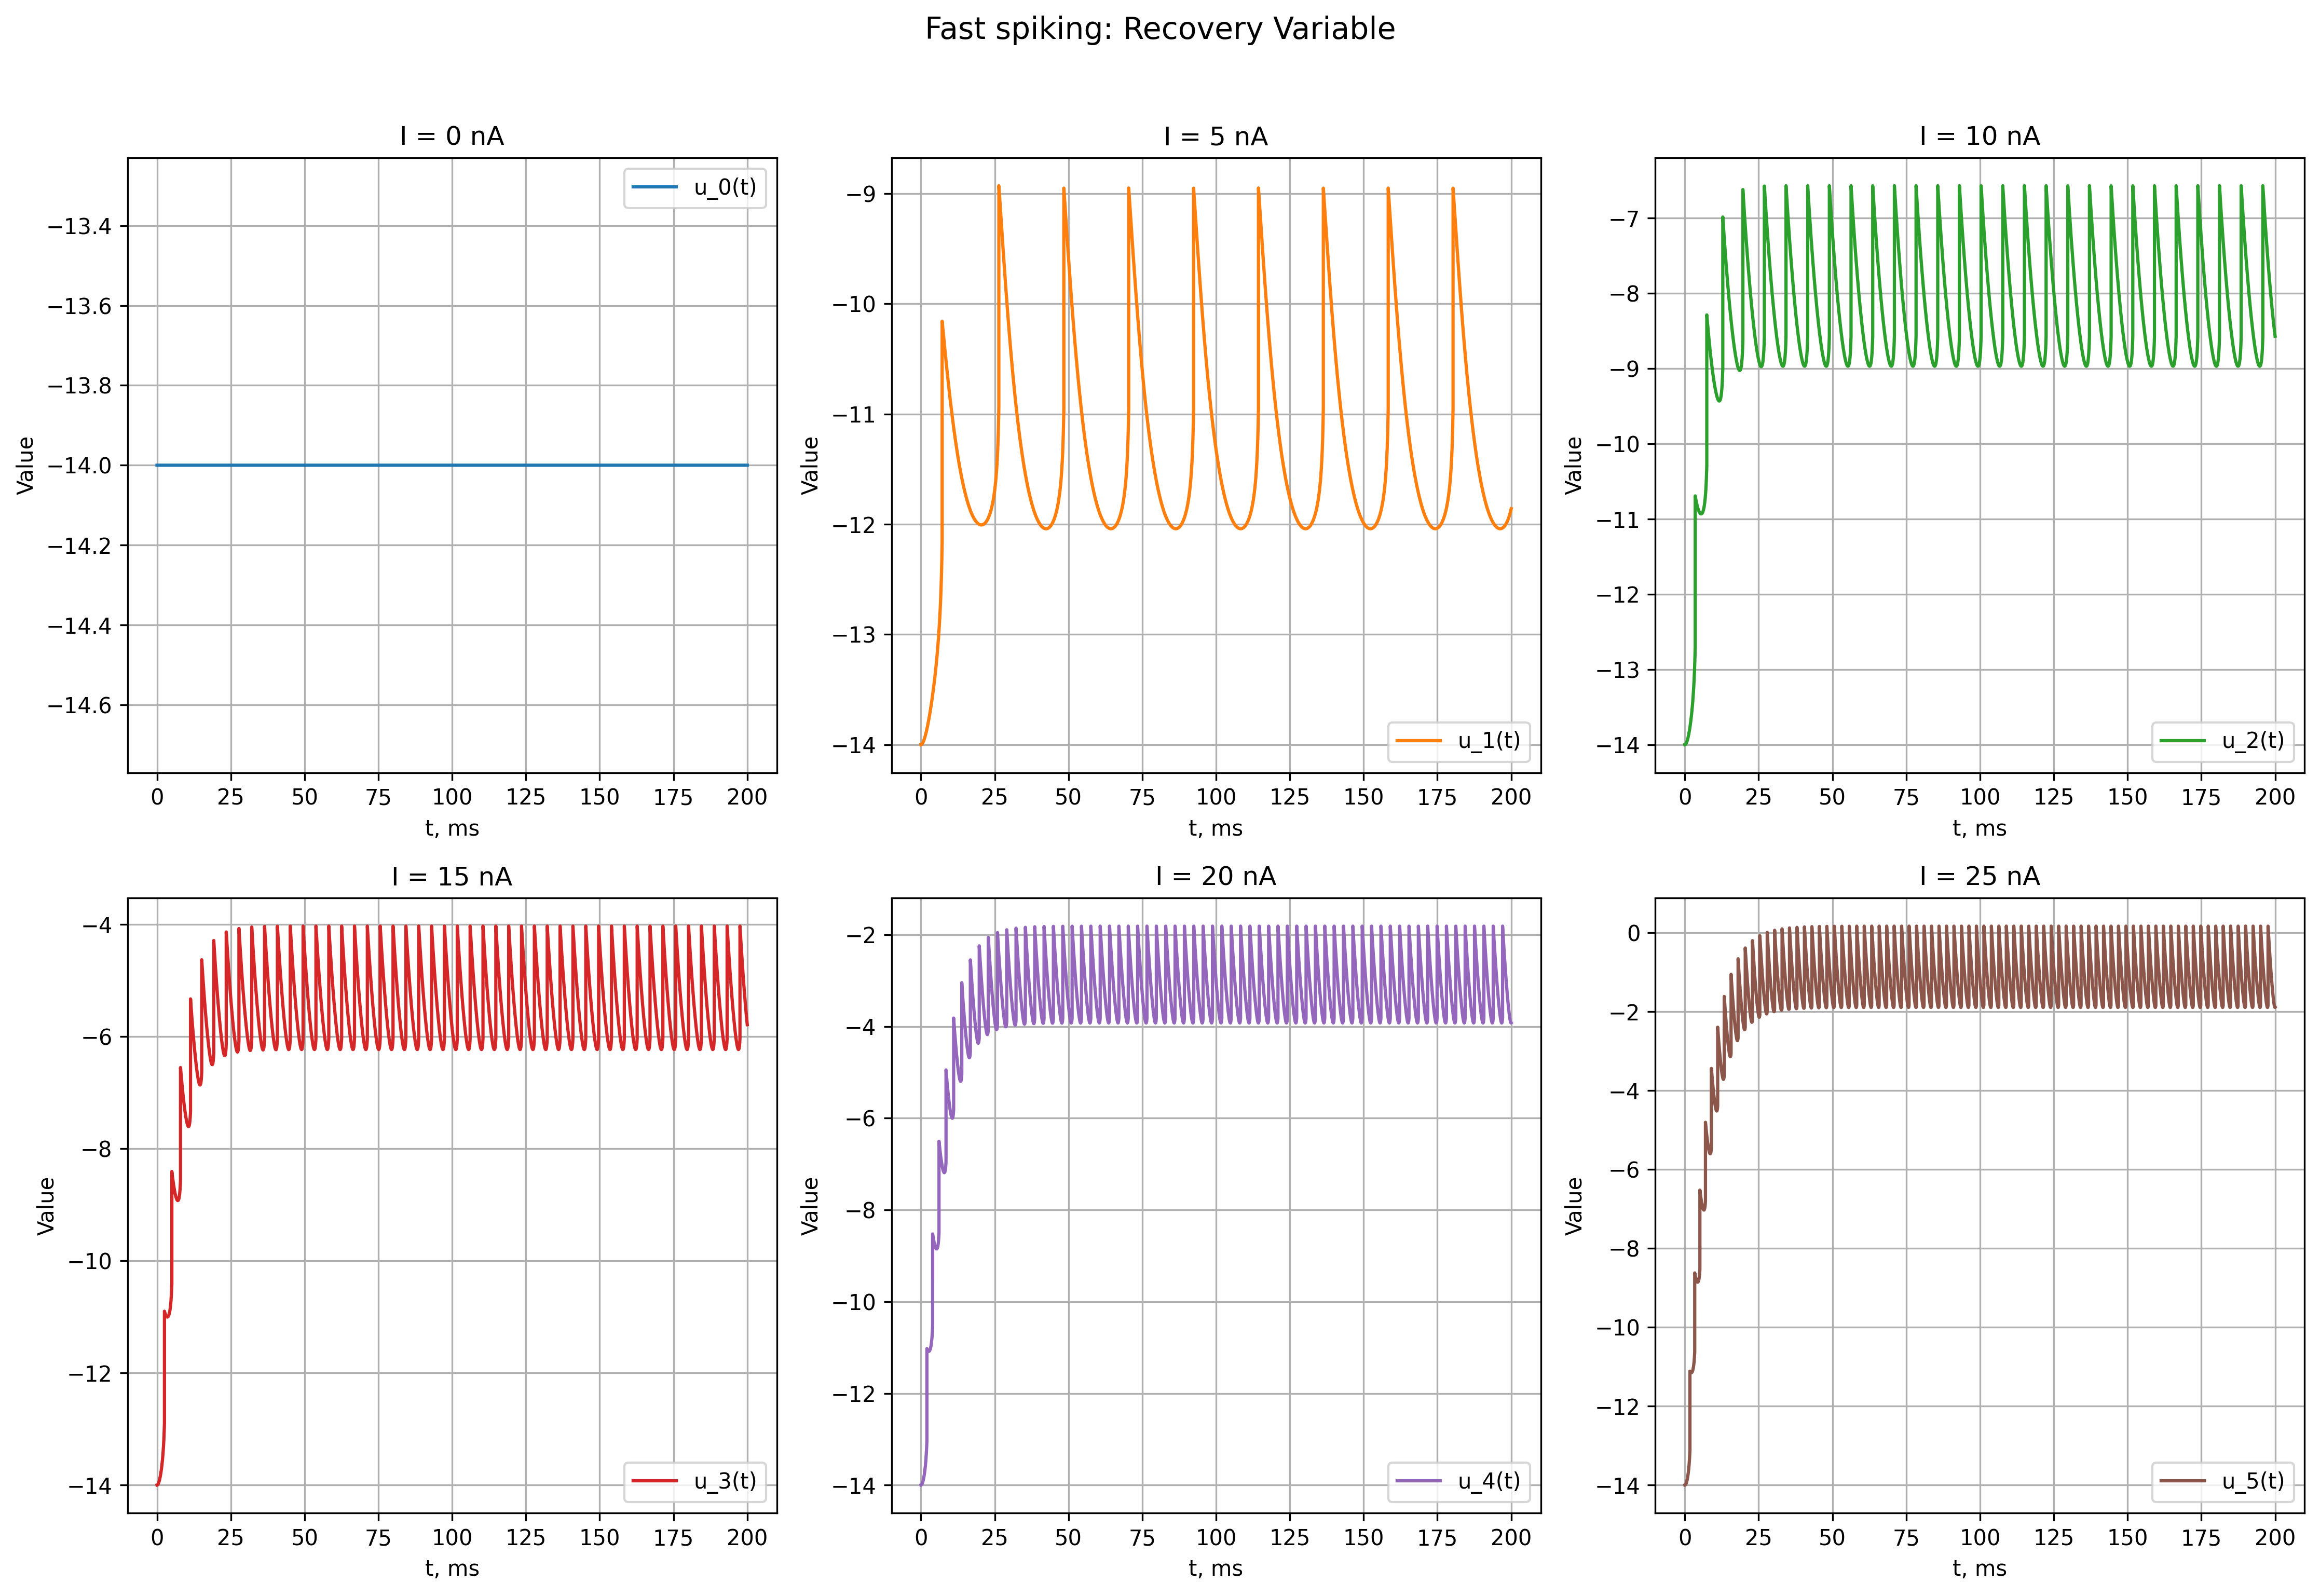
\includegraphics[width=1\linewidth]{pic/fs_different_I_recovery.png}}
	\caption{Визуализация $u(t)$ быстро-спайкового нейрона для разных значений $I$.}
	\label{fs_different_I_recovery}
\end{figure}

\begin{figure}[h]
\center{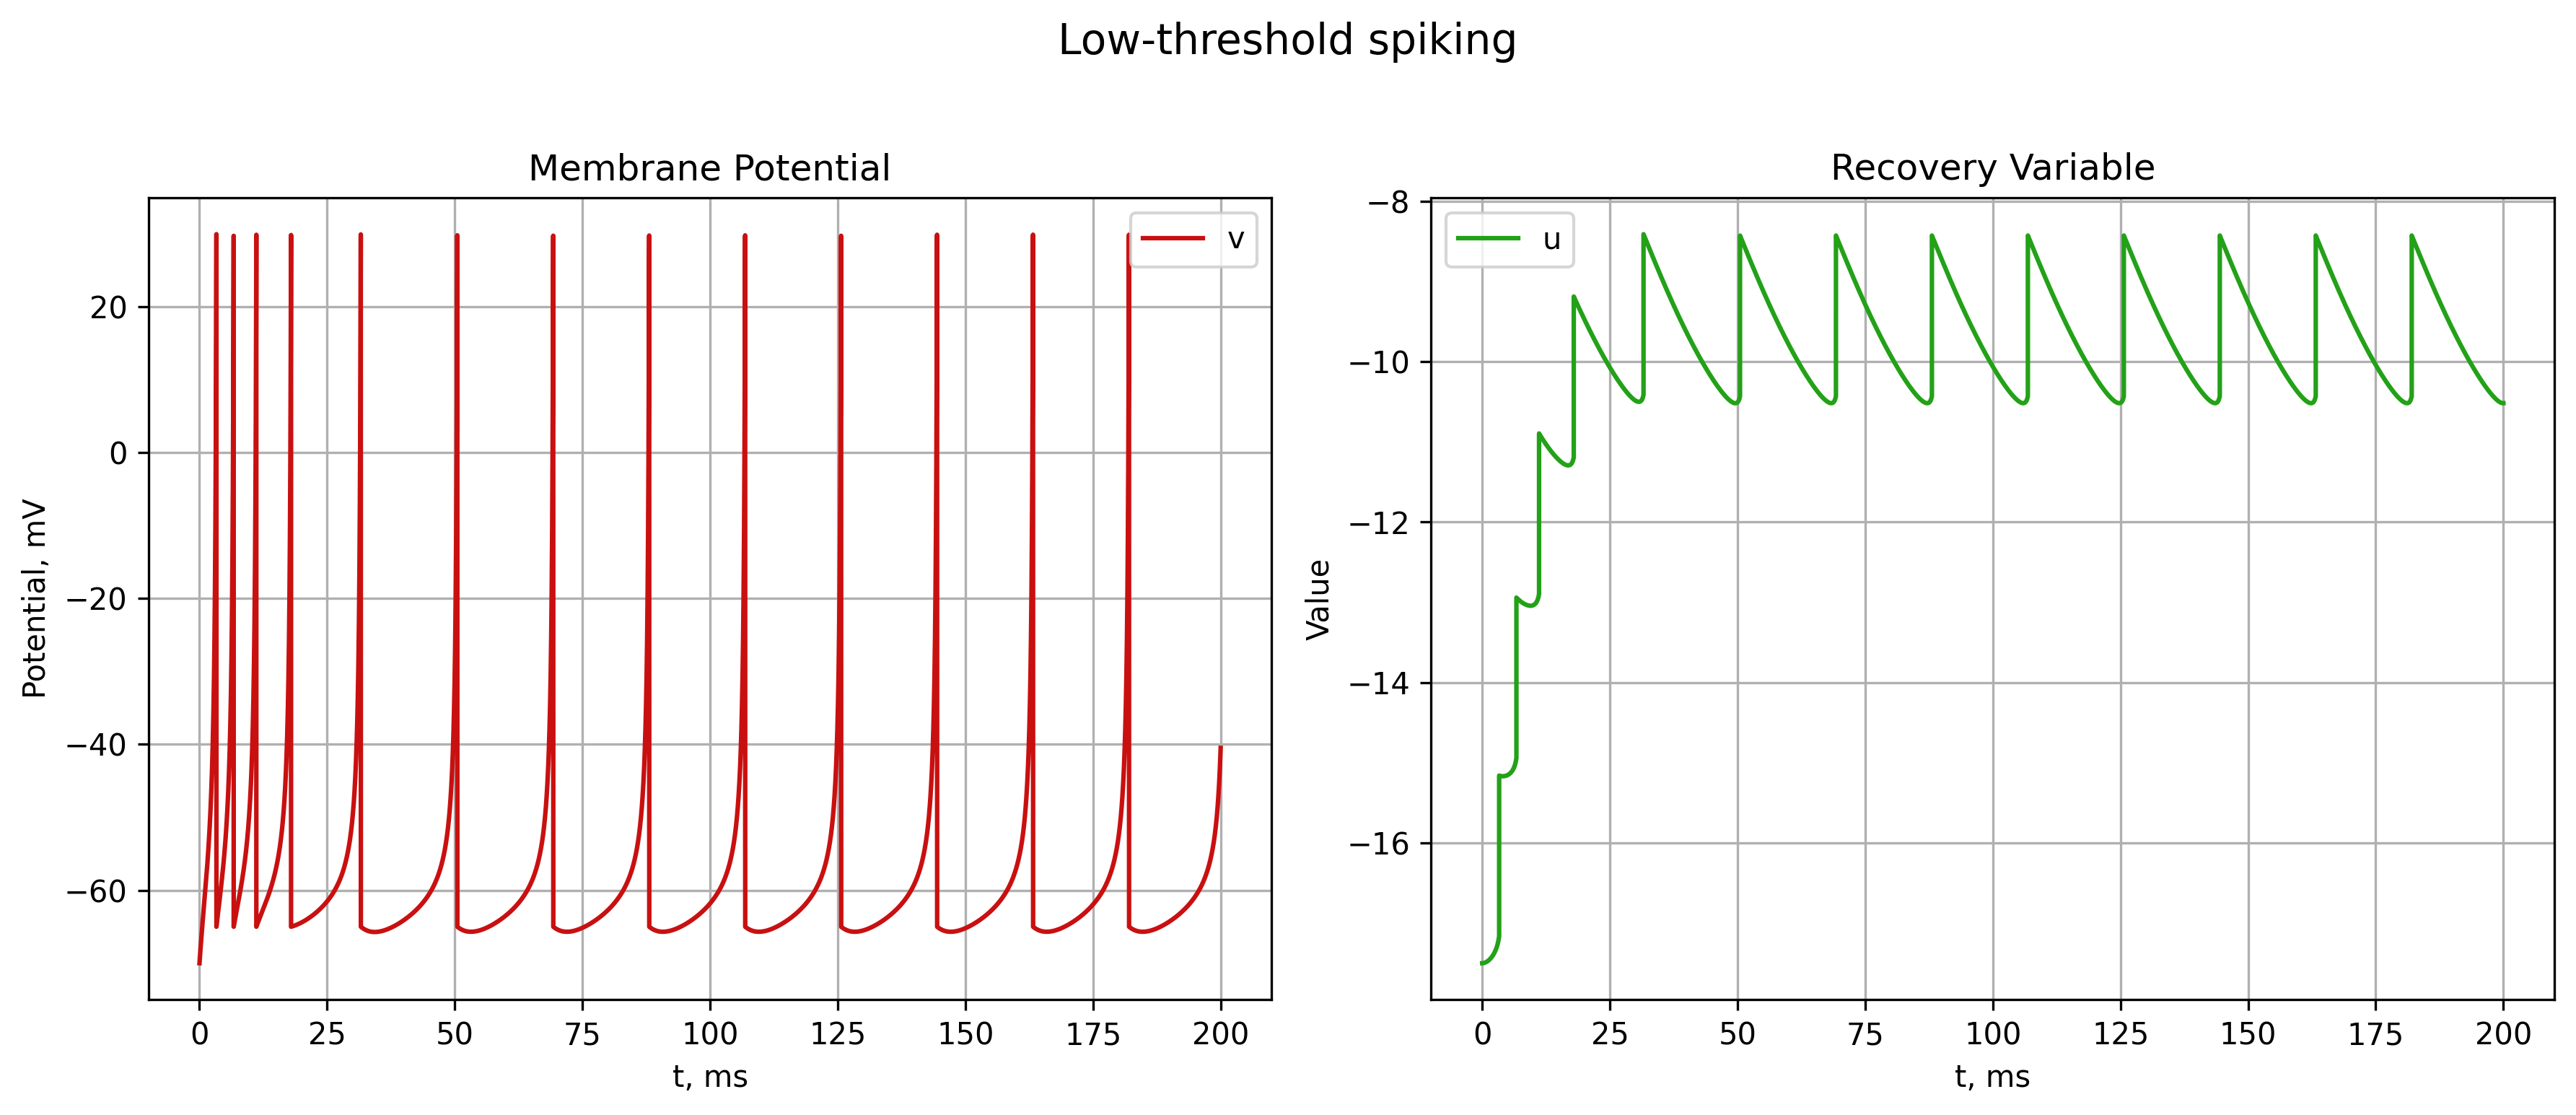
\includegraphics[width=1\linewidth]{pic/low_threshold_spiking.png}}
\caption{Визуализация низкопорогового спайкового нейрона при $I=7$ нА.}
\label{1_lts}
\end{figure}

\begin{figure}[h]
	\center{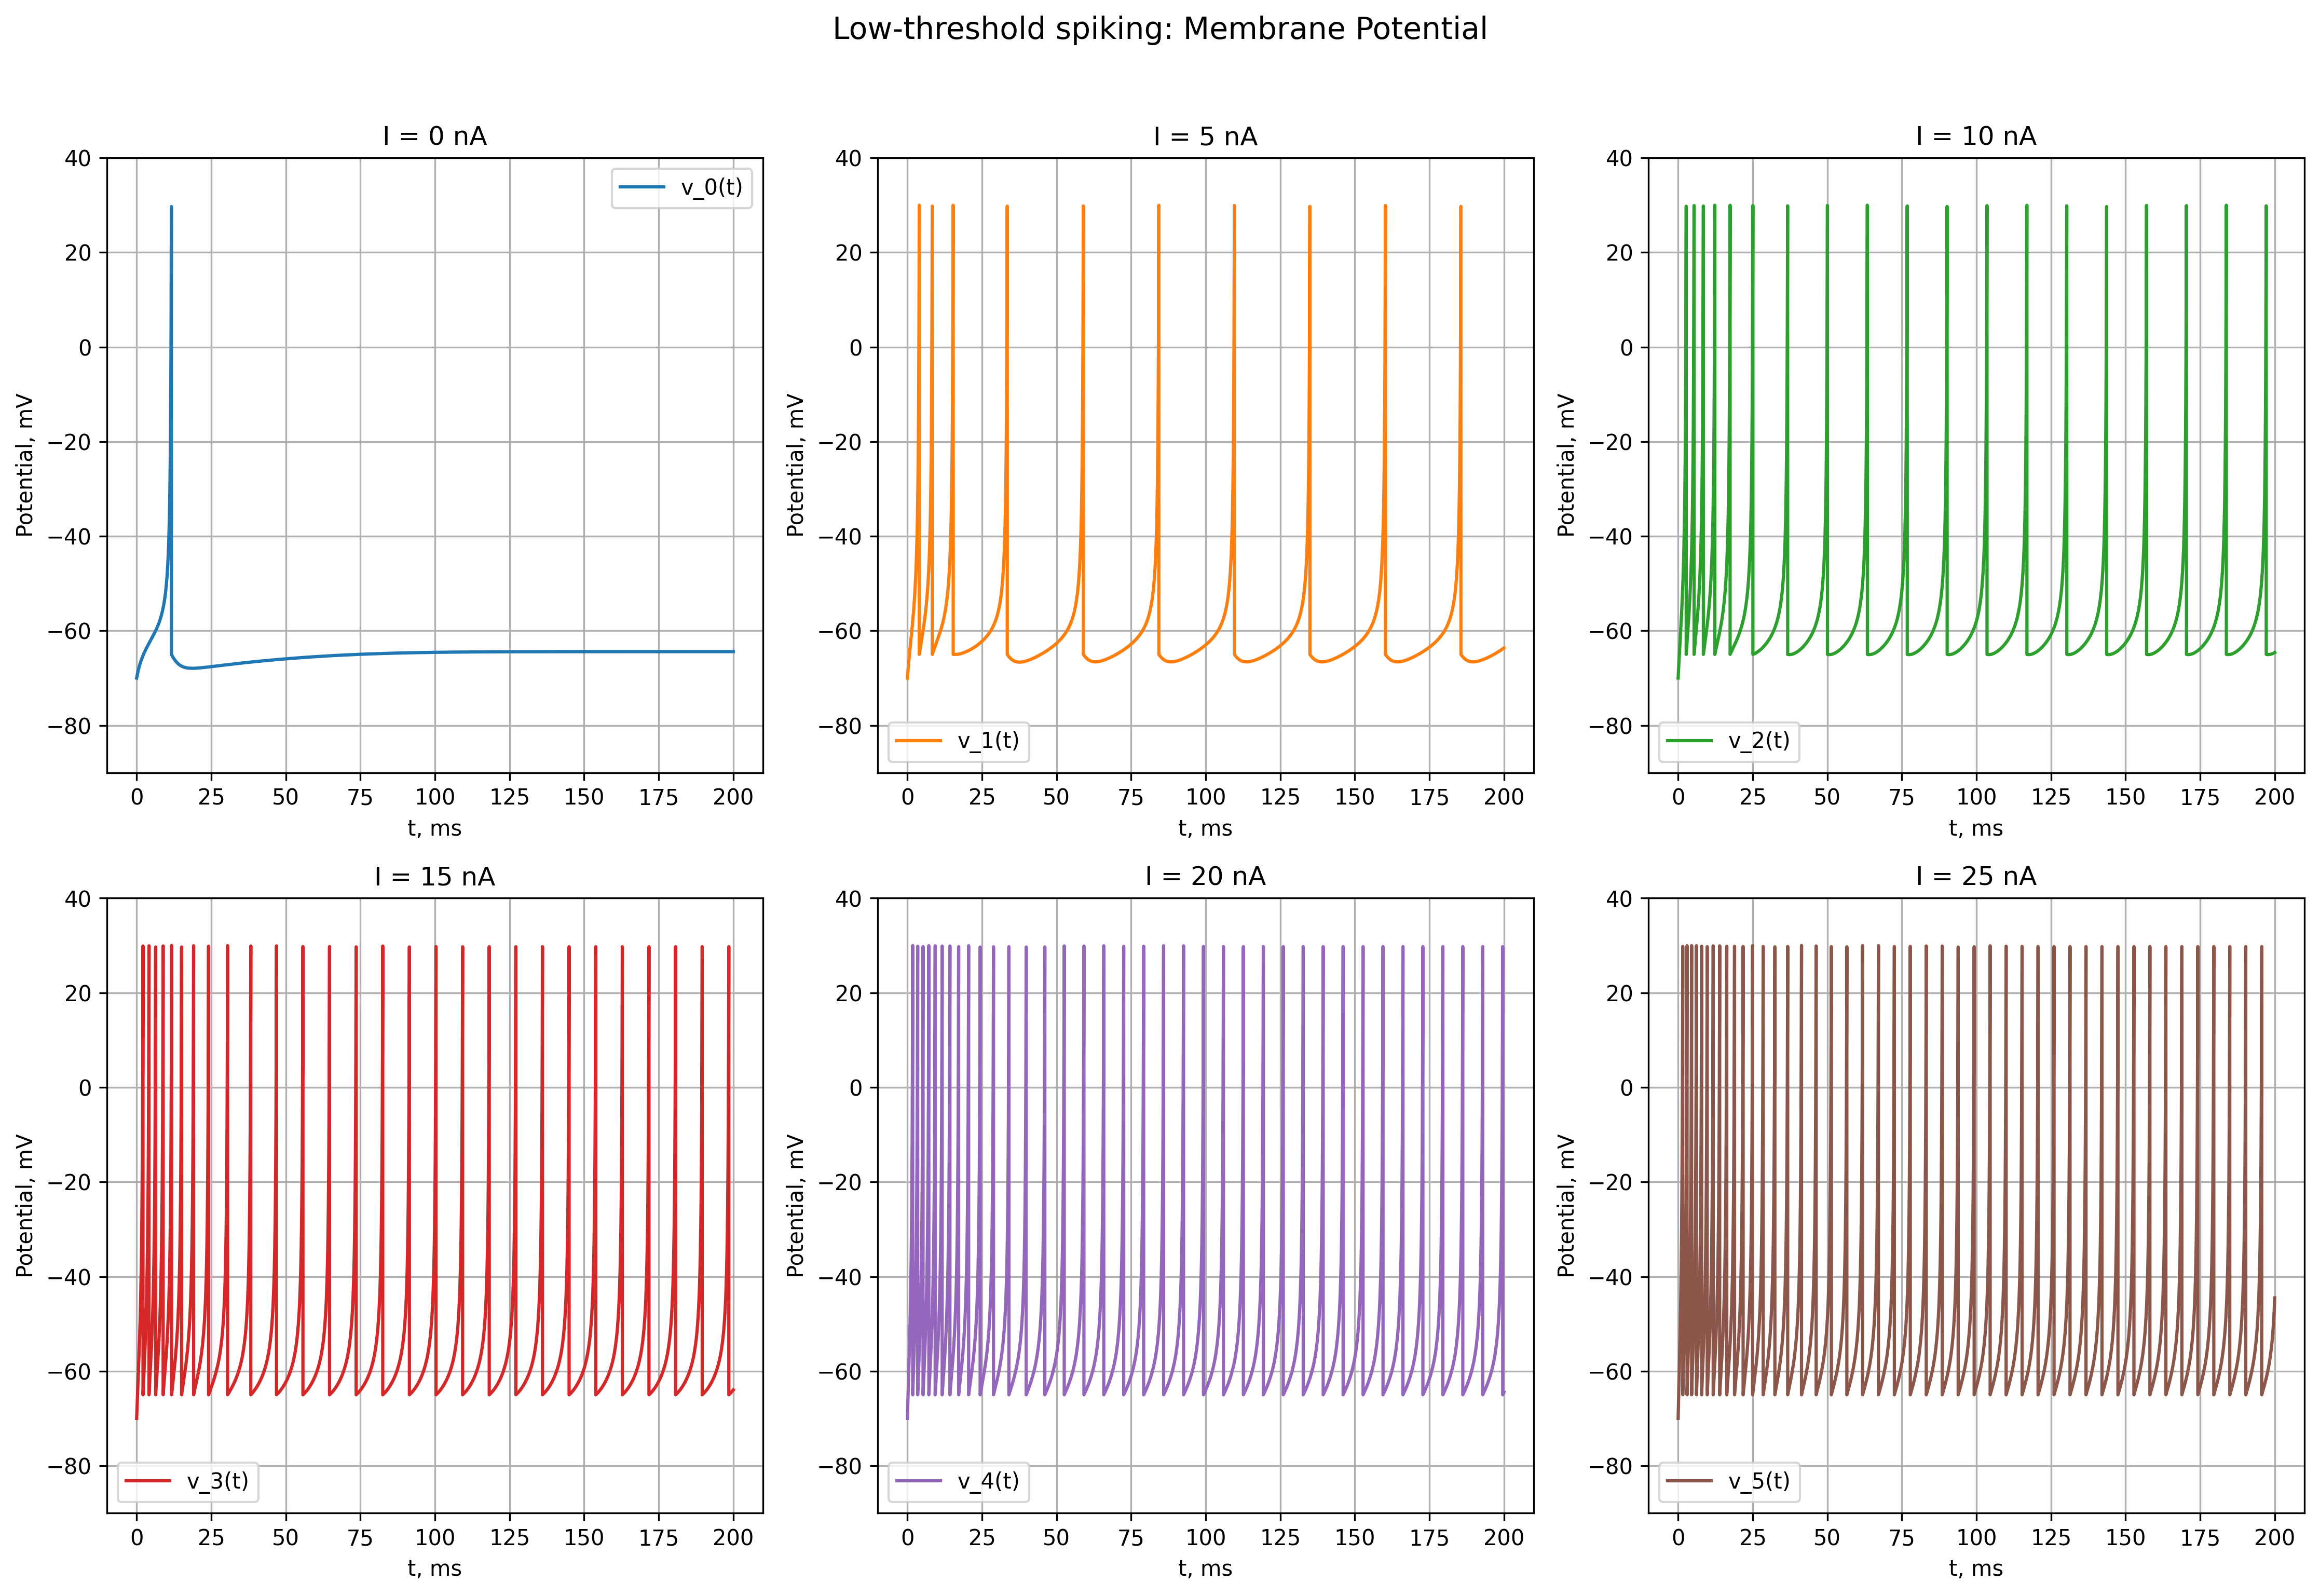
\includegraphics[width=1\linewidth]{pic/lts_different_I_potentials.png}}
	\caption{Визуализация $v(t)$ низкопорогового спайкового нейрона для разных значений $I$.}
	\label{lts_different_I_potentials}
\end{figure}

\begin{figure}[h]
	\center{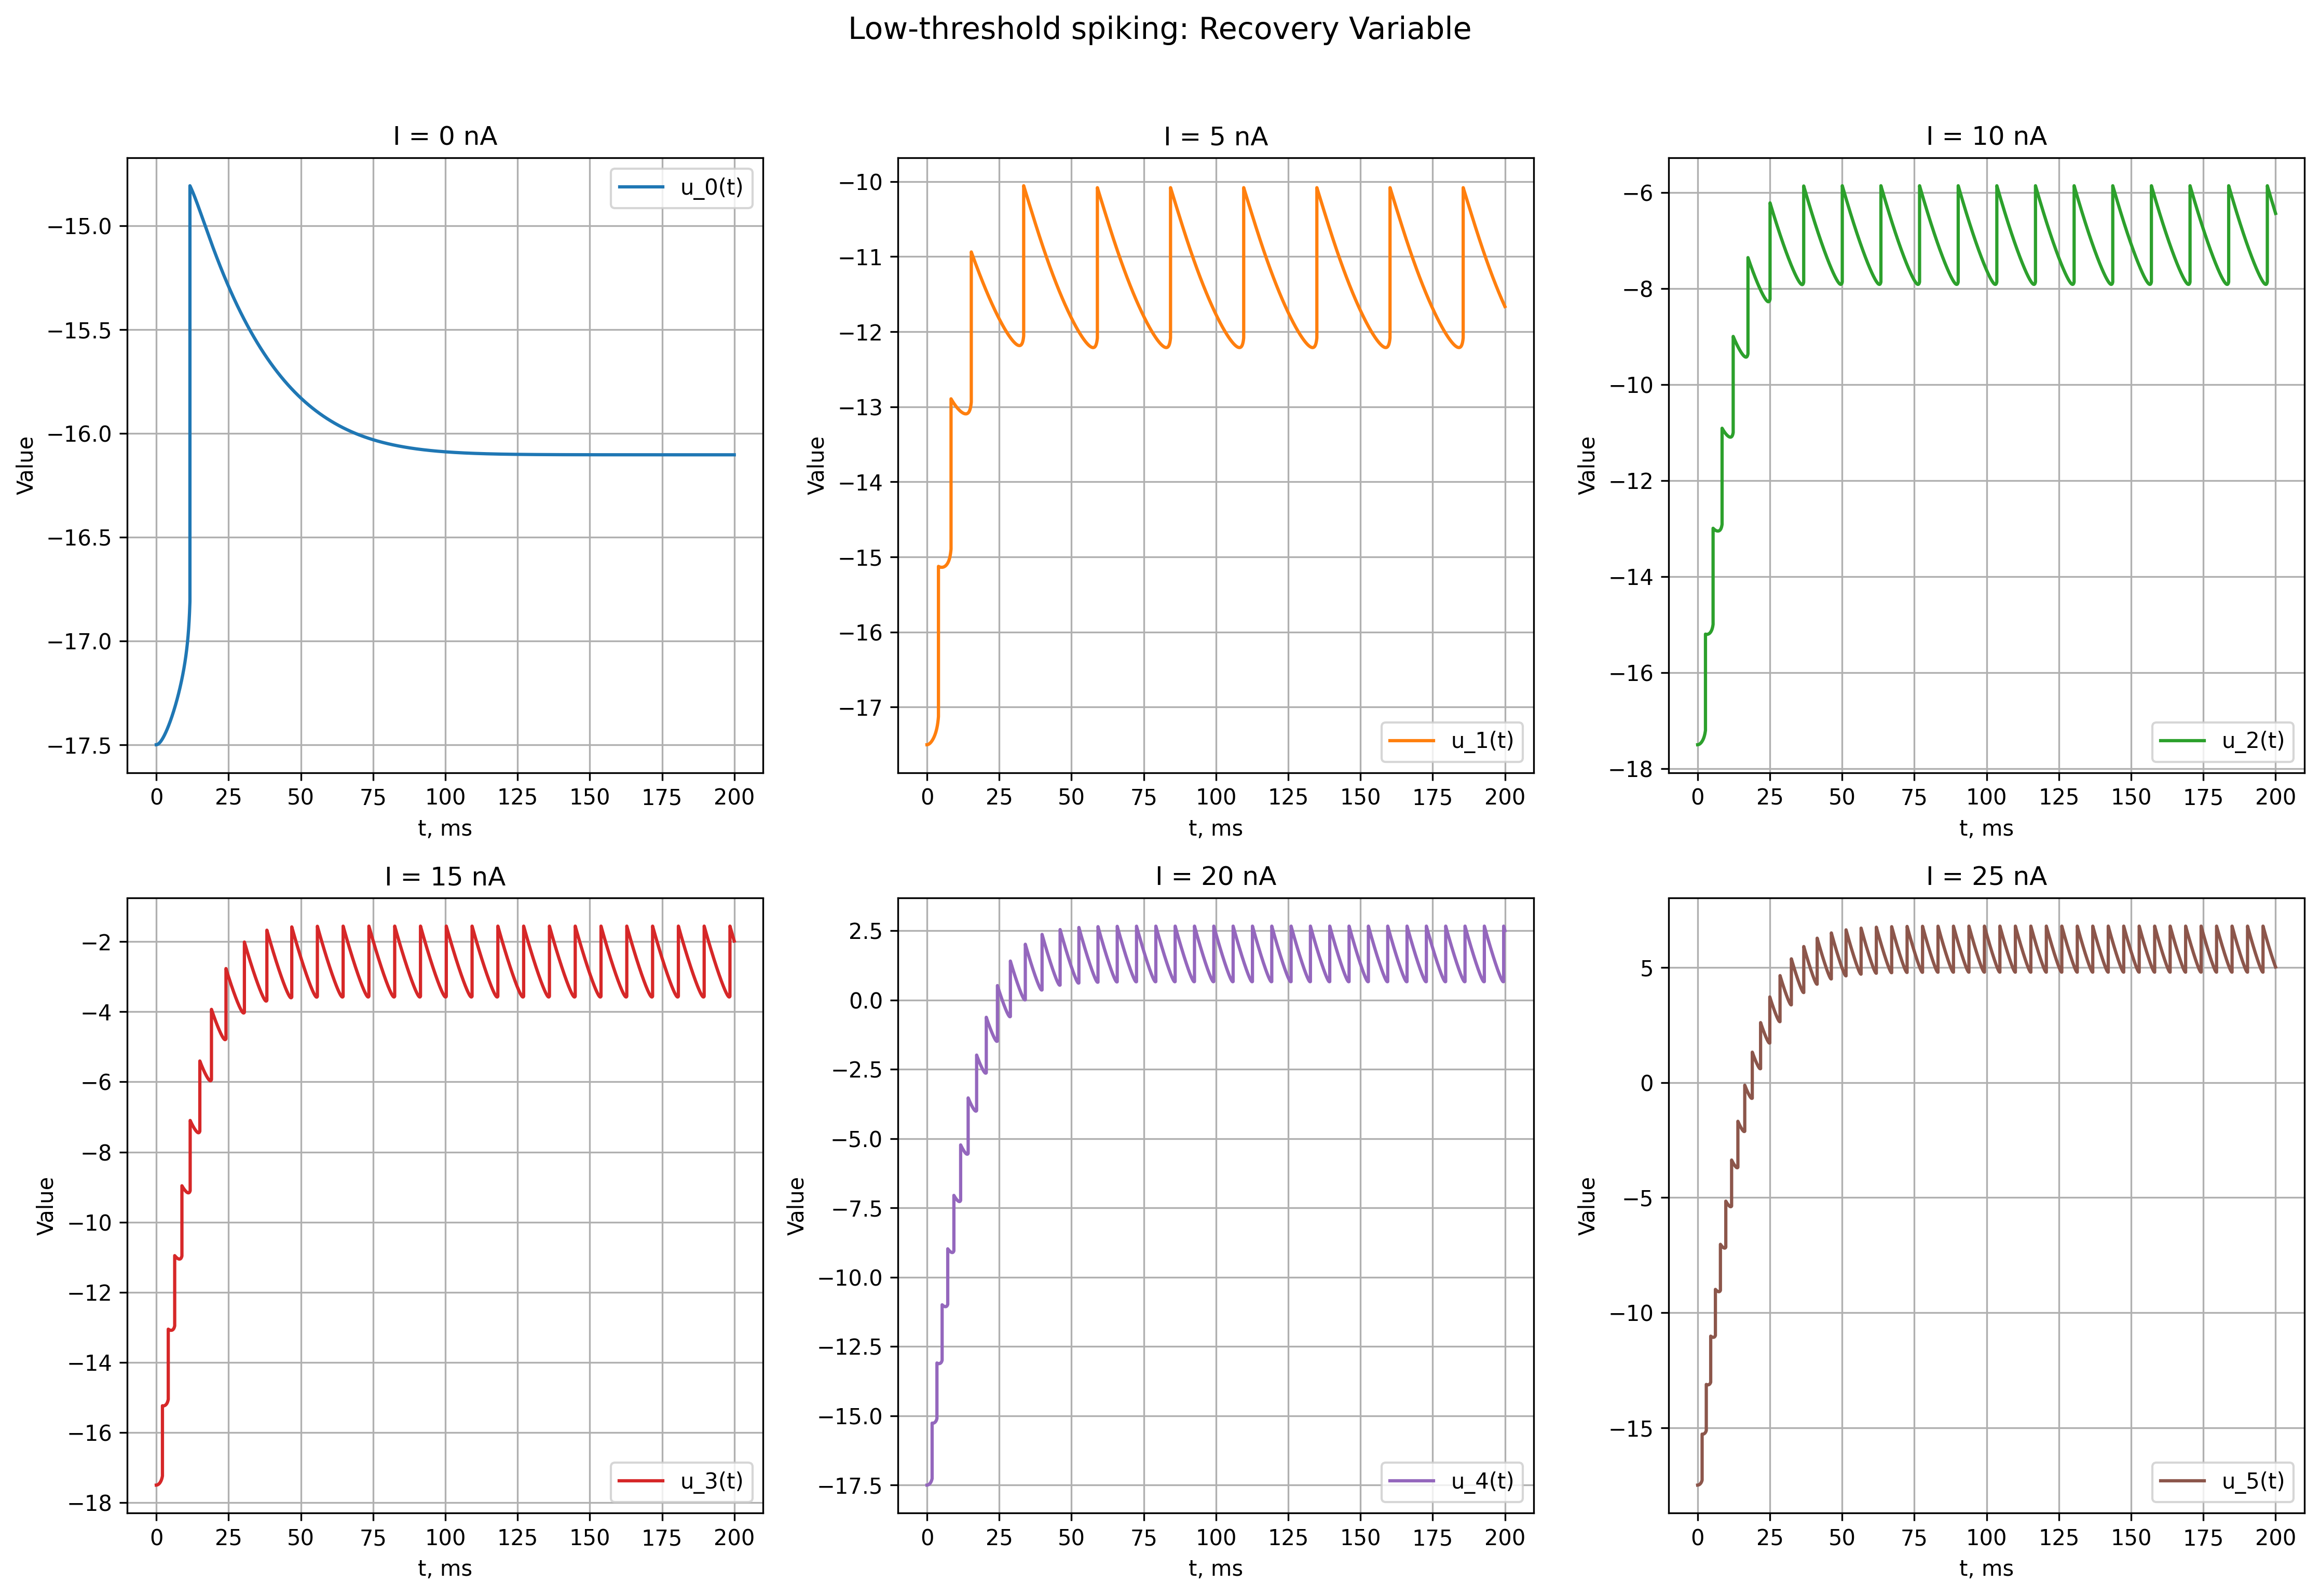
\includegraphics[width=1\linewidth]{pic/lts_different_I_recovery.png}}
	\caption{Визуализация $u(t)$ низкопорогового спайкового нейрона для разных значений $I$.}
	\label{lts_different_I_recovery}
\end{figure}

\begin{figure}[h]
\center{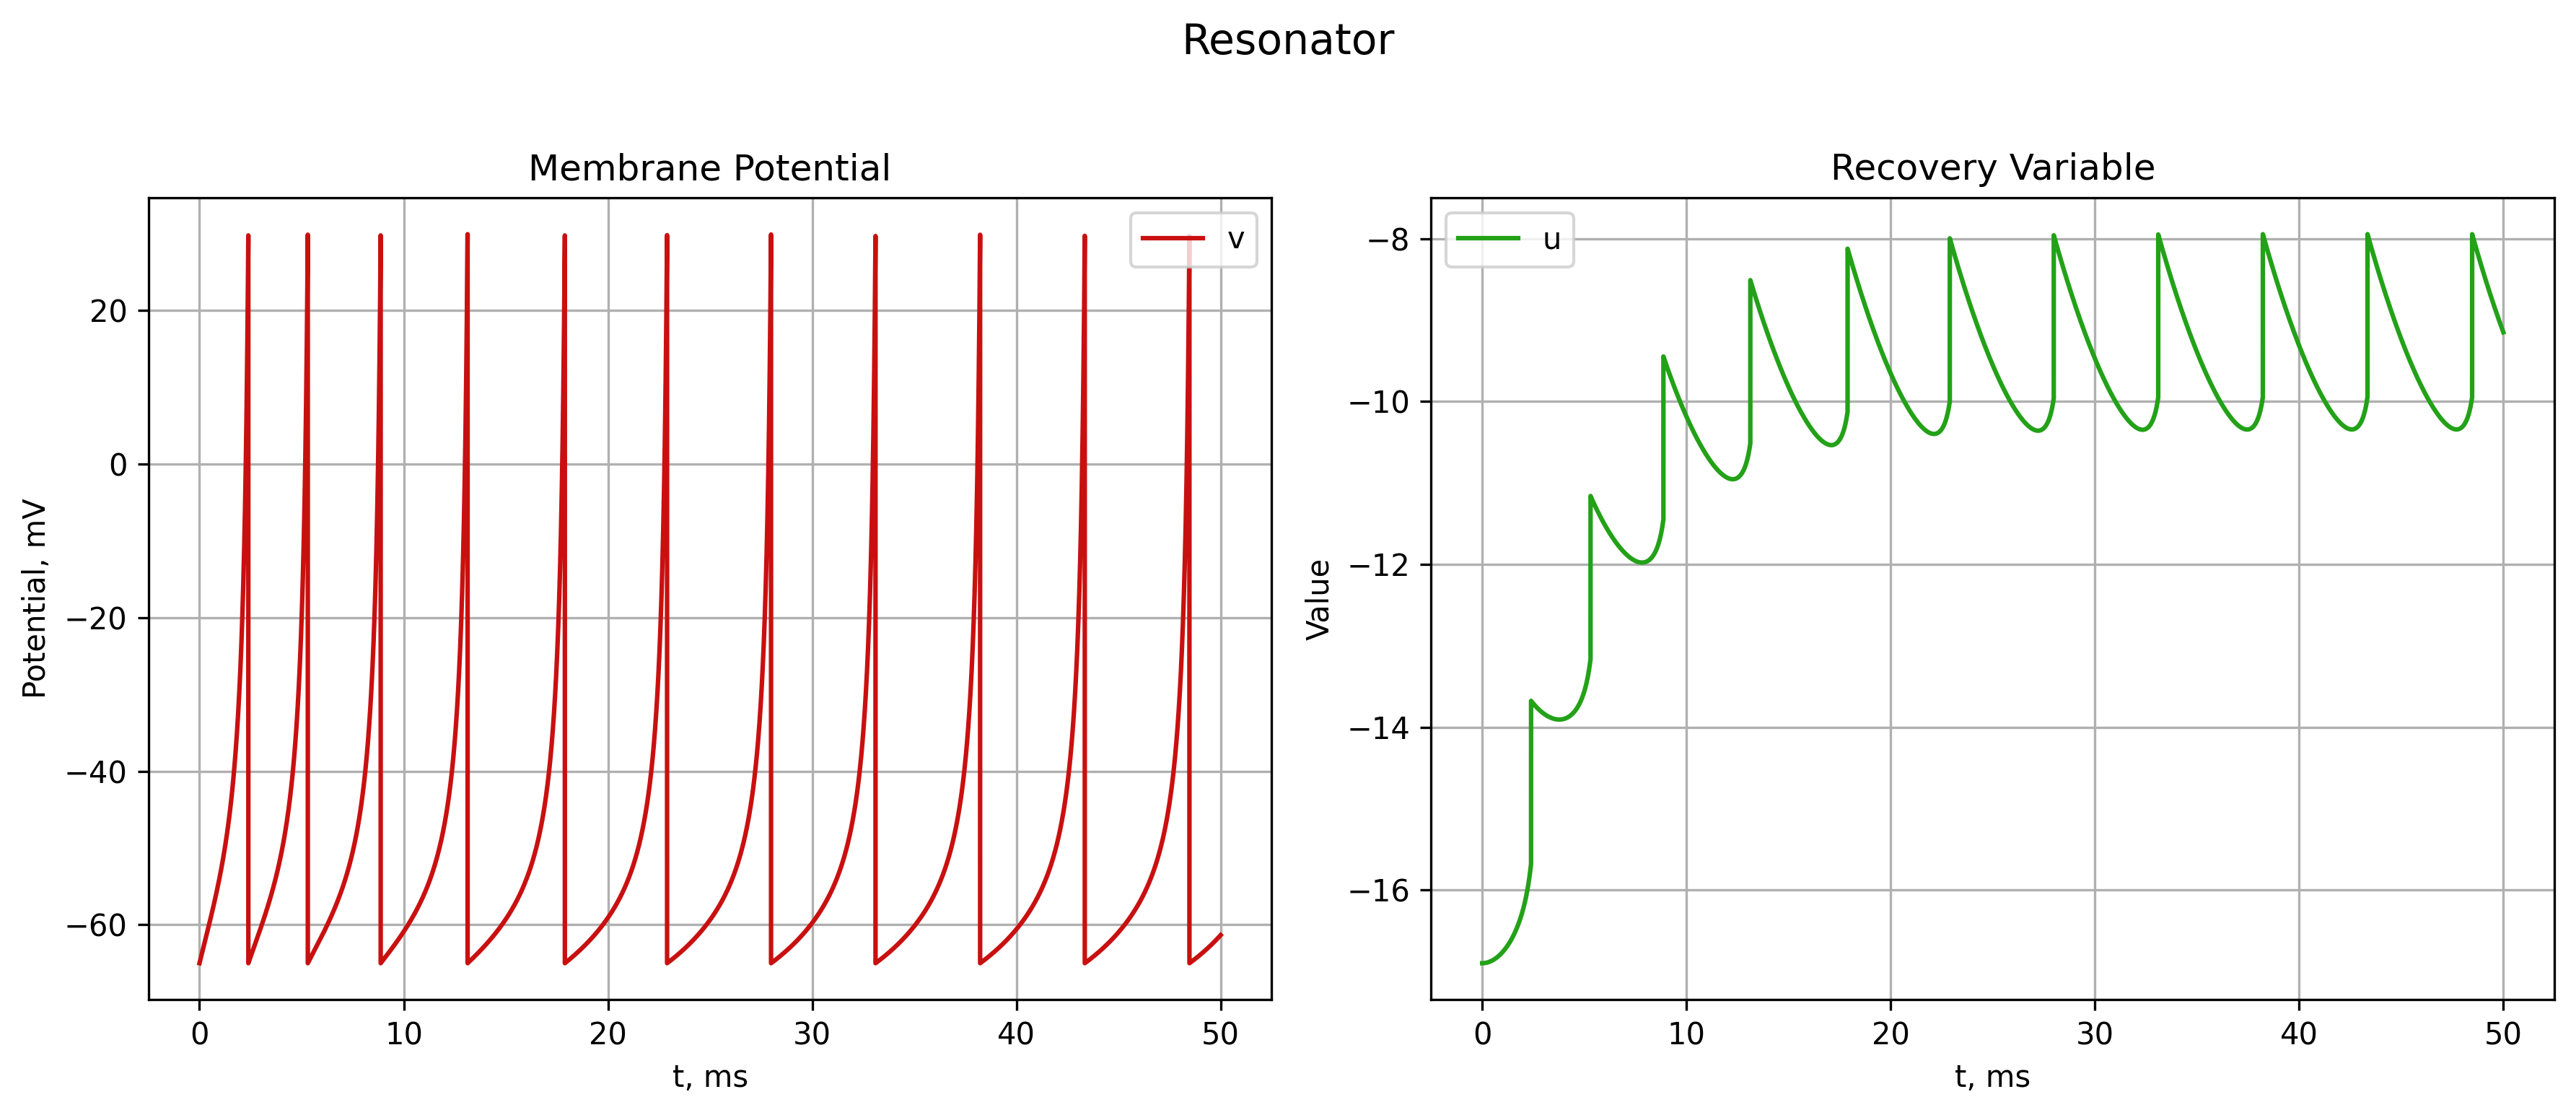
\includegraphics[width=1\linewidth]{pic/resonator_spiking.png}}
\caption{Визуализация резиллерно-спайкового нейрона при $I=10$ нА.}
\label{1_rz}
\end{figure}

\begin{figure}[h]
	\center{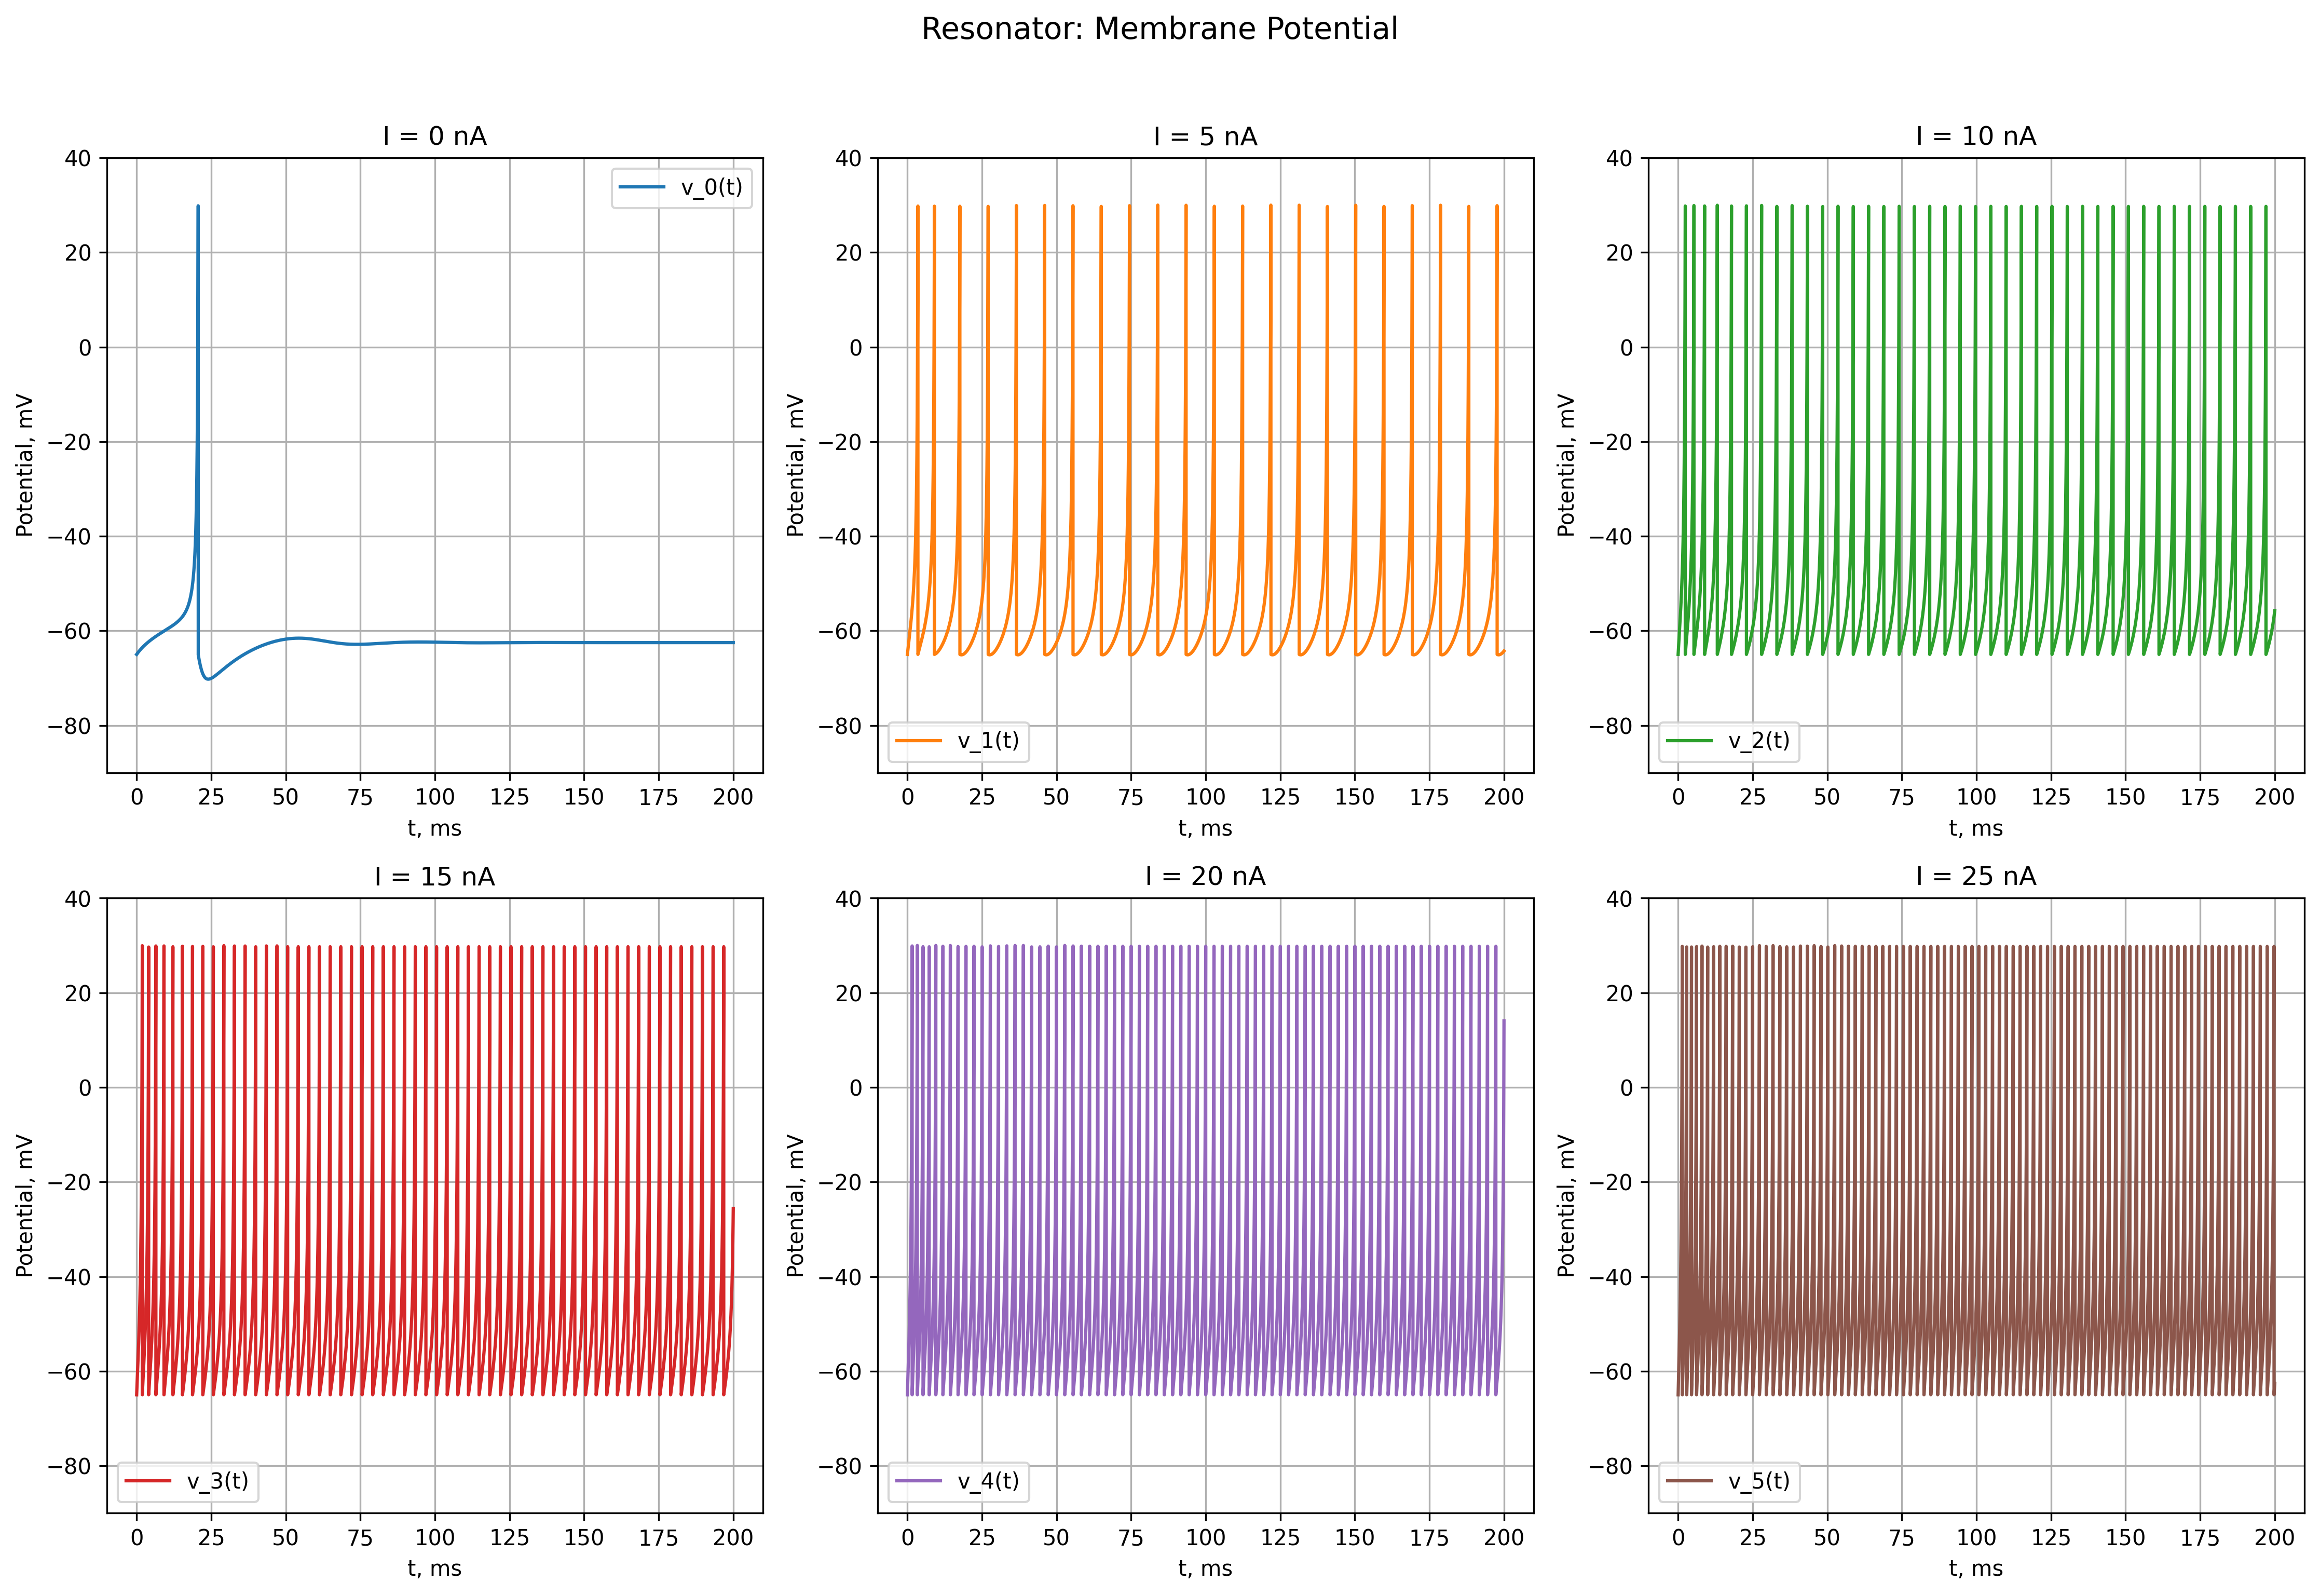
\includegraphics[width=1\linewidth]{pic/rz_different_I_potentials.png}}
	\caption{Визуализация $v(t)$ резиллерно-спайкового нейрона для разных значений $I$.}
	\label{rz_different_I_potentials}
\end{figure}

\begin{figure}[h]
	\center{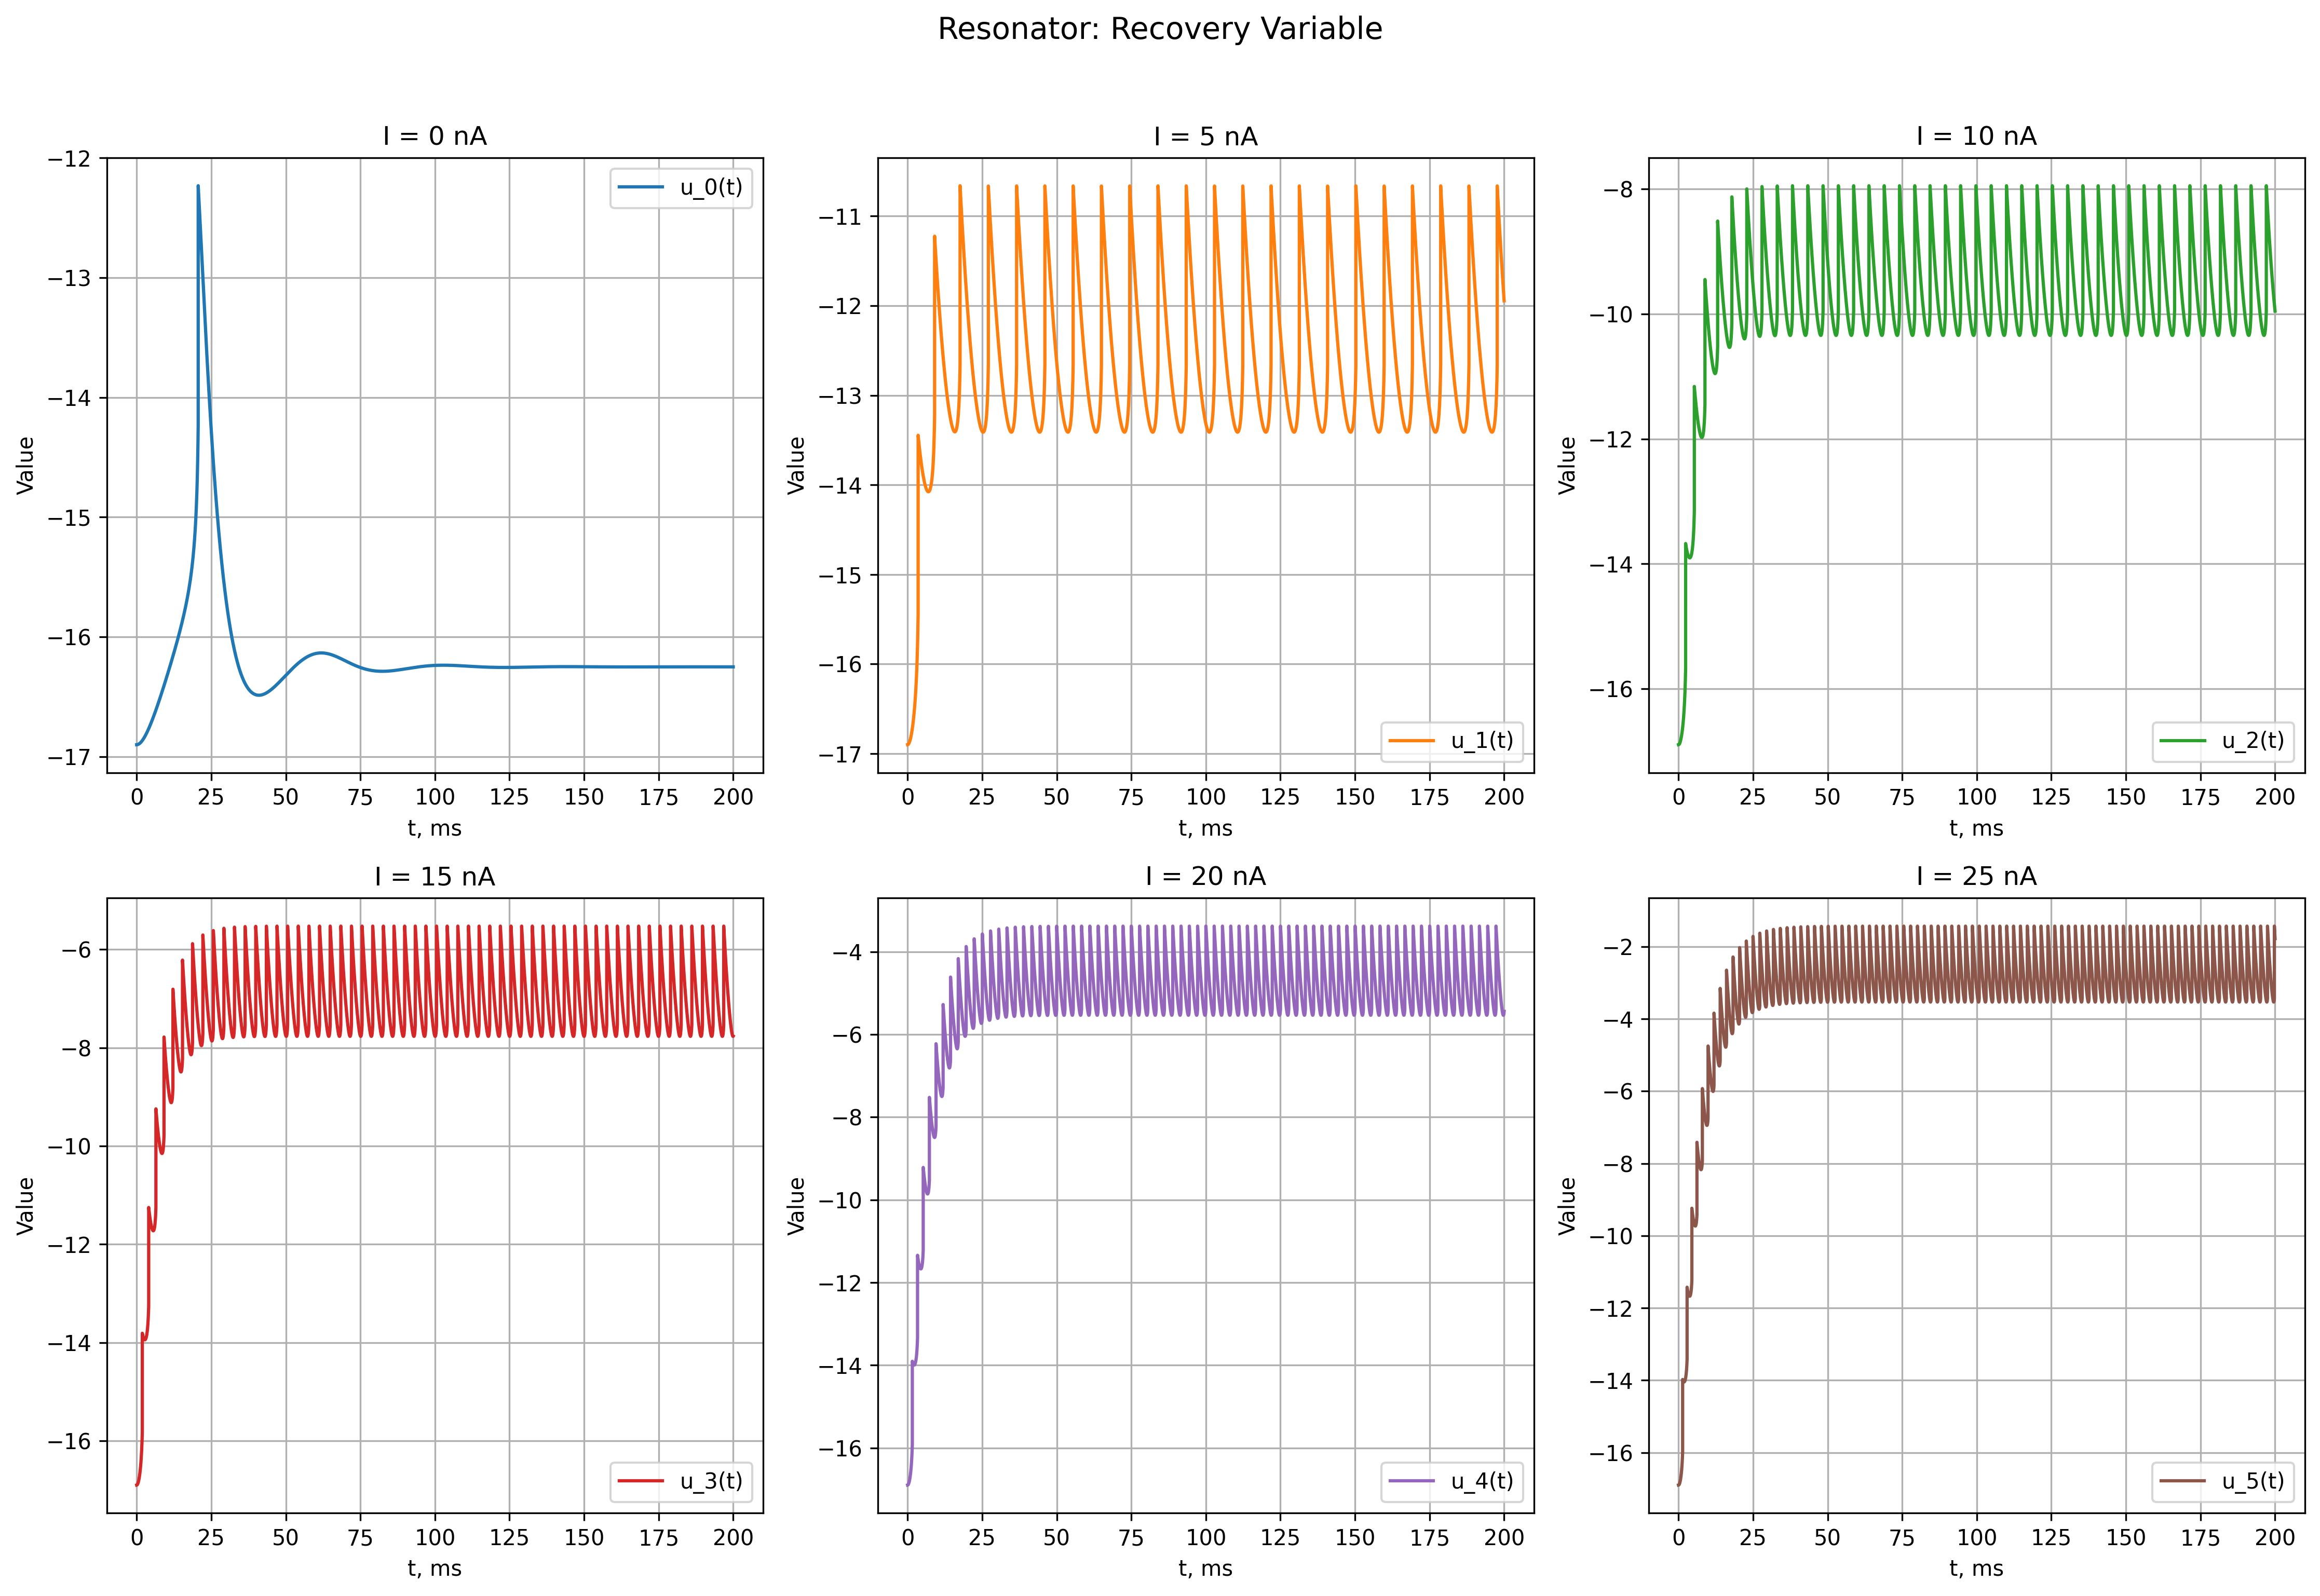
\includegraphics[width=1\linewidth]{pic/rz_different_I_recovery.png}}
	\caption{Визуализация $u(t)$ резиллерно-спайкового нейрона для разных значений $I$.}
	\label{rz_different_I_recovery}
\end{figure}

\begin{figure}[h]
\center{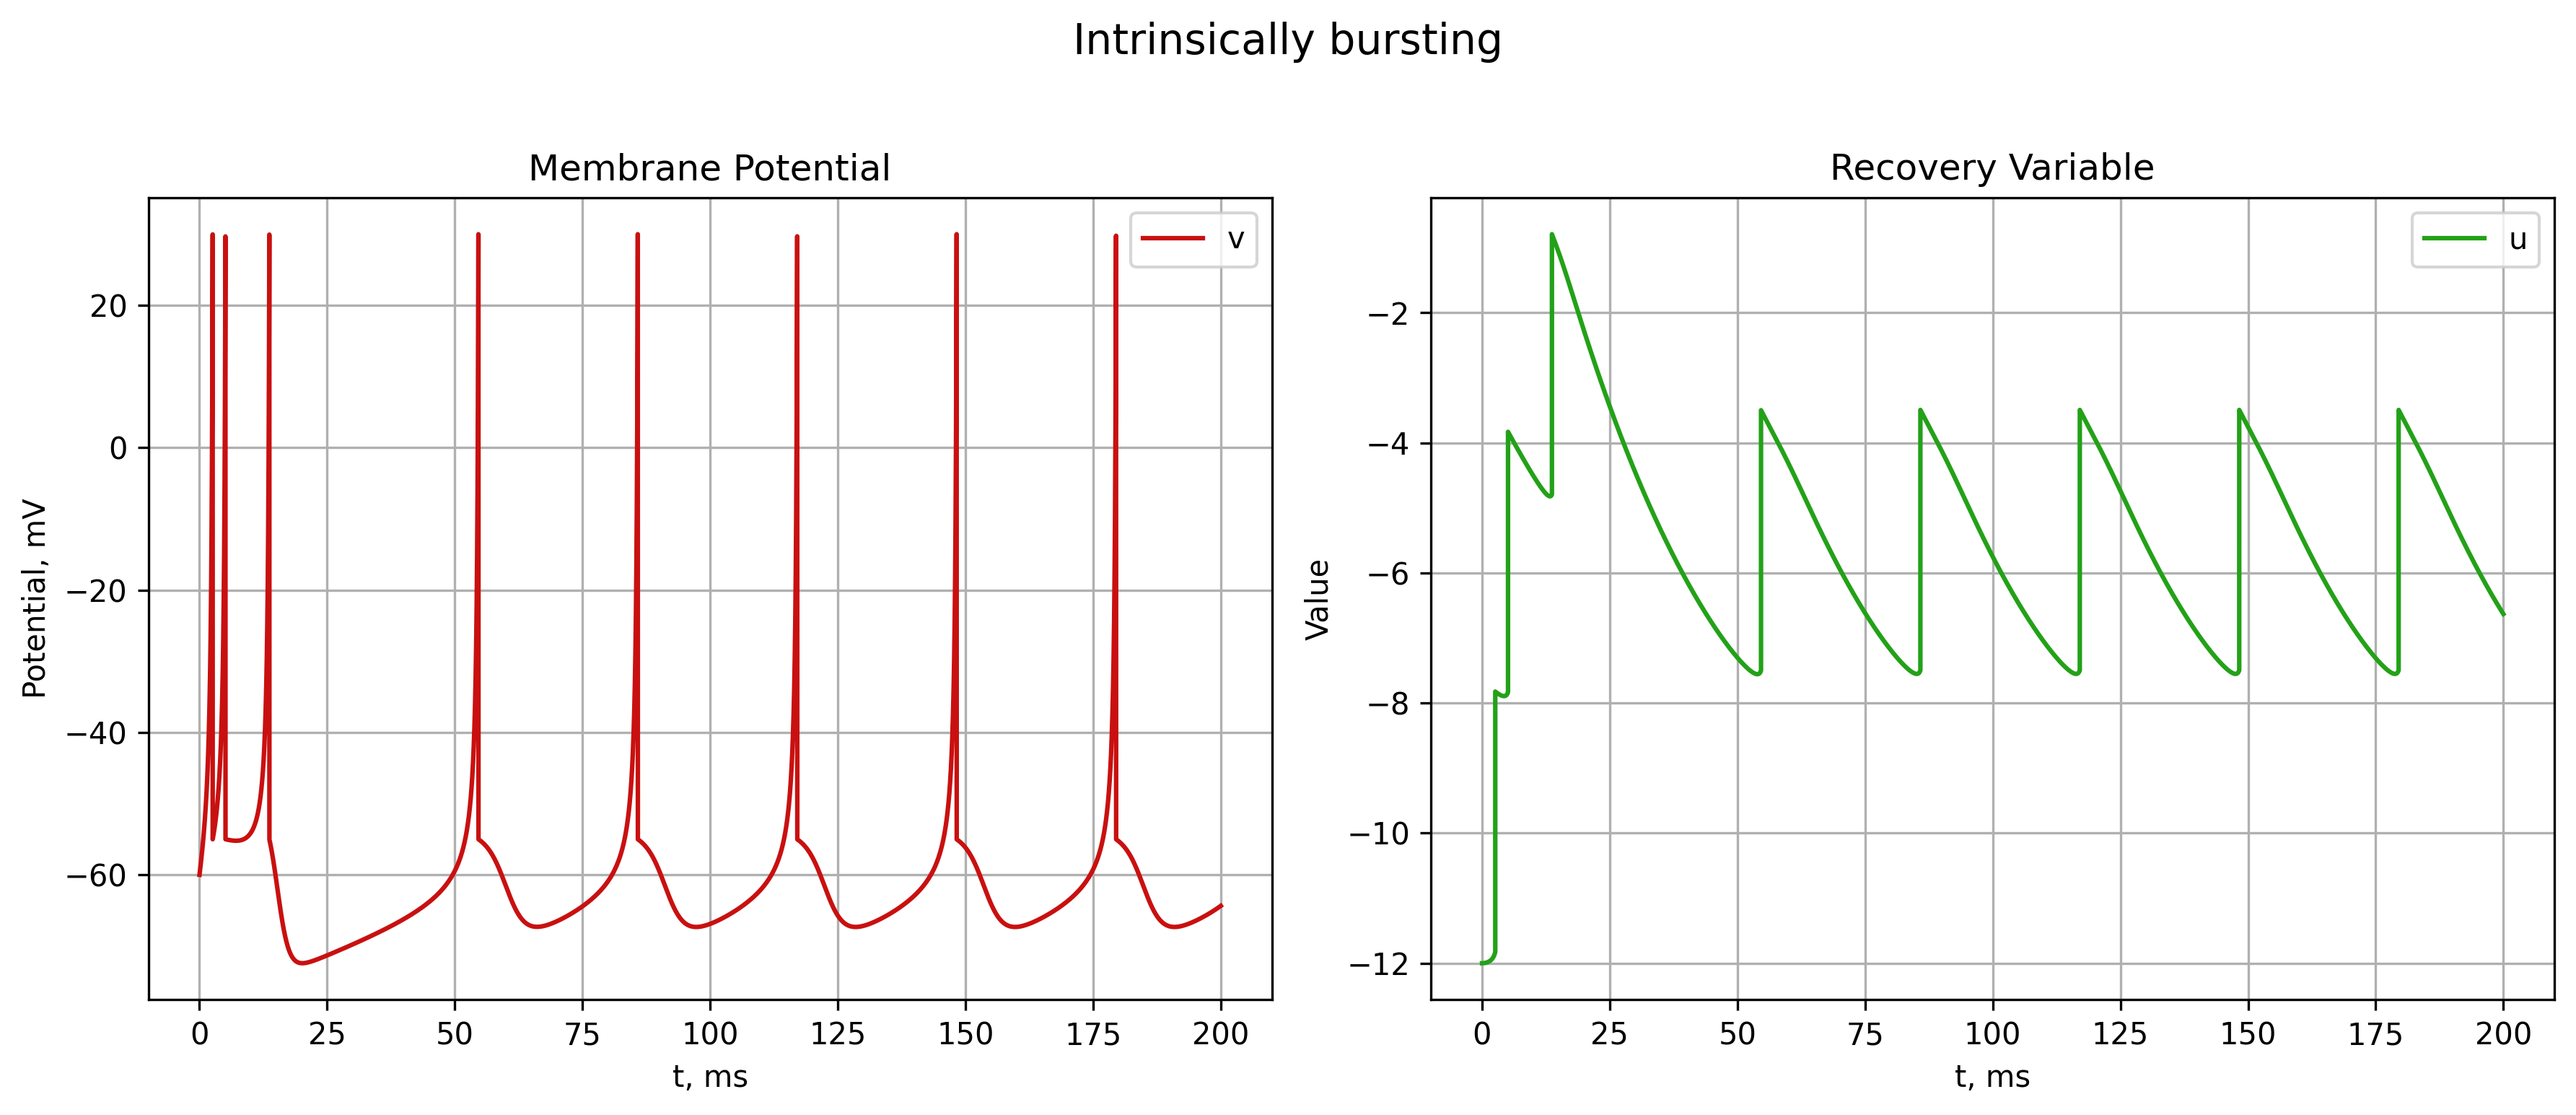
\includegraphics[width=1\linewidth]{pic/intrinsically_bursting.png}}
\caption{Визуализация интринсивно-всплескового нейрона при $I=10$ нА.}
\label{1_ib}
\end{figure}

\begin{figure}[h]
	\center{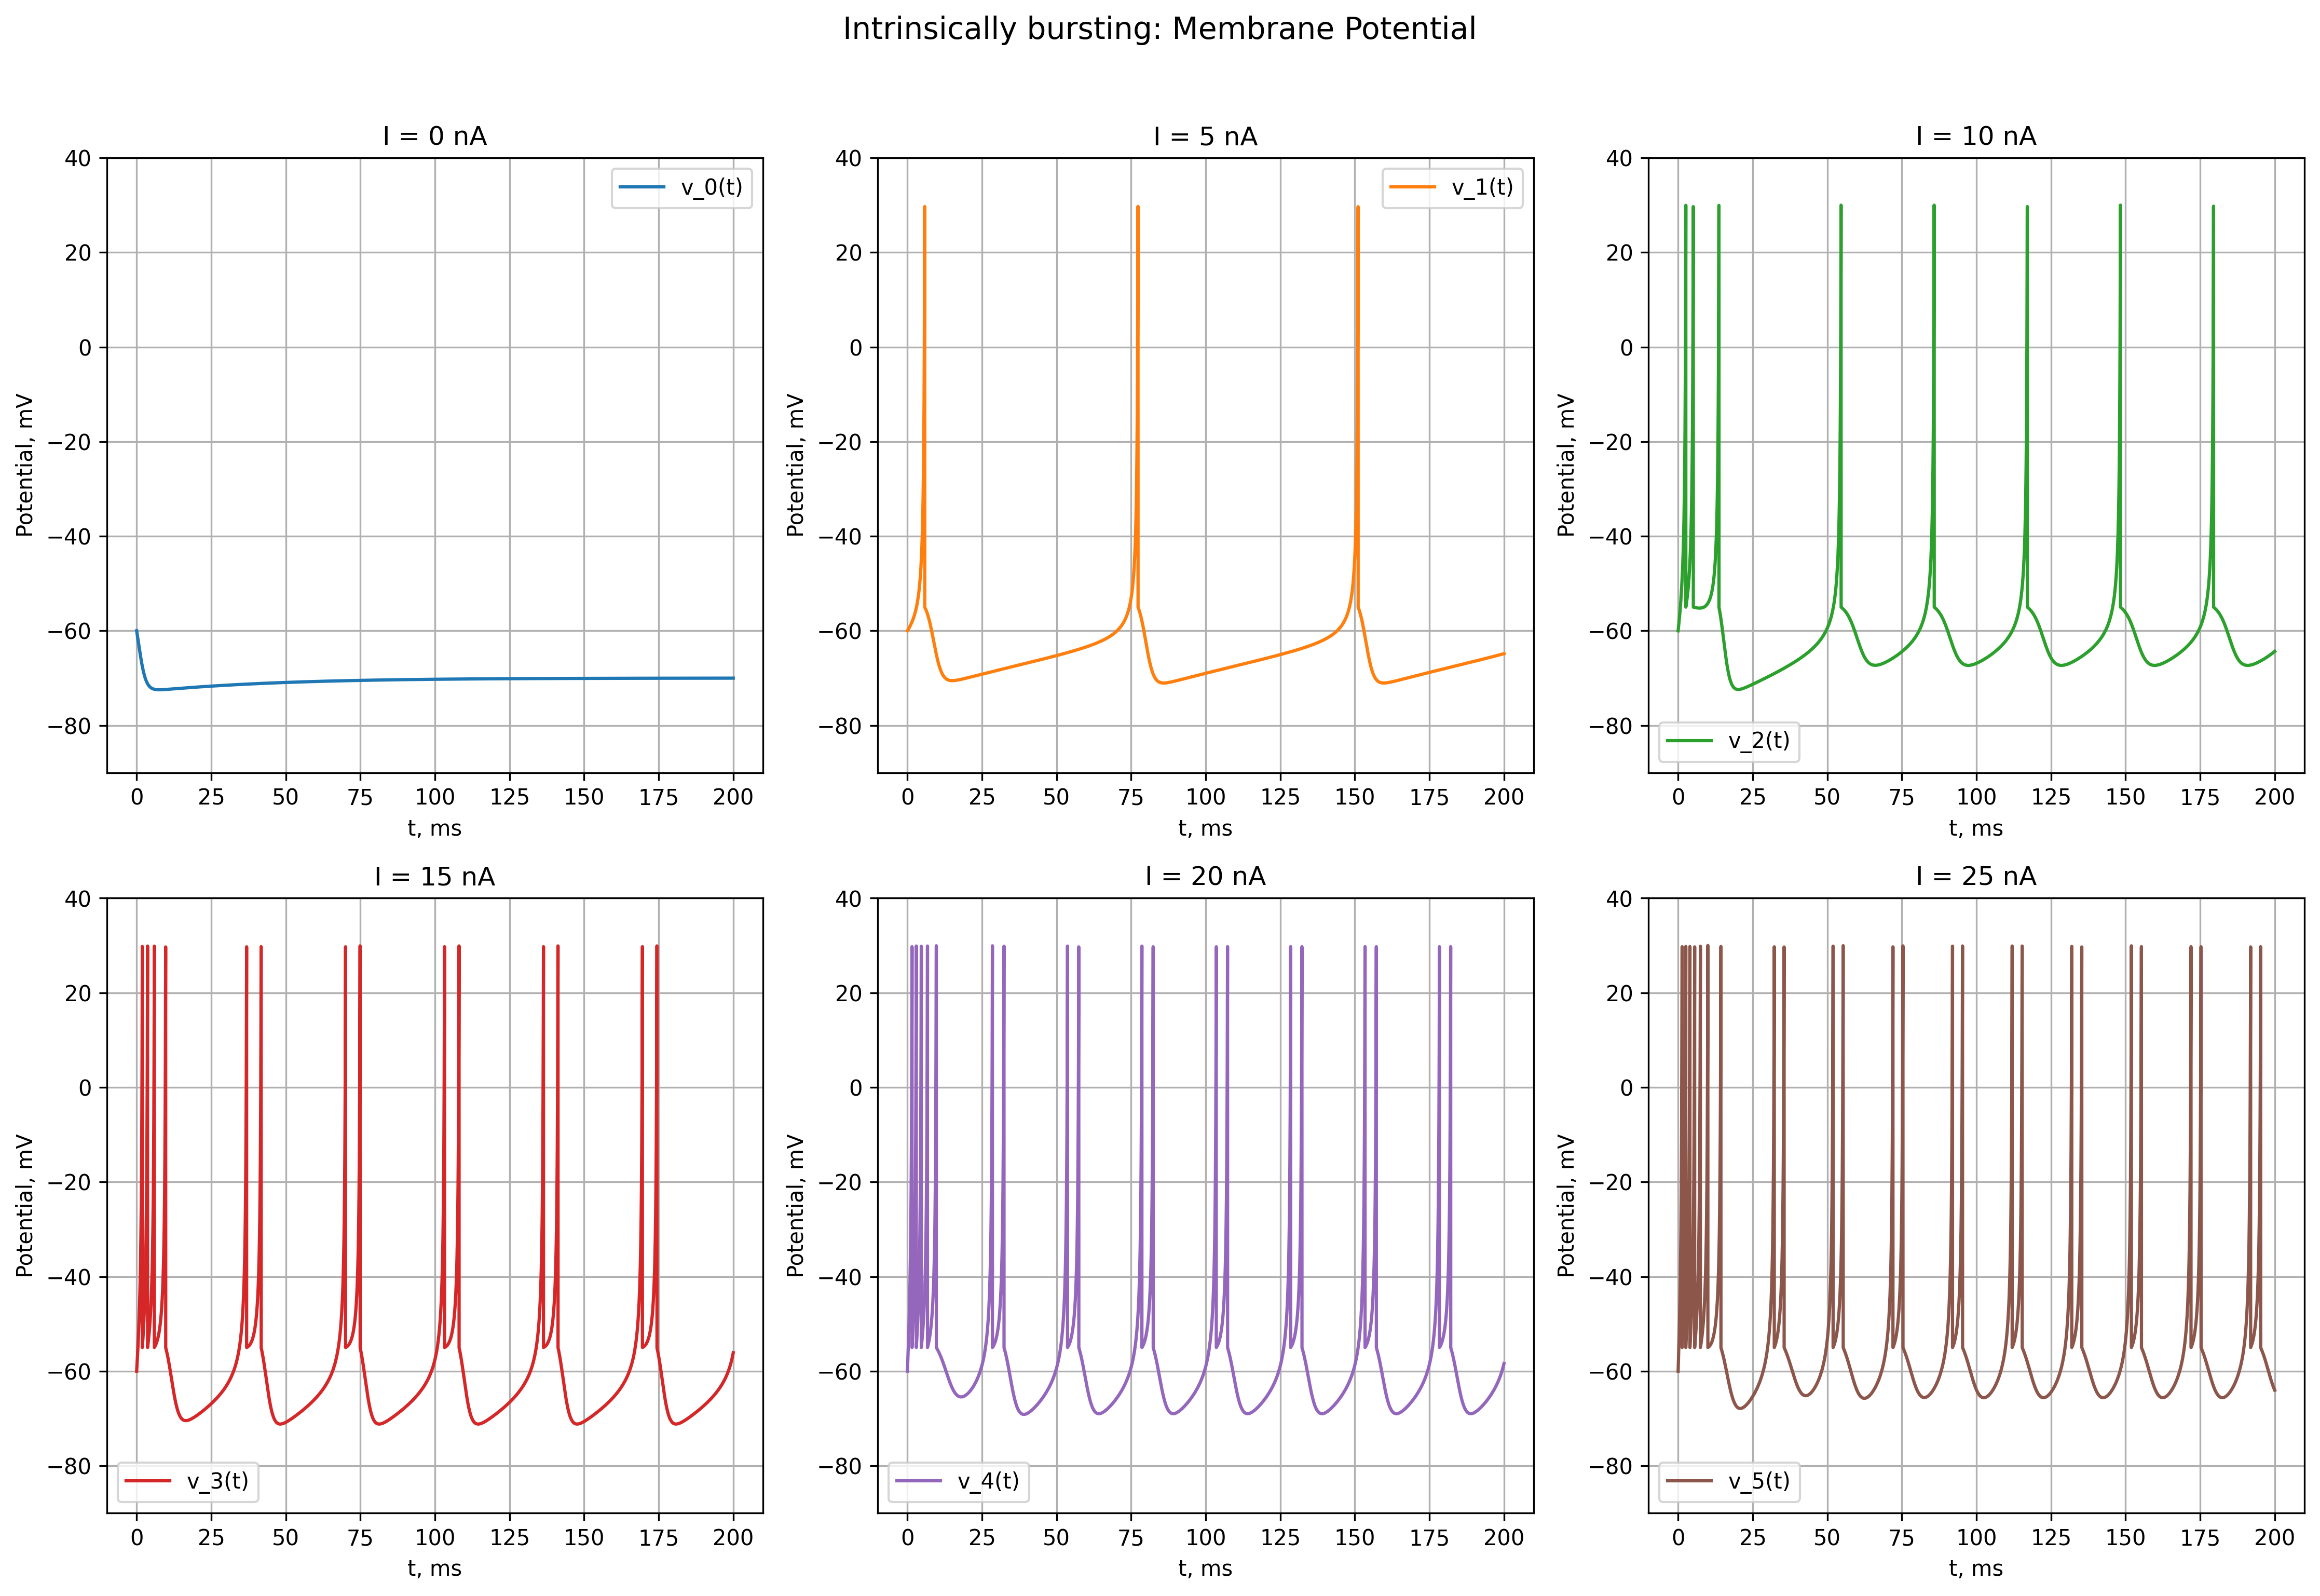
\includegraphics[width=1\linewidth]{pic/ib_different_I_potentials.png}}
	\caption{Визуализация $v(t)$ интринсивно-всплескового нейрона для разных значений $I$.}
	\label{ib_different_I_potentials}
\end{figure}

\begin{figure}[h]
	\center{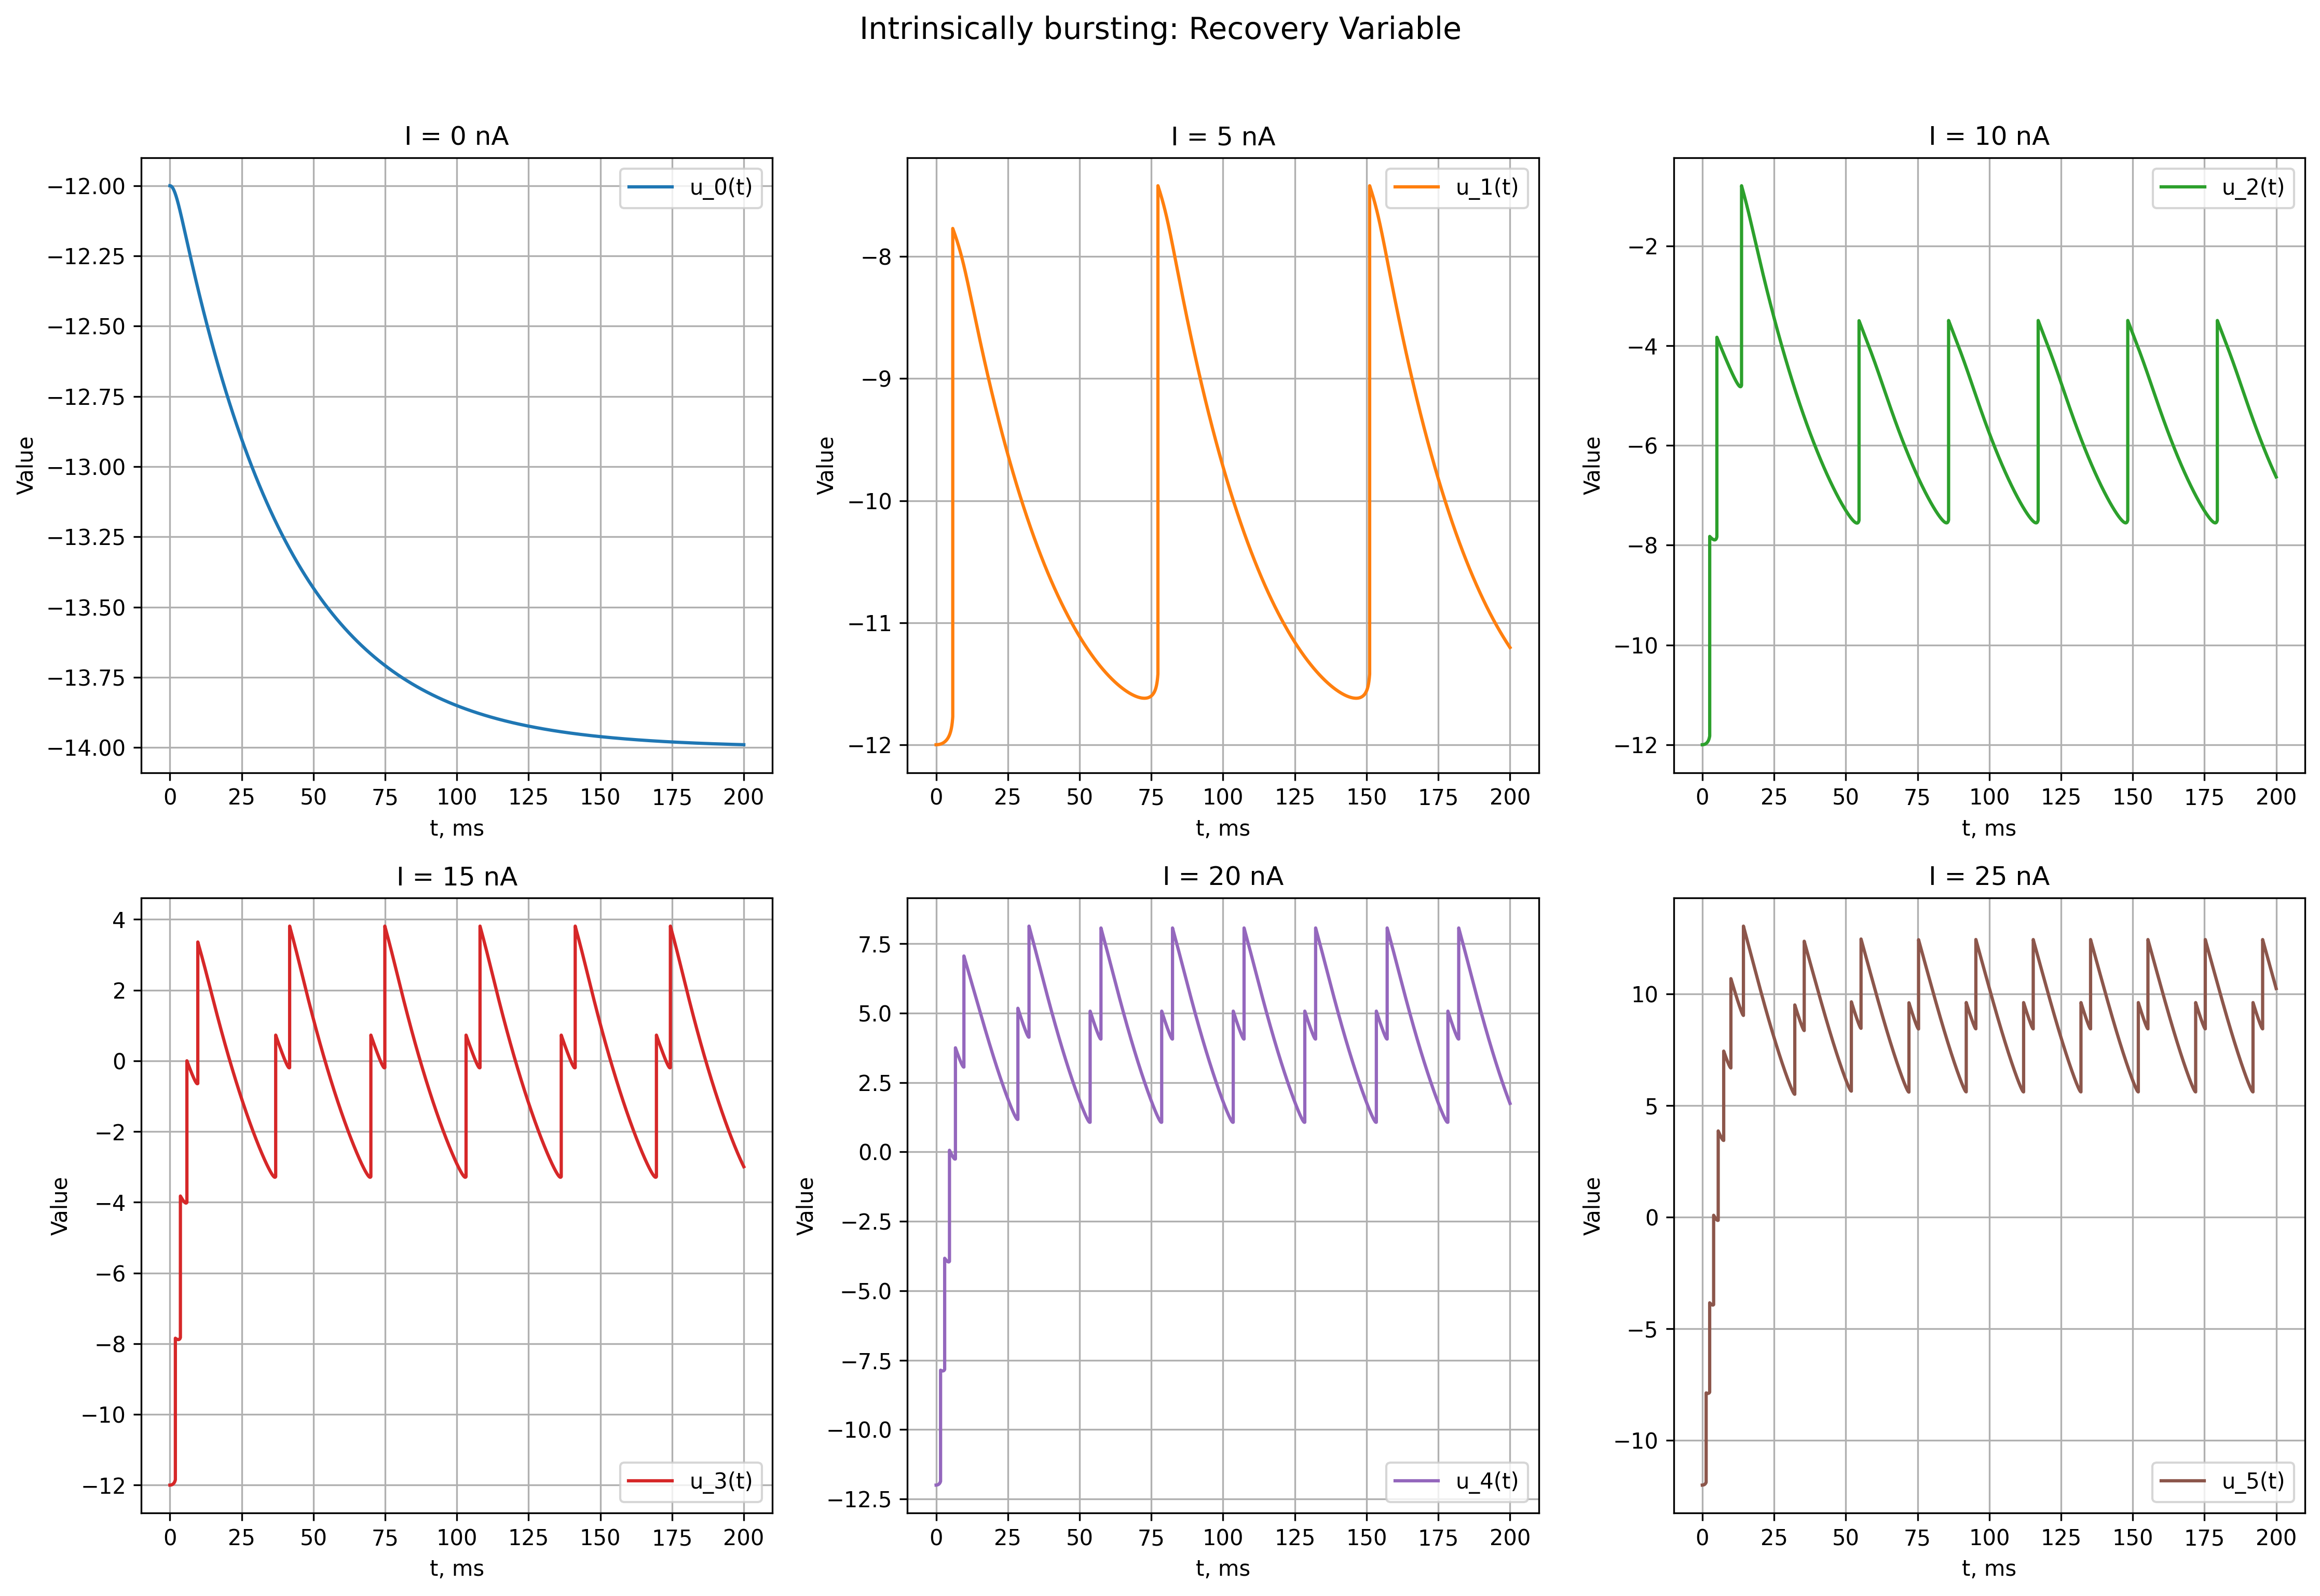
\includegraphics[width=1\linewidth]{pic/ib_different_I_recovery.png}}
	\caption{Визуализация $u(t)$ интринсивно-всплескового нейрона для разных значений $I$.}
	\label{ib_different_I_recovery}
\end{figure}

\begin{figure}[h]
\center{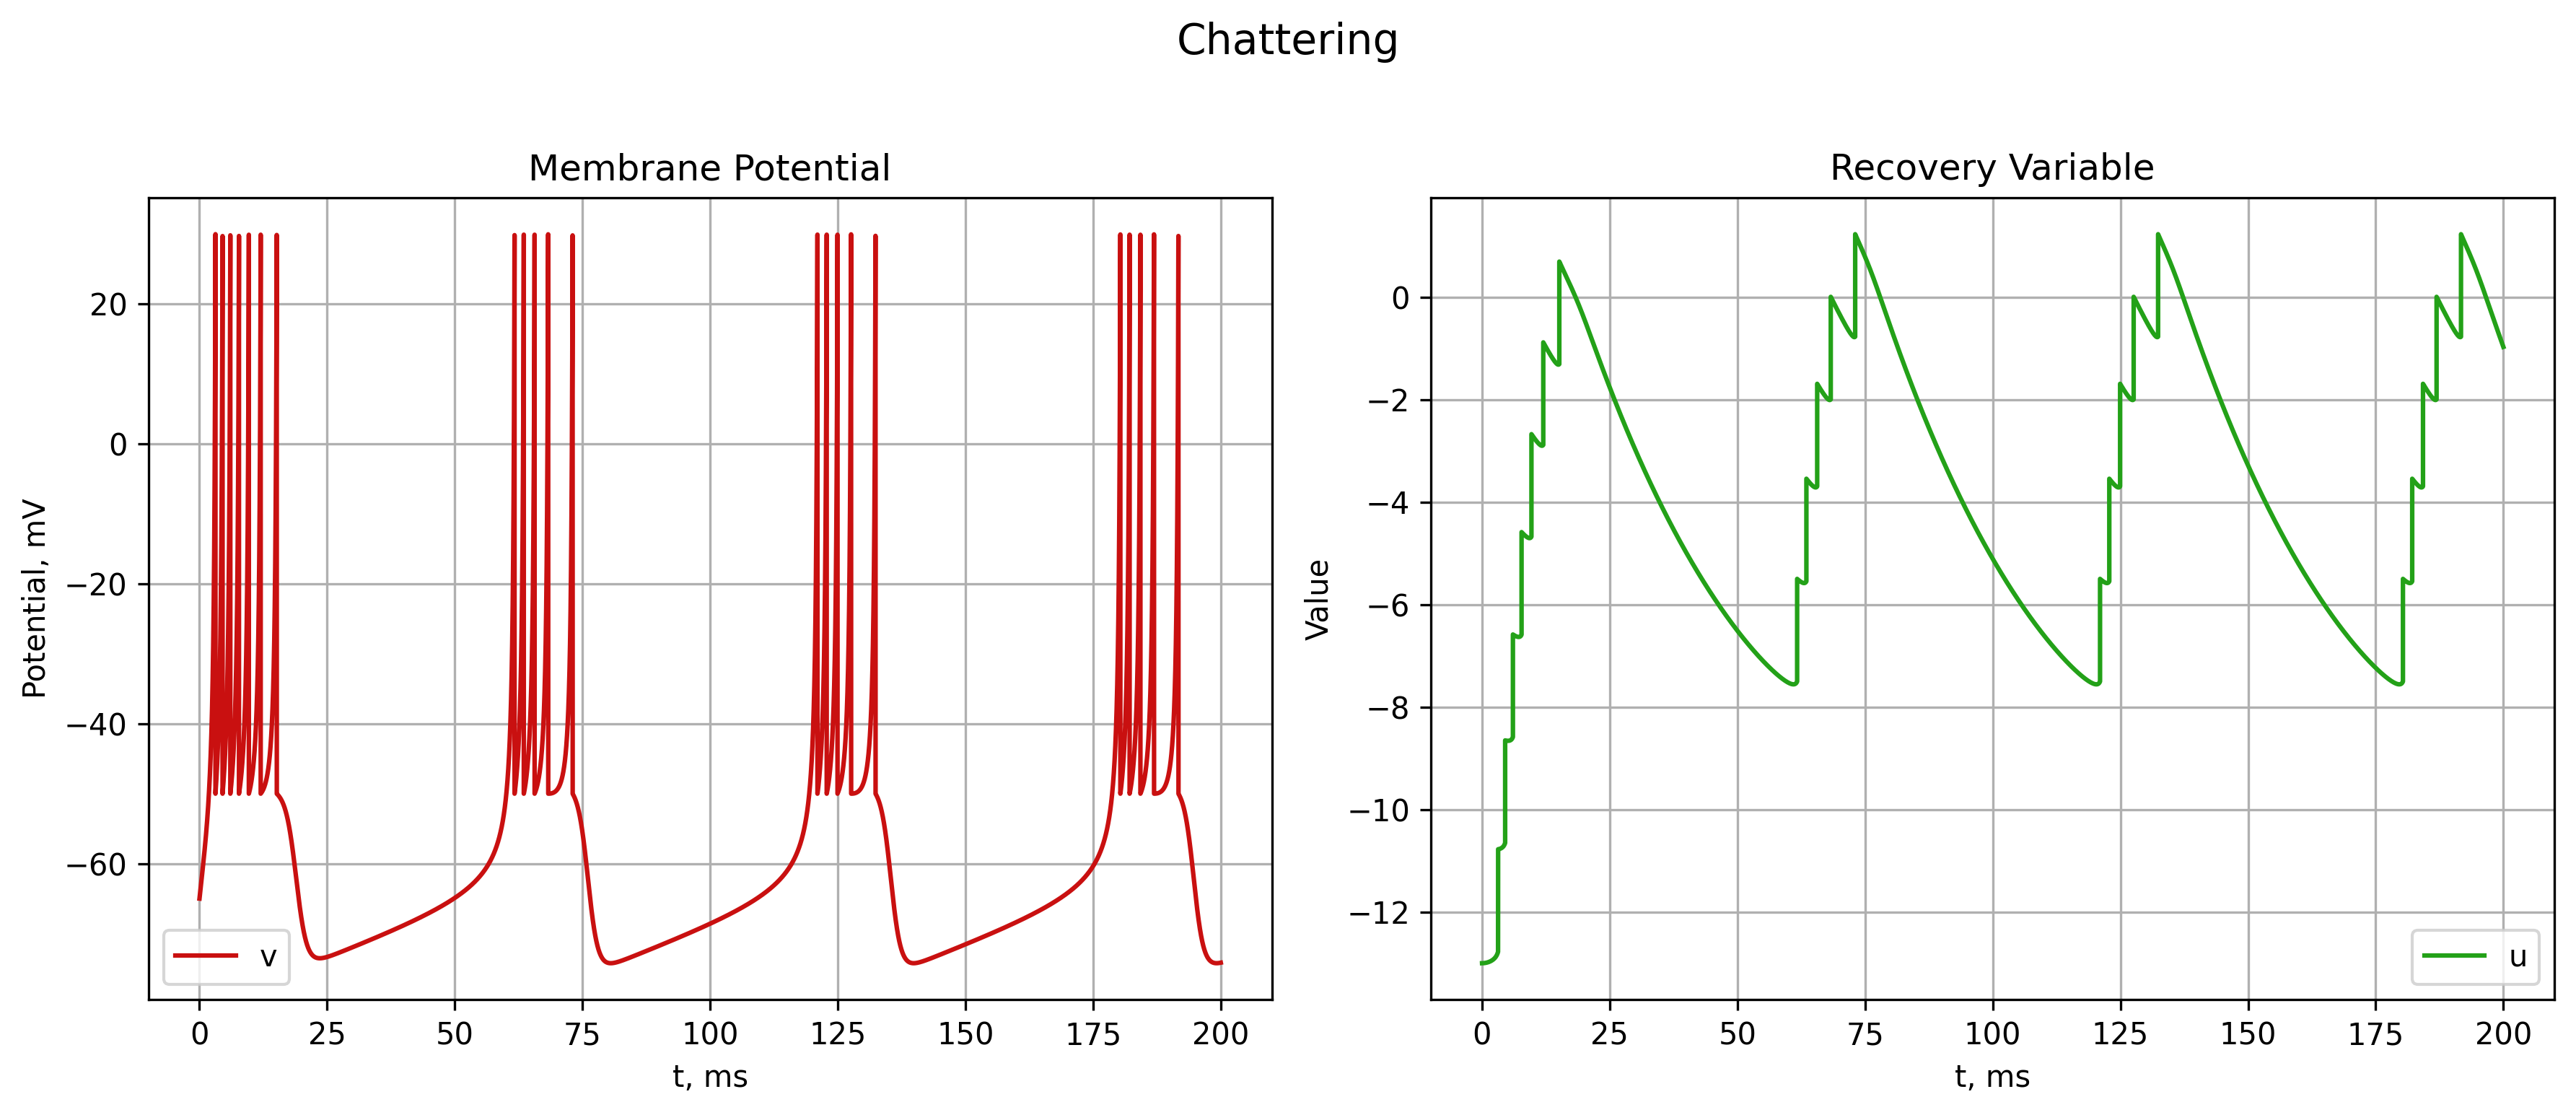
\includegraphics[width=1\linewidth]{pic/chattering.png}}
\caption{Визуализация частотного нейрона при $I=10$ нА.}
\label{1_ch}
\end{figure}

\begin{figure}[h]
	\center{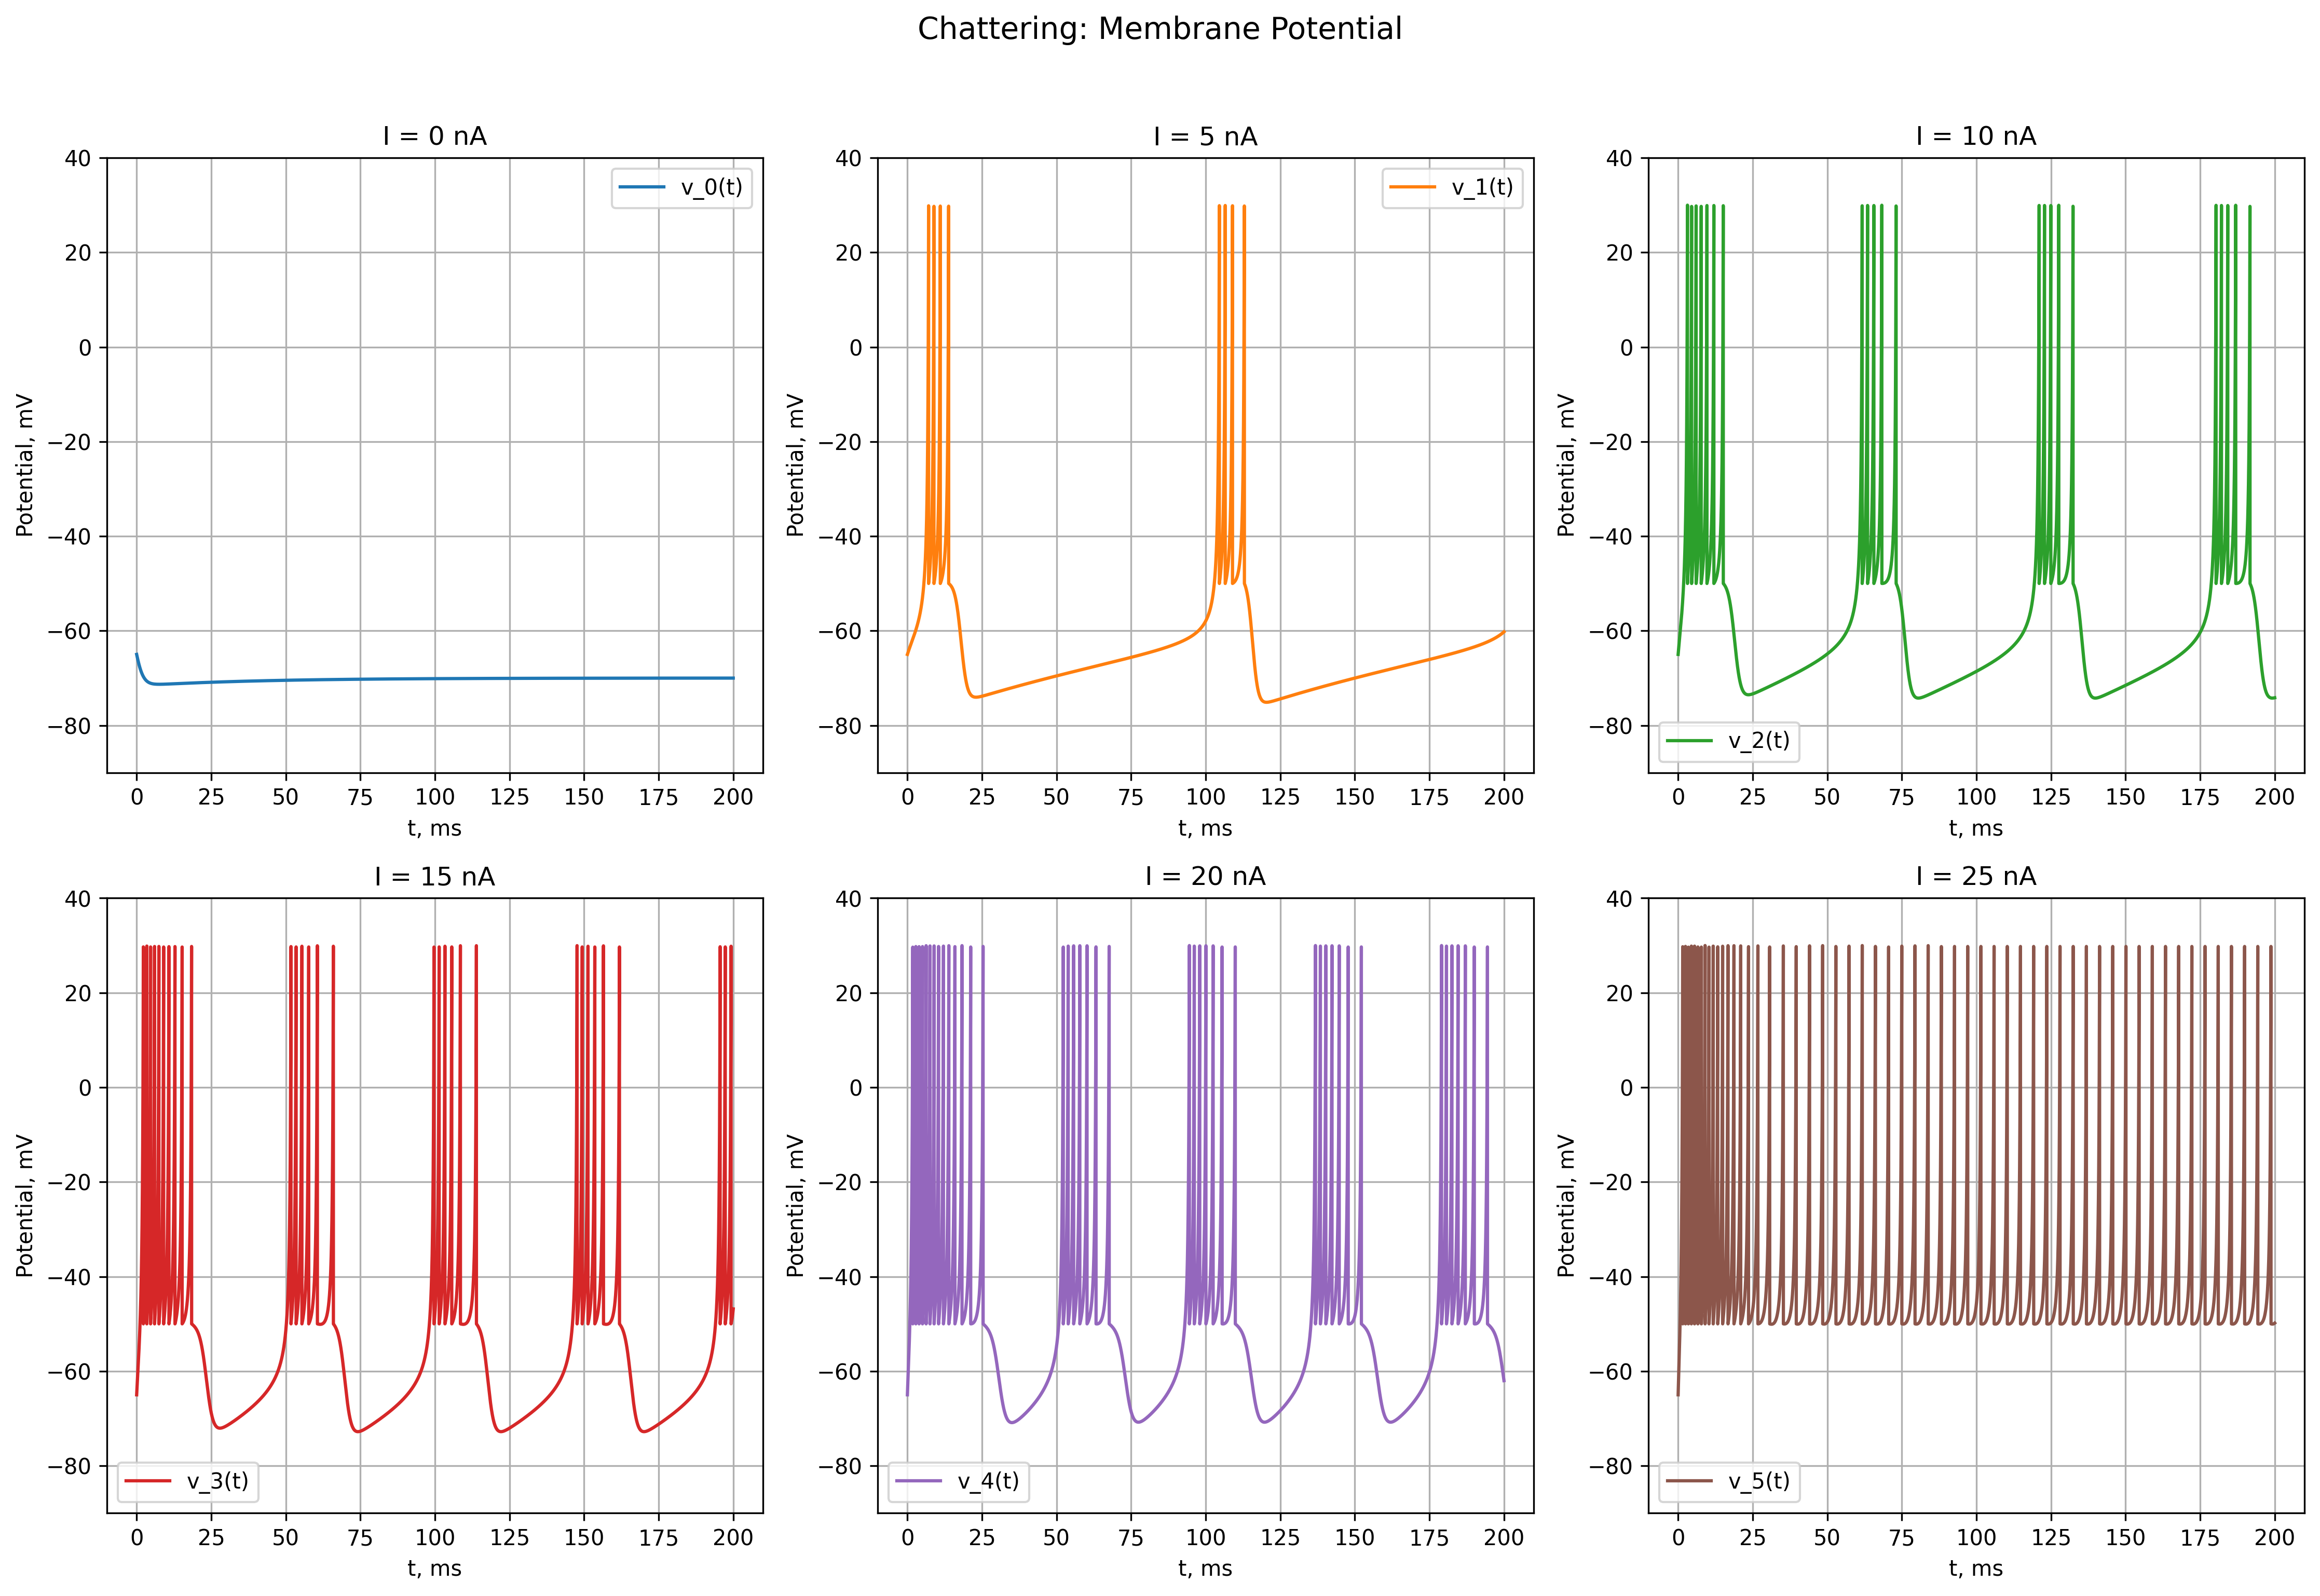
\includegraphics[width=1\linewidth]{pic/ch_different_I_potentials.png}}
	\caption{Визуализация $v(t)$ частотного нейрона для разных значений $I$.}
	\label{ch_different_I_potentials}
\end{figure}

\begin{figure}[h]
	\center{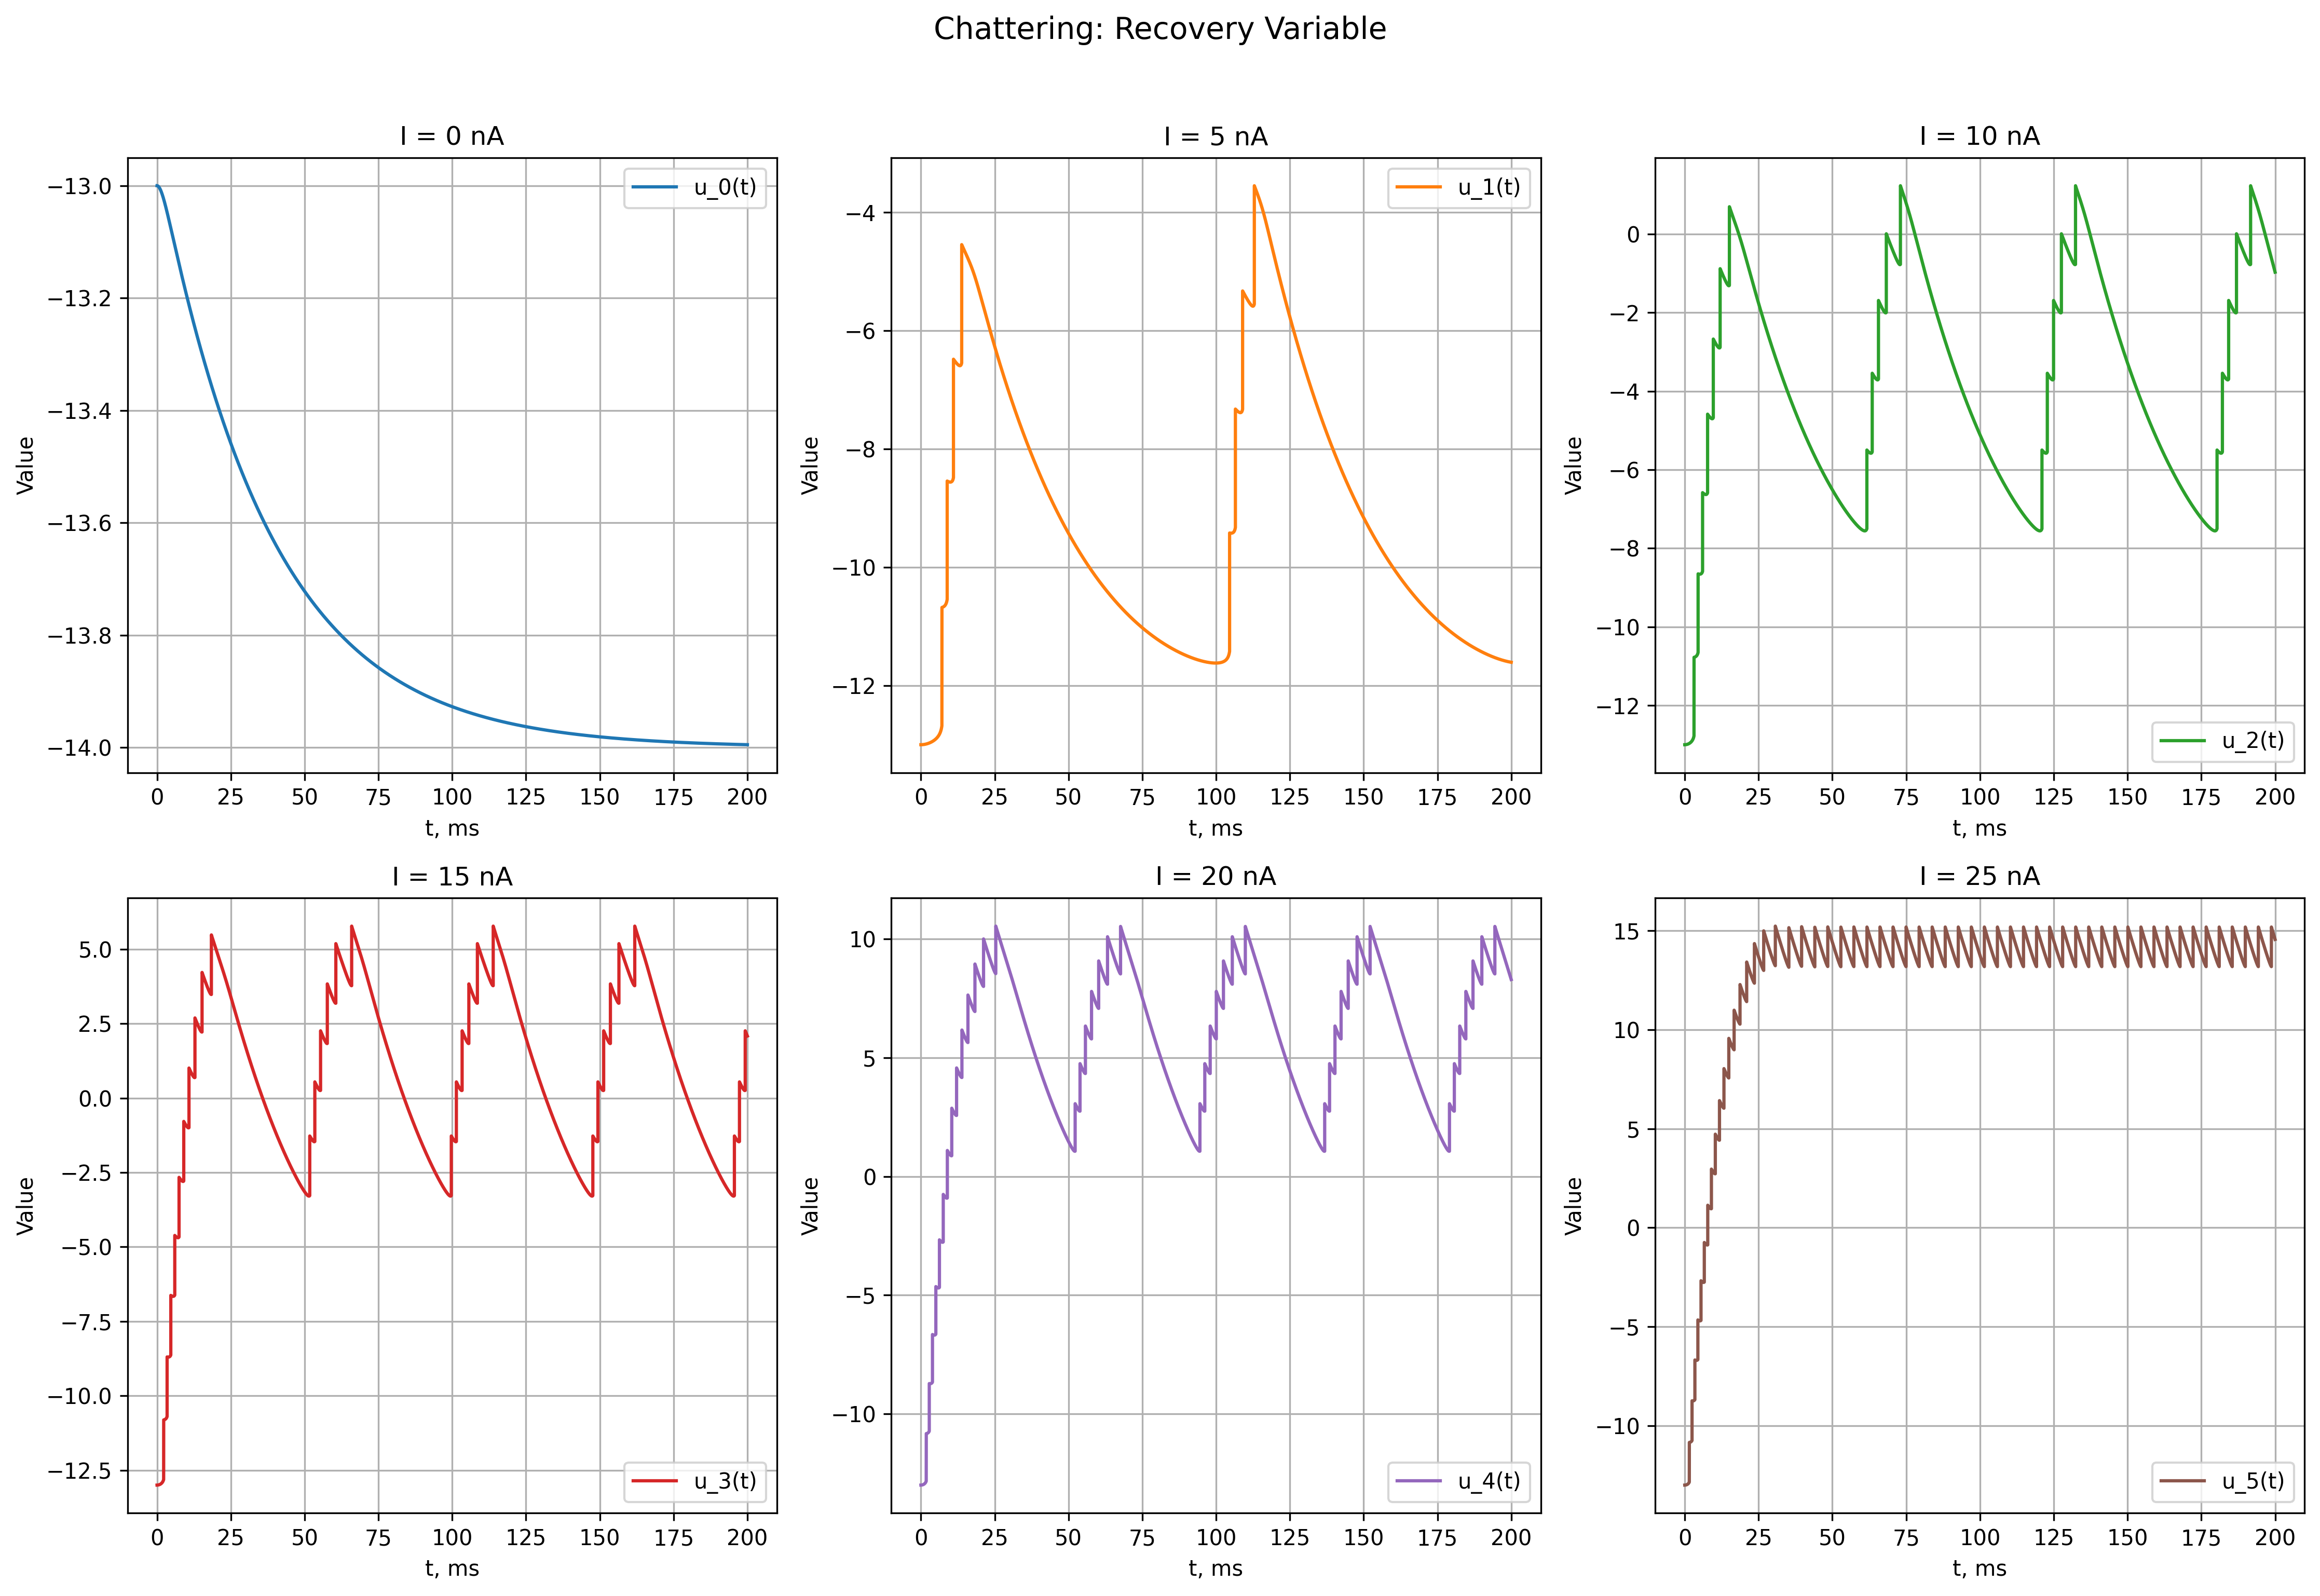
\includegraphics[width=1\linewidth]{pic/ch_different_I_recovery.png}}
	\caption{Визуализация $u(t)$ частотного нейрона для разных значений $I$.}
	\label{ch_different_I_recovery}
\end{figure}


\section{Анализ результатов}



\section{Листинг кода}

\inputminted[
breakanywhere=true, 
breaklines=true,
breaksymbolleft=\small\carriagereturn, 
frame=lines,
linenos,
fontsize=\footnotesize,
baselinestretch=0.8
]{python}{big_file.py}
\captiontextt{Листинг 1 --- Исходный код программы}





\endinput% Вторая глава
\chapter{Построение сети из двух связанных нейронов}
\label{ch:chap7}

Будем рассматривать гетерогенную сеть из двух нейронов: одного регулярно-спайкового(RS) и одного быстро-спайкового(FS). Введем переменную $\sigma$, характеризующую силу связи между нейронами сети. Запишем дифференциальные уравнения для моделирования динамики связанных нейронов

\begin{equation}
	\begin{cases}
			\frac{dv_1}{dt} = 0.04v_1^2+5v_1+140-u_1+I_1 + \sigma(v_2 - v_1),\\
			\frac{du_1}{dt} = a(bv_1-u_1),\\
			\frac{dv_2}{dt} = 0.04v_2^2+5v_2+140-u_2+I_2 + \sigma(v_1 - v_2),\\
			\frac{du_2}{dt} = a(bv_2-u_2),\\
	\end{cases}
\end{equation}

вспомогательный сброс

\begin{equation}
	\text{если } v_i \geq 30 \, \, mV , \text{ то } \begin{cases}
		v_i \leftarrow c_i\\
		u_i \leftarrow u_i+d_i,
	\end{cases}
\end{equation}

Под синхронизацией в данной задачей будем понимать согласованное во времени функционирование двух объектов (нейронов сети)\cite{sem}. Для того, чтобы оценить уровень синхронизации в зависимости от заданной силы связи $\sigma$ введем функцию $s(\sigma)$, значение которой вычисляется по формуле

\begin{equation}
	s(\sigma) = \frac{1}{n} \sum \limits_{t = t_1}^{t_n} (v_1(t) - v_2(t))^2
\end{equation}

\endinput
\chapter{Проведение моделирования при различных значениях силы связи}
\label{ch:chap8}

\section{Визуализация}

\begin{figure}[h]
	\center{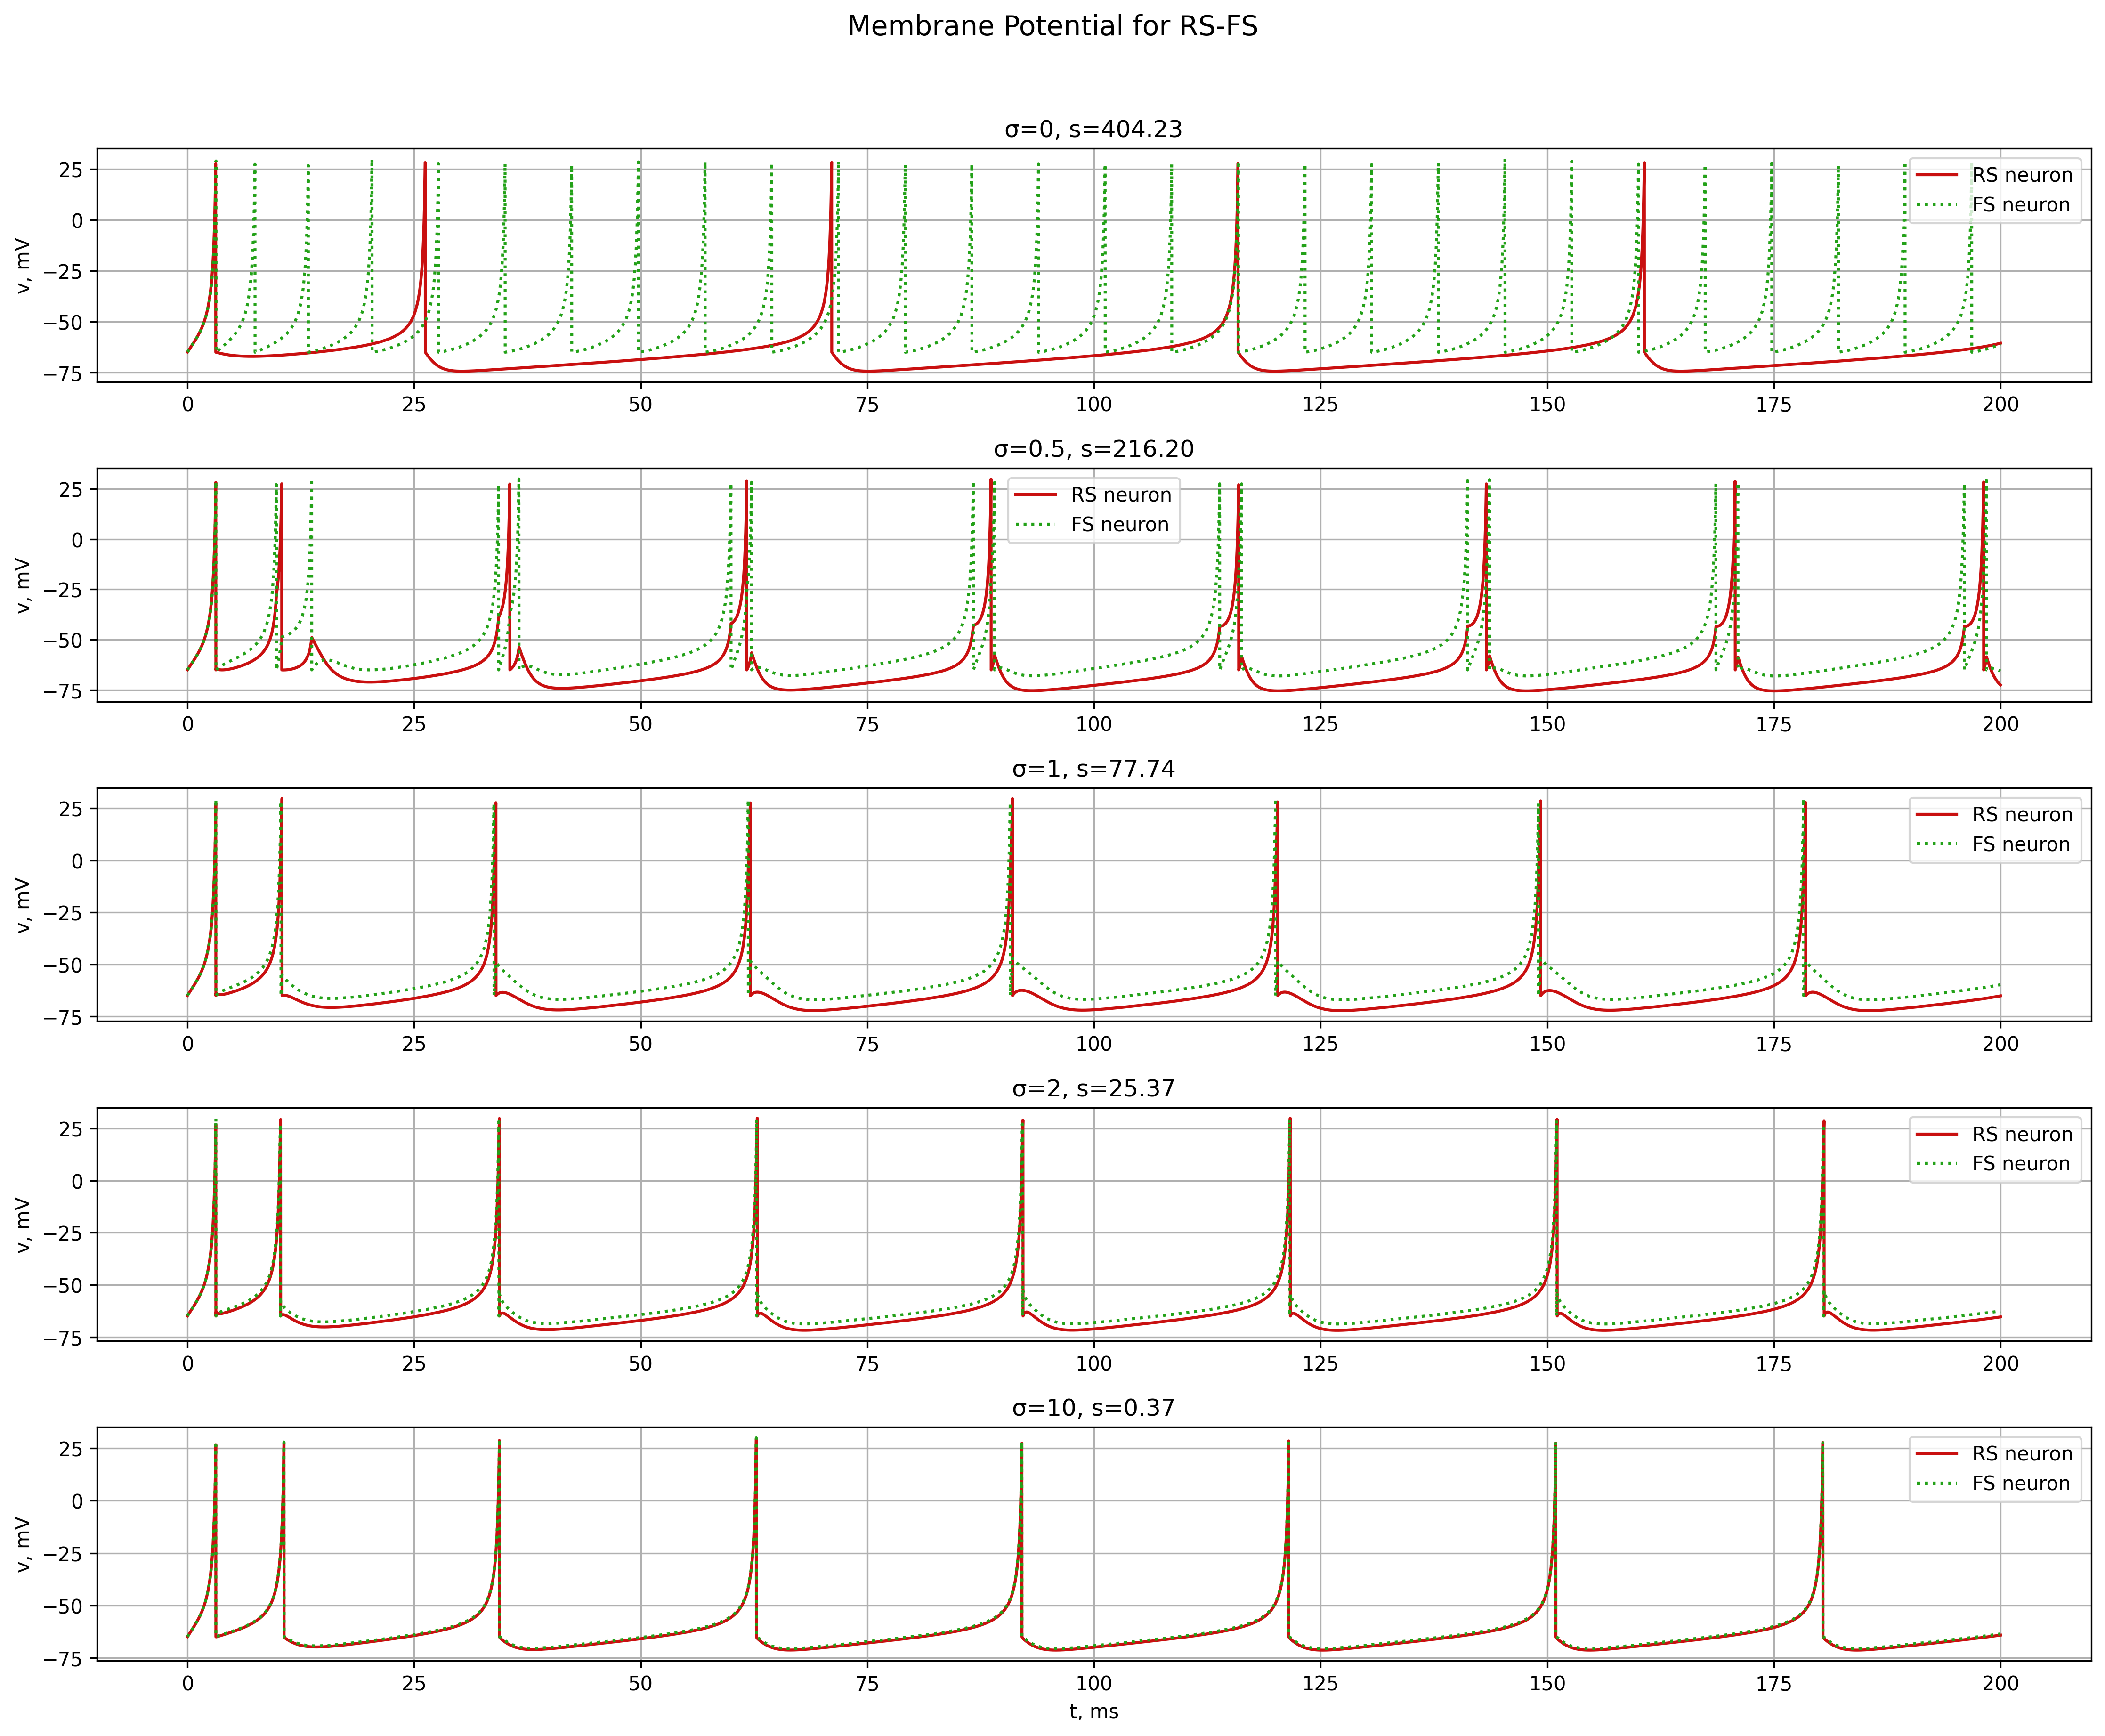
\includegraphics[width=1\linewidth]{pic/v_rsfs.png}}
	\caption{Графики мембранного потенциала $v_i(t)$ нейронов сети для различных значений силы связи.}
	\label{v_rsfs}
\end{figure}

\begin{figure}[h]
	\center{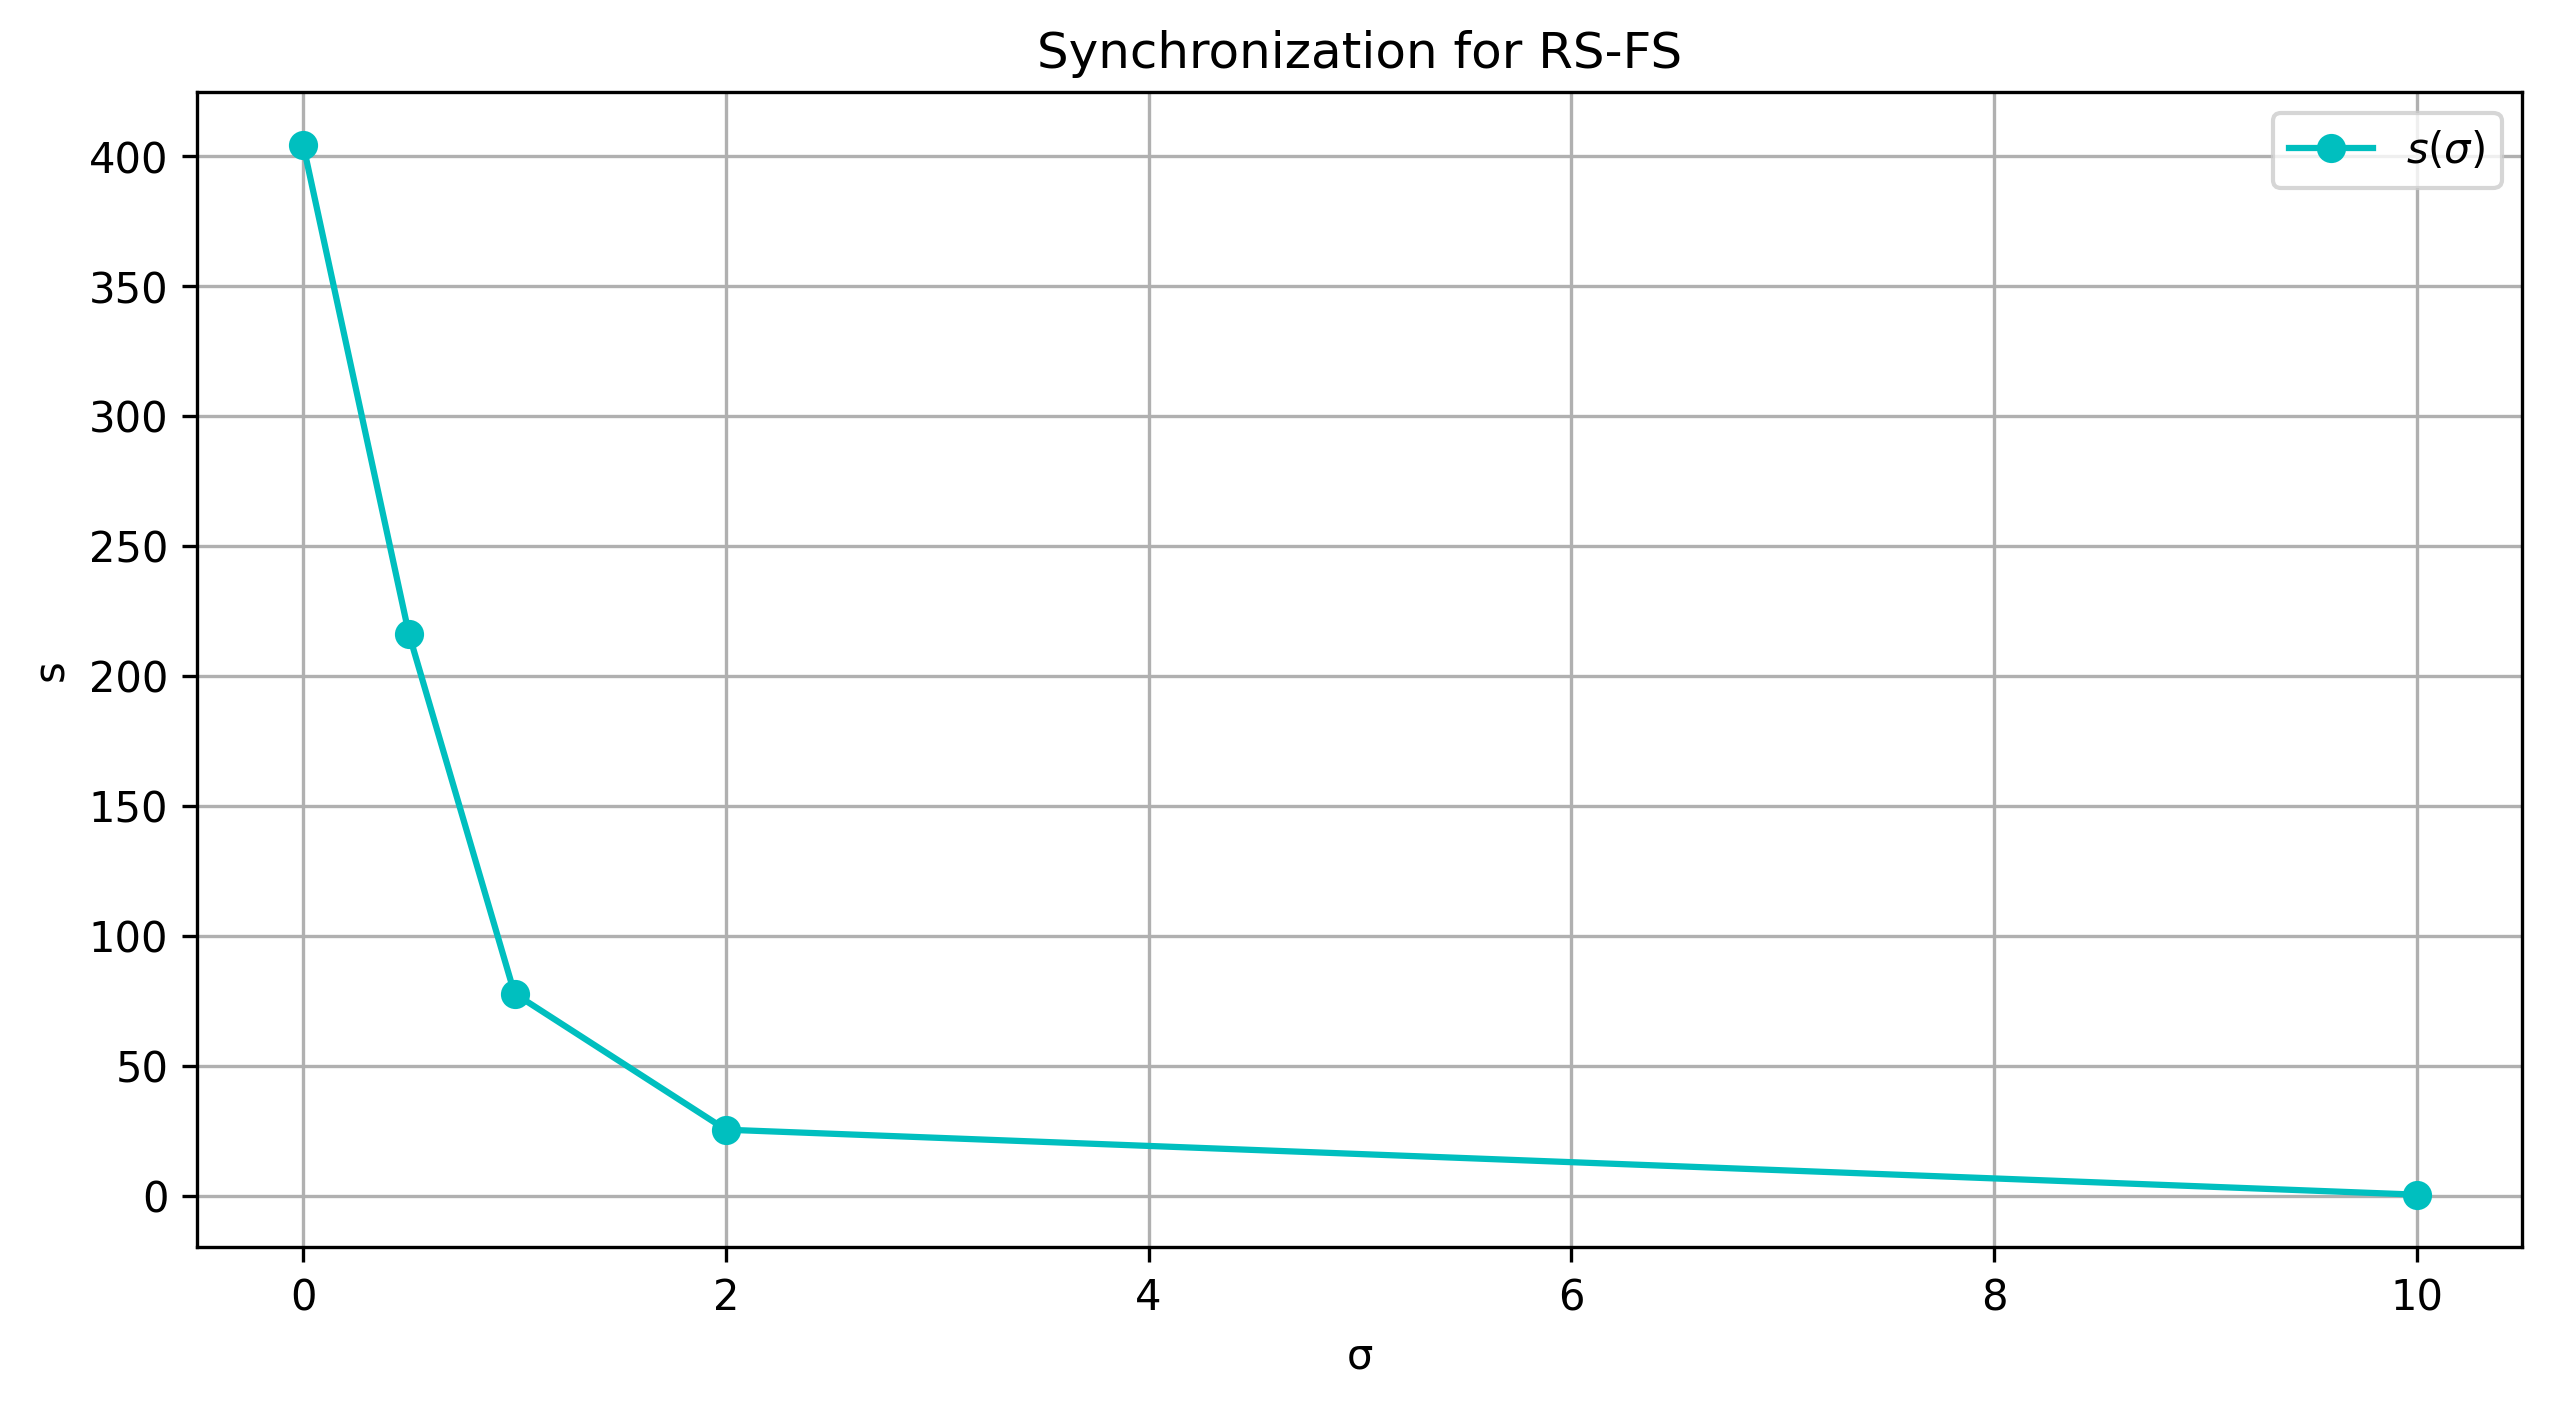
\includegraphics[width=1\linewidth]{pic/sync.png}}
	\caption{График синхронизации $s(\sigma)$ нейронов сети для различных значений силы связи.}
	\label{sync}
\end{figure}

\section{Анализ результатов}
Заметим, что при увеличении значения силы связи возрастает и уровень синхронизации нейронов сети (рисунок \ref{sync}). Кроме того, с увеличением силы связи динамика мембранных потенциалов обоих нейронов меняется, для RS-нейрона характерно повышение частоты спаек, для FS-нейрона -- падение частоты (рисунок \ref{v_rsfs}). В начале временного интервала заметно повышение частоты спаек с последующим увеличением временного интервала между спайками.


\section{Листинг кода}

\inputminted[
breakanywhere=true, 
breaklines=true,
breaksymbolleft=\small\carriagereturn, 
frame=lines,
linenos,
fontsize=\footnotesize,
baselinestretch=0.8
]{python}{big_file2.py}
\captiontextt{Листинг 2 --- Исходный код программы для моделирования динамики сети нейронов.}

\endinput
\chapter{Заключение}
\label{ch:chap6}
В ходе выполнения работы была изучена математическая модель нейрона Ижикевича. Рассмотрено влияние параметров модели на характеристики моделируемого нейрона. Выполнено численное моделирование изменения мембранного потенциала нейрона, а также вспомогательной переменной, отвечающей за восстановление мембранного потенциала. Теоретические данные были подтверждены проведенным моделированием, кроме того, было выяснено, что увеличение значения входного тока приводит к росту частоты спаек во всех рассмотренных наборах параметров модели.

 В последних главах работы была построена гетерогенная сеть из двух связанных нейронов. Выполнено моделирование динамики нейронов сети при различных значениях силы связи, совместно с определением уровня синхронизации нейронов сети. Было выяснено, что рост силы связи приводит к увеличению степени синхронизации динамики нейронов в сети.

\endinput

\printbibliography[title=Список использованных источников] % Автособираемый список литературы

\end{document}